\documentclass[a4paper,11pt]{report}

\usepackage{times}
%\usepackage[dvipdfmx]{graphicx}
\usepackage{amsmath}
\usepackage{amssymb}
\usepackage{amsfonts}
\usepackage[ruled,linesnumbered]{algorithm2e}
\usepackage{cite}
\usepackage{url}
\usepackage{listliketab}
\usepackage{lipsum}
\usepackage{calc}
\usepackage{multirow}
\usepackage{here}
\usepackage{amsthm} 
\usepackage{graphicx}
\usepackage{epstopdf}
\usepackage{lscape}
\usepackage{tikz}
\usepackage{esvect}
\usepackage{wrapfig}
\usepackage{tabularx}
\usepackage{rotating}
\mathchardef\mhyphen="2D
\usepackage{afterpage}
\usepackage{tabularray}
\usepackage{makecell}
\usepackage{booktabs}
\usepackage{multirow}
\usepackage{multicol}
\usepackage{csquotes}
\usepackage{listings}

\usepackage{lmodern}  % for bold teletype font
\usepackage{amsmath}  % for \hookrightarrow
\usepackage{xcolor}   % for \textcolor

\lstset{
  basicstyle=\ttfamily,
  columns=fullflexible,
  frame=single,
  breaklines=true,
  postbreak=\mbox{\textcolor{red}{$\hookrightarrow$}\space},
}

\newcommand{\tc}{T$_{c}$}

\ifpdf
  \DeclareGraphicsExtensions{.eps,.pdf,.png,.jpg}
\else
  \DeclareGraphicsExtensions{.eps}
\fi


\usepackage{enumitem}
\setlist[enumerate]{leftmargin=.5in}
\setlist[itemize]{leftmargin=.5in}


\usepackage[subrefformat=parens,labelformat=parens]{subfig}
%\usepackage{algorithm}
%\usepackage{algorithmic}
\usepackage{iitem}
%\renewcommand{\algorithmicrequire}{\textbf{Input:}}
%\renewcommand{\algorithmicensure}{\textbf{Output:}}
\usepackage{url}
\newtheorem{Definition}{\bf Definition}[section]
\newtheorem{Theorem}{\bf Theorem}[section]
\newtheorem{Lemma}{\bf Lemma}[section]
\newtheorem{Proof}{\bf Proof}[section]
\newcommand{\fig}[1]{{\gt fig.\ref{#1}}}
\newcommand{\eq}[1]{{\gt eq.\ref{#1}}}
\newcommand{\minmin}{\mathop{\rm min}\limits}
\newcommand{\bhline}[1]{\noalign{\hrule height #1}}  
\newcommand{\bvline}[1]{\vrule width #1}  

\usepackage{amsopn}
\DeclareMathOperator{\diag}{diag}

% \usepackage[top=20truemm,bottom=25truemm,left=25truemm,right=25truemm]{geometry}


\newtheorem{definition}{\textbf{Definition}}
\newtheorem{lemma}{\textbf{Lemma}}
\newtheorem{observation}{\textbf{Observation}}
\newtheorem{example}{\textbf{Example}}
\newtheorem{theorem}{\textbf{Theorem}}
\newtheorem{problem}{\textbf{Problem}}
% \newtheorem{proof}{\textbf{Proof}}
\newcommand{\argmax}{\mathop{\rm arg~max}\limits}
\newcommand{\argmin}{\mathop{\rm arg~min}\limits}

\setcounter{tocdepth}{3} %目次の深さ, toc: table of contents
\setcounter{page}{-1}

\setlength{\oddsidemargin}{9mm}
\setlength{\evensidemargin}{9mm}
\setlength{\topmargin}{5mm}
\setlength{\textwidth}{140mm}
\setlength{\textheight}{200mm}

\setlength{\parskip}{1em}
\setlength{\topsep}{0em}

\renewcommand{\baselinestretch}{1.0}

\newcommand{\vect}[1]{\mbox{\boldmath ${#1}$}}
\newcommand{\mat}[1]{\mbox{\bf {#1}}}
\newcommand{\unitvect}{\mbox{\bf 1}}

\newcommand{\eat}[1]{}

\newcommand{\authorlarge}{
  \vspace{35mm}\\
  {\LARGE March 2024}\\
  \vspace{10mm}\\
  {\Huge Luca Foppiano}
}
\newcommand\normx[1]{\left\Vert#1\right\Vert}
\makeatletter
\newcommand{\maketitleouter}{\newpage
\null
\vskip 5em 
\begin{center}
{\LARGE \@title \par} \vskip 1.5em {\large \lineskip .5em
\begin{tabular}[t]{c}\authorlarge
\end{tabular}\par}
\vskip 1em {\large \@date} 
\end{center}
\par
\vskip 1.5em
\thispagestyle{empty}
}
\makeatother

\title{\vspace{-15mm}{Automated Extraction and Curation of Materials Information from Scientific Literature}\vspace{65mm}}
\author{
  {\Large Graduate School of Science and Technology}\vspace{4mm}\\
  {\Large Degree Programs in Systems and Information Engineering}\vspace{4mm}\\
  {\LARGE University of Tsukuba}\vspace{10mm}\\
  {\LARGE March 2024}\\
  \vspace{10mm}\\
  {\Huge Luca Foppiano}
}
\date{}

\renewcommand{\baselinestretch}{1.}

% \usepackage[colorlinks = true, linkcolor = black, citecolor=black]{hyperref}
\usepackage[
    colorlinks=true,
    linkcolor=blue,
    filecolor=magenta,      
    urlcolor=cyan
    ]{hyperref}
\urlstyle{same}

\begin{document}

\maketitleouter
\maketitle

% \thispagestyle{empty} % no page number
% \include{01_cover}

\pagenumbering{roman} % page number : i, ii, iii, iv
\setcounter{page}{1}
%\newpage\thispagestyle{empty}\mbox{}\newpage


\phantomsection
\addcontentsline{toc}{chapter}{Abstract}
\begin{abstract}

The scientific literature, which contains vast human knowledge, is rapidly expanding, posing challenges in organising and retrieving information. 
Big data methods aid in uncovering patterns and making predictions and have long been applied in chemistry and biology, with other disciplines, such as Materials Science falling behind.
Materials Informatics (MI) is a discipline that leverages computational power to accelerate research in Materials Science by employing techniques like Density Functional Theory (DFT) computations and Machine Learning (ML) for material discovery. 
Despite advances, limited experimental datasets, such as SuperCon, hinder progress. 
SuperCon, a complex database for superconductor materials, faces challenges in consistent data collection. 
Automated processes are needed to extract data from new publications in a timely manner, and manual curation, which is prone to errors, requires careful tools and feature selection.

In this dissertation, we propose an end-to-end pipeline for extracting material information from the scientific literature to improve the efficiency and quality of material databases.
Our work aims to increase automated tasks to reduce the dependency on human intelligence to the minimum. 
The main contributions consist of developing ML-based models for recognising complex material expressions and other information from scientific text that is obtained directly from PDF documents. 
Material expressions are further processed with a parser that decomposes granular information such as name, formulas, doping, shape, etc. 
The extraction of properties is performed by combining with a general model for extracting physical quantities and measurements, called Grobid-quantities which support the identification and normalisation of units to the SI system. 
For evaluation and training, we developed SuperMat, a dataset of 142 superconductor articles. The dataset contains both entities and relations between them and was validated by domain experts.  
The automatic process collected a database with over 40000 extracted material-properties records from the related scientific articles from ArXiv. 
Finally, we proposed a curation interface to validate extracted data by combining an enhanced PDF viewer and a simple and sleek interface. Overall, the use of such an interface as compared with the traditional manual approach improved precision by 6\% and recall by 47\%. 
The models, dataset, and interface developed in this work will help increase the automation and accuracy of the processing of materials databases such as SuperCon from the scientific literature.

\end{abstract}
\newpage\thispagestyle{empty}\mbox{}\newpage

\phantomsection
\addcontentsline{toc}{chapter}{Acknowledgements}
\chapter*{Acknowledgements}
I express my deepest gratitude to all those who have contributed to the completion of this dissertation, as their support and encouragement have been invaluable throughout this academic journey.
First and foremost, I extend my sincere appreciation to my advisor, Professor Toshiyuki Amagasa, for his unwavering guidance, patience, and expertise. Their insightful feedback and constructive criticism have played a pivotal role in shaping the content and direction of this research.
I am grateful to the members of my dissertation committee for their time, expertise and valuable insights. Their diverse perspectives enriched the quality of this work and provided me with a broader understanding of the subject matter.

I would like to express my heartfelt gratitude to Dr. Masashi Ishii for his invaluable support and guidance during my time at NIMS (National Institute for Materials Science).
This research has greatly benefited from fruitful discussions and collaboration with Sae Dieb and Guillaume Lambard. 
I owe my ability to steer my career towards academic research in computer science and machine learning to the invaluable guidance, assistance, and support of Dr. Patrice Lopez. For more than a decade, Dr. Lopez has been a constant source of inspiration, providing me with the necessary tools and motivation to pursue my academic endeavours.
I express my gratitude to Dr. Laurent Romary for his assistance during my time at the National Institute for Research in Digital Science and Technology (INRIA), in Paris. Additionally, I am thankful to Dr. Mikiko Tanifuji for her support during my remarkable journey to Japan. 

I have been fortunate to have many individuals who have had a positive impact on my career, life, and accomplishments. Unfortunately, I am unable to mention each of them individually due to space constraints.

\pagebreak
\tableofcontents


\pagebreak
\phantomsection
\addcontentsline{toc}{chapter}{List of Figures}
\listoffigures

\pagebreak
\phantomsection
\addcontentsline{toc}{chapter}{List of Tables}
\listoftables

\pagebreak
\setcounter{page}{1}
\pagenumbering{arabic} % page number : 1,2,3

\chapter{Introduction}
\label{cha:introduction}
% Dependency between concepts
% -> materials science 
% -> Materials informatics 
% -> superconductivity 
% -> SuperCon
% -> Computational science 

% General introduction: 
% -> TDM 
% -> ML

% Materials science 
Materials science is a multidisciplinary field at the intersection of physics, chemistry, and engineering, dedicated to understanding, designing, and manipulating materials for a myriad of real applications. 
Central to this discipline is the exploration of the structure, properties, and performance of materials, ranging from metals and ceramics to polymers and composites. By delving into the microscopic and atomic scales, materials scientists seek to uncover the fundamental principles that govern a material's behaviour and tailor its properties to meet specific technological needs. 
This field plays a critical role in advancing technology and innovation, as discoveries in materials science often lead to the development of new materials with enhanced functionalities, improved performance, and novel applications across industries.

% Materials informatics 
Historically, breakthroughs in materials science often resulted from chance discoveries and unexpected observations, a process driven by serendipity and relying on trial and error. 
However, with the advent of advanced computational tools, machine learning, and big data analytics, materials informatics (MI) has emerged as a transformative methodology. 
Materials informatics is a multidisciplinary field that leverages computational methods, data science, and informatics techniques to accelerate the discovery and design of new materials, identify patterns, and predict material properties with unprecedented accuracy. 
Materials informatics not only expedites the discovery of novel materials but also enhances our understanding of complex relationships between structure, composition, and performance. 
This approach allows for a more efficient and systematic exploration of the vast material space, potentially leading to breakthroughs in fields such as electronics, energy, healthcare, and beyond. 

% Look at other fields 
In comparison of MI with well-established fields like computational chemistry and biology, we can discern not only the unique contributions of each discipline but also the collective progression towards harnessing computational power for transformative advancements in science and technology.
Computational chemistry is the earliest among the three, with its roots tracing back to the mid-20th century. The development of computational chemistry gained momentum with the advent of digital computers, and it has evolved significantly over the decades. Computational chemistry involves the application of theoretical methods and simulations to study the structure, properties, and behaviour of molecules, making it a well-established and mature field.
Computational biology, on the other hand, gained prominence later, particularly with the explosion of biological data in the post-genomic era. The field began to flourish in the late twentieth century and has since grown rapidly. Computational biology encompasses a broad range of techniques, including bioinformatics, molecular dynamics simulations, and systems biology, to model and analyse biological processes at various levels of complexity.
Materials informatics is a more recent entrant compared to computational chemistry and biology. Although the idea of using informatics approaches for material discovery has been around for some time, the field has gained significant traction over the past few decades, especially with the rise of advanced computing capabilities and the availability of large materials databases. 

Materials Informatics (MI) is founded on two key techniques: Density Functional Theory (DFT) computations and a data-driven approach using Machine Learning (ML). DFT computations, a core aspect of quantum mechanics simulations, delve into a material's electronic structure and properties at the atomic and molecular levels, providing a precise understanding that complements experimental data. On the other front, the data-driven approach utilises ML algorithms, from regression models to neural networks, for the analysis of extensive materials datasets. 
These algorithms decode patterns and correlations, enabling researchers to predict the properties of new materials or optimise existing ones. 
This combined approach, which integrates quantum-level insights with data-driven predictive modelling, accelerates the materials discovery process, facilitating the efficient exploration of diverse materials spaces.

Data-driven methods have significantly contributed to the design of new materials across various sub-domains, such as magneto-caloric, thermoelectrics, and superconductor materials. Despite the impactful role of these methods, a notable challenge lies in the limited availability of experimental datasets. 
Currently, the primary sources for such datasets in inorganic materials are Pauling File~\cite{Blokhin2018ThePF_paulingFile}, Starrydata~\cite{katsura2019data}, and SuperCon~\cite{ishii2023structuring}. 
The use of these databases highlights the need to broaden and diversify experimental data, improving the effectiveness and applicability of data-driven approaches in materials design. The addition of these datasets is crucial to advance the field, promote innovation, and expand the scope of materials discovery through data-driven methodologies.
SuperCon is the standard database for superconductor materials and it has been developed and manually maintained by NIMS since 1987. 
It consists of records of materials reported in scientific experiments and a large set of measured properties. 

A superconductor is a material that, when cooled below a critical temperature, exhibits zero electrical resistance and the expulsion of magnetic fields. This phenomenon, known as superconductivity, occurs in a variety of materials, with many of them requiring extremely low temperatures, often close to absolute zero, to manifest this unique behaviour. The critical temperature at which superconductivity emerges varies depending on the material. Superconductors have numerous applications, notably in the field of electrical engineering. They are utilised to create powerful electromagnets for applications such as magnetic resonance imaging (MRI) machines, particle accelerators, and magnetic levitation systems. Superconductors also play a crucial role in the development of high-speed, energy-efficient power transmission lines, since they can carry large currents without any loss. The potential for quantum computing and more efficient electronic devices is another area where superconductors are actively being explored, showcasing the interdisciplinary nature of their applications in physics, materials science, and technology.

SuperCon hosts about 32,000 materials records and a complex schema with about 200 properties, some of which have not been consistently collected~\cite{sommer20223dsc}. 
For example, the pressure applied to obtain superconductivity was reported in only 16 records; however, its studies and experiments date back to the 1970s, but it became more popular only at the beginning of the 21st century.  
However, SuperCon has been widely recognised for its quality and has been the data source for many attempts to design models that can predict Tc~\cite{stanev2017machine, le2020critical, Hamlin2019SuperconductivityNR}. 

However, using ML to predict Tc has some criticality that needs to be considered. 
The models have an intrinsic applicability domain, which means that predictions are limited to the patterns and trends encountered in the training set. 
This can lead to significant selection bias, making the models ineffective when applied to materials constituted by different compounds (or belonging to different classes). 
The variety of training data to be used should contain a relevant amount of non-superconductors materials to avoid training a model biased toward the assumption that a Tc always exists and render it ineffective when applied to new materials.
Now, the definition of non-superconductivity is tricky: if no superconducting critical temperature has been found, does not mean that one does not exist. It might be outside the range of current technological instruments. 
This leads to a conundrum when delving into the data: ignoring compounds with no reported Tc and maybe disregarding a potentially important part of the dataset for the sake of simplicity.
Simplifying too much could lead to an incomplete understanding of the factors that determine superconductivity and limit the ability to predict Tc accurately. 
Generally, in addition to these considerations, several SuperCon-related works attempted to integrate complementary data from other datasets. 
However, at the time of writing, only~\cite{sommer20223dsc} has aimed to directly enhance SuperCon.  
They successfully enhanced 9150 records with crystal structures from experimental results stored in the Inorganic Crystal Structure Database (ICSD). 
This recent work indicates that the SuperCon dataset continues to play a pivotal role in the landscape of superconductor research.

\section{Motivation}

The number of publications in superconductor research remained stable in the last 10 years\footnote{analysed on arXiv statistics on cond-mat category \url{https://info.arxiv.org/about/reports/submission_category_by_year.html}}.
It is reasonable to expect that future breakthroughs in superconductor research will be achieved through materials informatics, given its growing importance, and an updated SuperCon is to be considered a necessary condition. 

Two main challenges that SuperCon is facing motivate our work. 
The manual approach employed for compiling SuperCon is proving to be increasingly demanding in keeping up with the influx of new publications on time. The reliance on manual labour for dataset curation becomes a growing obstacle, as it demands specialised skills that are not readily available in the market. As the field of superconductor research evolves, the need for more efficient and scalable methods becomes apparent.
An automatic process is necessary to streamline and improve the population of SuperCon. 
The outline of the process comprises the ingestion of complete documents or text and the identification of materials and relative properties.  
In a small-scale preliminary assessment, we analysed the problem, identified several challenges to overcome, and proposed a data extraction framework~\cite{foppiano2019proposal}.

The expressions that identify materials are complex and lengthy, and their identification in the scientific literature poses several challenges.
Furthermore, the strict definition of what a material cannot be expressed in a synthetic sentence is valid for the whole discipline: There are differences between subdomains in materials science that make this process highly dependent on domain experts.

A material may be expressed in a multitude of partially overlapping definitions: as a single material, a single sample, a family, or a class.
Alternative approaches to naming exist, including the use of commercial names or sample designations, often arbitrarily chosen by researchers. Chemical formulas can be presented as stoichiometric expressions within these three categories, with possibilities such as ``Y-111'' or ``Ba(Fe1-xCox)2As2''. Examples of standard names include Oxygen or Magnesium Diboride, while some adopt abbreviated forms like Yttrium Barium Copper Oxide (YBCO). These varied strategies provide a range of options for nomenclature within the domains of chemistry and materials science, while the conventional method primarily involves the use of chemical formulas.

A class of materials refers to a broader category that shares certain fundamental characteristics or properties. Materials in the same class might be characterised by common structural features, electronic configurations, or other common characteristics that make them suitable for investigation. 
A family usually implies a more specific grouping that shares a closer genetic or compositional relationship. A set of materials with similar chemical compositions, crystal structures, or electronic configurations. 
A sample is just an arbitrary name chosen by the researchers that can overlap any of the previous definitions. 
To make matters more complicated, all these definitions are not strictly enforced and may fluctuate from one laboratory to another. 
In many papers, the authors talk about "high-Tc cuprates" referring to materials in the class of cuprates that also have high-Tc. This fallacious definition does not clearly describe which materials are included: \textit{"How high should Tc be to be considered 'high'?"}.

Manual curation remains a necessary component, but it does not guarantee complete elimination of errors. As reported by~\cite{sommer20223dsc}, their investigation identified more than 10,000 duplicate records within the SuperCon dataset at the time of their study, revealing instances where certain properties were inadequately populated. 
This underscores the inherent challenges and limitations associated with relying solely on manual efforts for data curation, emphasising the imperative to adopt more robust and automated strategies to enhance the accuracy and comprehensiveness of the SuperCon dataset.
The need for a curation-centric user interface and tools that allow the reduction of the manual bottleneck to a few minor actions, leaving to the automation of the tedious task of identifying main data in scientific publications.


\section{Problem definition}

NIMS encounters various difficulties in managing SuperCon. The task of updating the database to incorporate the latest research findings is becoming less feasible due to the scarcity of highly qualified individuals. Additionally, these individuals have to work on a task that offers minimal rewards.
The process of manual extraction may seem flexible, but in reality, it is not easy to control it in a cohesive manner, especially when it comes to incorporating the extraction of additional properties.

To expedite the extraction of information from scientific papers, it is necessary to develop an automated process. Working closely with domain experts is crucial as they can validate and provide guidance. Despite the potential challenges arising from different work methodologies, this collaboration enables the sharing of best practices across disciplines, leading to a comprehensive and unified solution.

\section{Contributions}
\label{sec-intro-contributions}
In the following section, we discuss the various contributions of this dissertation, highlighting their main relevancy. 
We created a novel flow compared to other works that ingest PDF documents directly. 
 PDF documents are the standard format for scientific publications, and the same ingestion interface works across all domains and publishers, allowing us to access the full text body (Section~\ref{sec:intro-pdf-contribution}). 
Furthermore, we extract a novel set of information (applied pressure and measurement methods) that, according to domain experts, is not fully understood and may contribute to achieving a breakthrough in superconductors research. 
Due to our choice to rely on ML for its resistance to noise and its ability to generalise well on unseen examples, we required high-quality training data (Section~\ref{sec:intro-material-related-extraction}). 
We constructed SuperMat (Section~\ref{sec:intro-supermat}), a novel dataset of 164 articles that contain annotations and relations between entities. SuperMat is a valuable addition to the field of MI as it helps address the limited availability of structured data sources.
In the realm of materials science, the information extracted is modelled as a triplet that contains material, properties, and conditions. Both properties and conditions can be expressed as measurements of physical quantities that are relatively uniform in most disciplines. 
However, while the conditions are constant between domains, the properties are highly domain dependent. As part of our contributions, we co-developed with Patrice Lopez a separate module related to Grobid based on ML to extract measurements of physical quantities (Section~\ref{sec:intro-ner-quantities}).
We then combined all of these techniques to perform a large-scale extraction from documents obtained by the ArXiv repository.
The automatically extracted database, SuperCon\textsuperscript{2} (Section~\ref{sec:intro-supercon2}) is the main contribution of our work. 
The database obtained addresses a critical requirement of NIMS to streamline the extraction of experimental data from scientific documents.  
Finally, as a last contribution to improve the quality and reduce the impact of manual curation, we developed a use interface that supports domain experts in data curation by providing means to quickly switch from the database record to the relevant context in the scientific documents and other functionalities that we demonstrate boost the quality of the curation output. 

\subsection{Extraction from the full-text body of PDF documents}
\label{sec:intro-pdf-contribution}
% PDF document extraction

Unlike other works~\cite{court2018auto, court2020magnetic, kononova2019text} that were predominantly based on web scraping or through the publisher API, we designed a novel data flow for the extraction of material-related information from PDF documents using an existing open source library, Grobid (Generation of bibliographic data)~\cite{GROBID}. 
While web scraping is rarely allowed (it breaks the usage agreement) or limited to public metadata information (e.g., abstract, authors, title), API access is often hindered by the necessity of agreements with publishers, making the gathered content difficult to share and challenging to replicate.
In both cases, each publisher carries its own limitations and data formats and must be treated separately; therefore, mining data directly from PDF documents enables us to emancipate ourselves from the type of data source.
Furthermore, the increasing abundance of open access literature~\cite{laakso2011the} provides means to access large-scale scientific literature (e.g., ArXiv (\url{www.arxiv.org}), ChemXiv (\url{https://chemrxiv.org/}), NIMS Material Data Repository (MDR)~\cite{tanifuji2019mdr} (\url{https://mdr.nims.go.jp})). 
We are then able to access all information from the scientific documents, including full text body, tables, and figures. In our work, we focus only on text, ignoring figures and tables to separate projects. 
Accessing the body differs us from other approaches~\cite{yamaguchi-etal-2020-sc} which are limited to abstracts that are short and synthetic. On the other hand, the body contains more information that includes experimental results in related works. 
However, it is acknowledged that abstracts, being synthetic and possessing a simpler structure, also play a role in data extraction.
This contribution is discussed in details in Chapter~\ref{cha:pdf_extraction}.

\subsection{ML-based extraction of materials-related expressions from text}
\label{sec:intro-material-related-extraction}

The scope of this work is to create databases of experimental data that are reported in the scientific literature. 
The structure to represent such information can be complex and strongly depend on each subdomain, which has its own characteristics and conventions. 
However, we can define basic information as consisting of three main information points: material expressions, properties, and conditions. 
Material expressions are a relatively loose concept that strongly depends on the domain of application. On the other hand, properties and conditions can be decomposed into expressions of measurements of physical units. 
This contribution is divided into three minor works that are discussed in Sections~\ref{sec:intro-ner-materials}, \ref{sec:intro-ner-quantities}, and \ref{sec:intro-supermat}.

\subsubsection{Identification of complex material sequences}
\label{sec:intro-ner-materials}
The field of materials science encompasses various disciplines, including chemistry, physics, and engineering. 
Material expressions within this field are typically lengthy and intricate sequences of characters. Materials themselves can be represented by chemical formulas, which may also include additional information such as the material's shape (e.g., crystal, single crystal, wire) and doping details (e.g., 2\% Zn-doped). It is common for scientists to define samples and assign arbitrary names to them. Chemical formulas often involve substitutions in either the amount of an element (e.g., La x Fe 1-x O 7) or the element itself (e.g., RE x Fe 1-x O 7 with RE = La, Cu) to represent multiple rare earth compounds. Frequently, samples are denoted by the amount of their doping variable (e.g., x = 0.1).

The identification and extraction of these entities is extremely challenging. 
We use machine learning (ML) techniques to implement the named entity recognition (NER) system. This approach offers several advantages, such as context awareness, robustness to noise, and better generalisation to unseen examples compared to rule-based methods. Additionally, we discuss the evaluation of three different architectures: Conditional Random Fields (CRF), Recurrent Neural Networks (RNN) based on Bidirectional chains of LSTM units, and BERT-based models.

The novelty of our approach can be summarised in four main components. 
First, the need for high-quality training data and the lack of resources in material informatics was raised to construct a new dataset called SuperMat (Section~\ref{sec:intro-supermat}) that contains annotated documents from superconductors research. This contribution is discussed in detail in Chapter~\ref{cha:supermat}.
Second, we wanted to reduce the risk that entities with low probability are overlooked. Our ML training strategy was designed to build models that are geared toward recall rather than precision (Section~\ref{subsec:ner-solution}).
Third, we train and evaluate three different architectures and select the best performing combination for each model. This flexibility is convenient, since each architecture has its own strengths and weaknesses.  
Finally, we had the need to extract a large number of entity types; therefore, we devised a two-layer approach where the second layer was specialised to segment only the material entities (Section~\ref{sec:intro-material-parser}).  
The original text is first processed and the main entities are extracted: materials and classes, properties (pressure, Tc), and conditions (measurement methods). 
Then, the material entities are further processed by a specialised material parser, where different modifiers such as doping, shape, substrate, chemical formula, and name are identified. 
Additionally, we incorporate the use of characteristics consisting of text patterns (such as uppercase and lowercase) and layout details (such as superscript, subscript, bold, and italic) that are exclusively extracted from the PDF structure.

\subsubsection{Construction of SuperMat: an annotated and linked dataset of superconductors research papers}
\label{sec:intro-supermat}
% SuperMat
A critical gap identified in existing resources is the absence of datasets consolidating relevant entities such as materials, conditions, properties, and their interrelations. 
Currently, no dataset offers a centralised solution for machine learning models, considering the intricate and inconsistent terminology prevalent in this domain. 
To rectify this deficiency, it is imperative to build a dataset, which forms the foundation for a methodology that involves iterative data collection and correction. This dissertation contributes to this endeavour by expanding the data set for superconductor materials. 
The inclusion of measurement methods, which enable the selection of experimental properties, and the incorporation of applied pressure, an underexplored area, holds the potential to pave the way for groundbreaking advancements.
This dataset has already been used for practical applications such as ML training~\cite{foppiano2023automatic}, Large Language Models (LLM) evaluation~\cite{foppiano2024mining}, and weighted clustering~\cite{dieb2022superconductor}. 
Chapter~\ref{cha:supermat} is solely focused on the creation of this dataset due to its extensive and intricate nature, which necessitated a detailed and comprehensive explanation.

\subsubsection{Parsing and normalising materials sequences}
\label{sec:intro-material-parser}

The need to standardise materials expressions arises from the fact that materials can contain a combination of different types of information, such as chemical formulas, doping, substrate, etc. For example, the expression La x Fe 1-x O 7 (x=0, 0.1) represents a formula with substitutions, where x can take values of 0 or 0.1. Another example is the expression La-doped Fe O7, which indicates the presence of doping. Furthermore, the amount of doping can be specified, as in the expression 2\% La-doped Fe O7. It should be noted that sometimes only the doping ratio is given, as in the case of x = 0.1. 
Related tools such as Text2chem~\cite{kononova2019text} and PyMatGen~\cite{Ong2013} have been used. 
However, these tools have limitations. They are limited to formulas, and because they are rule-based and have low tolerance to noise, they only work with "clean" input. 
For example, a non-stoichiometric formula like "La x Fe 1-x O 7 (x=0, 0.1)" would not be correctly parsed by these tools. 
To overcome this limitation, we integrated these tools after our second-level ML-based parser was developed to handle long complex sequences.
The "material parser" obtained is tolerant to noisy input and able to parse and convert material expressions to a structured form. 
This contribution is discussed in Chapter~\ref{cha:extraction-experimental-data}.


\subsection{Extraction of properties and conditions as measurements of physical quantities}
\label{sec:intro-ner-quantities}

Properties and conditions within the realm of science and engineering are often expressed through measurements of physical quantities. These measurements serve as a universal language, providing a standardised way of conveying information about various aspects of the physical world. Whether it is the length of an object, the temperature of a substance or the intensity of a force, these measurements encapsulate essential characteristics that form the basis for scientific understanding and technological advancements.
Measurement of physical quantities forms the backbone of scientific inquiry, fostering a collective language that transcends boundaries and enabling collaborative efforts in the pursuit of knowledge and innovation.
The use of different tools to identify materials and properties improves flexibility in handling and interpreting information, paving the way for broader support and integration of additional data in the future. Using specialised tools for material identification and property analysis, researchers and professionals can adapt to evolving research needs and technological advancements. This modular approach not only facilitates the incorporation of new measurement techniques, but also encourages interdisciplinary collaboration.
While measurements are, in appearance, consolidated information, their treatment is challenging: measurement units are often used differently in different disciplines, different systems (miles instead of metres, ATM instead of Pascal) of unit may be used because they are easier to understand for humans, but creating great confusion for machines (one of the most famous events in history was the Mars Climate Orbiter explosion). 
In this contribution, we present grobid-quantities, a Grobid module based on ML that specialises in the identification, extraction, and standardisation of physical quantities and measurement. At the time of development, grobid-quantities was the first ML-based open source project aiming to cover multiple disciplines (from biology to materials science) and systems of units (SI base, SI extended, imperial, etc.). 
This contribution is discussed in detail in Chapter~\ref{cha:measurements}.


\subsection{Large scale collection of experimental data from scientific literature: SuperCon\texorpdfstring{\textsuperscript{2}}{2} Database}
\label{sec:intro-supercon2}

The grobid-superconductors extraction tool represents a significant advance in data extraction efficiency and scalability, as demonstrated by the creation of the SuperCon\textsuperscript{2} database. 
This tool has proven to be remarkably efficient, achieving in a few days what would have taken years of manual effort. 
The original SuperCon database, which had been cultivated for two decades, contained approximately 33000 elements. 
With grobid-superconductors, the database has expanded to an impressive 40324 records, indicating a substantial increase in the amount of data processed. 
Given the high quality standard that SuperCon must meet, the SuperCon\textsuperscript{2} database serves as an important intermediate step in the automatic extraction process, bridging the gap between the original SuperCon database and the new data. 
The effectiveness of the tool is evident not only in its ability to match the scope of the original database but also in its ability to surpass it by capturing detailed information such as applied pressure and measurement methods. Once curated and validated, the data within SuperCon\textsuperscript{2} can seamlessly enhance the SuperCon database, leading to continuous improvements in the accessibility and depth of the stored scientific information.
This contribution is detailed in Chapter~\ref{cha:supercon2}.

\subsection{Techniques for mitigating the impact of manual curation}
\label{sec:intro-curation}

Validating automatically collected data poses significant challenges due to the potential inaccuracies and errors inherent in automated processes. 
To address this, we have designed a robust solution that features a staging area (SuperCon2) that is accessed through a curation workflow with a user-friendly interface. 
The interface offers functions to control the content of the database records, triggering the state transition to the underlying workflow. 
Requirements form domain experts demand that the underlying data be persisted, and the modification can be traced back to the original record. For this reason, our workflow generates a new record at each modification, maintaining a history which can be inspected at a later time. 
In addition, our system provides an enhanced visualisation of the original PDF document, allowing users to inspect and cross-reference the data efficiently. 
Furthermore, to continually improve the automated data collection process, our solution incorporates machine learning (ML) capabilities. 
Specifically, the system accumulates training data based on corrections made during the validation process, ensuring continuous refinement and optimisation of automated data collection through iterative ML training cycles.
In this work, we experimented and demonstrated that our workflow and interface can increase the recall of missing information from 45\% to 92\% and the F1 score from 52\% to 92\%. 
The experiments and the description of the curation interface are listed in Chapter~\ref{cha:curation}.

\chapter{Related work}
\label{cha:related_work}

This chapter is divided into different contributions and aspects of this research.
The chapter is organised from specific (text mining in materials science) to generic (NER, machine learning) works.

\section{Text and data mining in materials science}

\cite{court2018auto} propose a method to extract Curie and Néel temperatures from scientific papers. 
The authors initially considered using the original ChemDataExtractor for this task. 
Nevertheless, they observed that the rule-based approach resulted in reduced precision and recall due to the complexity of the scientific text. As a solution, they enhanced ChemDataExtractor by incorporating a semi-supervised relationship extraction algorithm.
This algorithm learns a typical pattern using a modified version of the snowball library. Typical patterns are stored and used to cluster new extracted patterns by distance similarity. 
The authors claim that they extracted 39822 records, consisting of 11340 Néel and 28482 Curie temperature records. 

\cite{court2020magnetic} propose another work where they process 74000 web-scraped scientific journal articles and build a database of 20,400 magnetic and superconducting phase transition temperature records and their associated chemical compound names.
The NLP pipeline operates in the following manner: text and tables from target journals were analysed to identify material formulas and temperatures. Subsequently, the identified entities were standardised, with temperatures converted to Kelvin, and doping issues resolved with specific rules.

% \cite{venugopal2021looking} proposes a framework to identify common trends in materials-science domains using keyword extraction from abstract and figure captions. Using a combination of LDA and NER, they constructed a topical map across the literature of glass-related research. 


SC-CoMIcs~\cite{yamaguchi-etal-2020-sc} describes a new corpus called SC-CoMIcs (SuperConductivity Corpus for Materials Informatics) tailored for the text mining of superconducting materials.
The corpus consists of 1,000 manually annotated abstracts related to superconductivity with seven named entity categories. Characterisation, process, property, material, element, doping, and value. The interannotator agreement scores were around 75-85\%, similar to other materials science corpora.
Experiments using SciBERT for the recognition of named entities achieved a 77\% F1 score, comparable to human agreement.
The learning curves indicate that the corpus size is mostly sufficient, although some categories could benefit from more data. The corpus was used to build a word search tool based on word vectors, demonstrating its utility for retrieving relevant terms by category. This paper shows the potential of text mining to extract key information from the superconductivity literature. The corpus provides a valuable resource to develop more capable natural language processing systems for material informatics.  

After our work, \cite{mitsui2023automatic}, published a work in which they describe a similar pipeline to extract superconductivity information from abstracts from the scientific literature.
It uses the SC-CoMIcs~\cite{yamaguchi-etal-2020-sc} corpus of 1000 annotated abstracts on superconductivity to train NER and RE models.
The author reports that they extracted material compositions, transition temperatures, doping information, and process details from 48,565 abstracts obtained querying the Elsevier Scopus API, for a total of more than 43,000 superconducting materials and 24,000 transition temperatures. 
Their work follows a similar approach to ours; first, they extract entities, and then they find the relations. 
However, their extraction density is limited by the abstract, which has only synthetic information. Taking into account their search query \textit{''‘supercond * AND tc OR transition temp''} they obtain around one superconductor material per abstract. 

There are several other works on TDM on experimental information from materials science; the most relevant are discussed in the following paragraphs. 

\cite{kononova2019text} describes a text mining system to extract and segment synthesis recipes from scientific articles. The articles are obtained through web scraping and the synthesis paragraphs are identified through classification. Subsequently, NER is implemented using RNN (specifically, BidLSTM + CRF) in the identified paragraph. This helps to identify the various components of the recipe, and the precursor, operation, and conditions of synthesis are extracted for a total of 19,488 solid-state synthesis reactions.
This work was limited to articles after 2000, due to the lack of available HTML/HTM version for older articles.

\cite{park2018text} proposes a text mining pipeline to extract metal-organic frameworks from scientific papers. In this paper, the authors focus on two main properties: surface area (SA) and pore volume (PV) mainly because they are the main properties related to the absorption properties of MOPs, are very commonly described in papers, and they have a very distinctive signature such as the units used to measure the quantity. 
The source data was obtained in HTML format and, after parsing, cleaning, and tokenising the text, the tokens were classified into 5 types using lexicons from the Cambridge structural databases. 
Moreover, they employ specific terms to recognise appropriate units that are used in unconventional ways. The resulting classified tokens were combined with each other (the material was connected to the corresponding attributes) using a rule-based algorithm.
On a sample dataset, the algorithm achieves 90\% and 88.8\% precision in extracting surface area and pore volume data, respectively.
When tested on a larger dataset of 2315 MOF papers, the precision drops to 73. 2\% for surface area and 85.1\% for pore volume. Errors occur due to complex sentence structures and incorrect identification of MOF names.

\cite{cruse2022text} introduces a nanoparticle-related dataset of 5,154 records extracted from 4.9 million materials science papers containing synthesis recipes and morphological information.
The authors successfully extracted 7,608 experimental and 12,519 characterisation paragraphs with compounds, amounts, synthesis actions, sizes, shapes, etc.
Limitations include the inability to distinguish targets from other morphologies and the lack of order information for seed-mediated syntheses.

\cite{ghosh2022band} develop an automated approach to extract band-gap values and relate them to chemical compounds in the titles and abstracts of articles.
The authors extended ChemDataExtractor with a new BandGapParser to identify band-gap information.
On a sample of 415 papers, the system achieved 51.32\% correct, 36.62\% partially, and 12.04\% incorrect extractions.
Errors are due to incorrect extraction of chemical entities, band-gap values, and to refer entities to values.
The approach was applied to 11,939 articles, extracting 10,608 band gap values for 10,292 compounds.
The limitation of this study is the evaluation that was performed by reviewing the extracted information rather than comparing it with the ground truth.

\cite{choudhary2023chemnlp} presents ChemNLP, a natural language processing (NLP) library and web application for analysing material chemistry text data.
It uses the publicly available arXiv dataset of ~1.8 million scholarly articles collected over 34 years.
The authors analyse publication trends, author names, taxonomy categories, and word frequencies in titles and abstracts.
An interactive web application was built to search for articles containing specific chemical elements and compounds.
As a demonstration, ChemNLP was applied to identify new superconducting materials by comparing the arXiv data set with a DFT-based superconductor database.
Machine learning techniques such as TF-IDF vectors, t-SNE clustering, and classification algorithms were used to categorise "cond-mat" arXiv articles with ~80\% accuracy.
ChemNLP provides an open dataset and tools to apply NLP techniques to the materials science literature for knowledge discovery.

\section{Machine Learning}

Machine learning (ML) has the ability to extract valuable implicit knowledge from data~\cite{keith2021combining}, which can provide fresh insights into existing problems.
The application of machine learning (ML) in intricate fields like chemistry requires the use of reliable and accurate data. 
However, it is important to note that the results obtained from ML models may not always be attributed solely to the domain knowledge incorporated, as there could be other concealed factors within the data itself~\cite{keith2021combining}.

Conditional Random Fields (CRF)~\cite{lafferty2001conditional} have been widely used in various ML tasks such as sequence labelling and NER~\cite{rodriguez2013sequence}. 
CRFs have been particularly effective in situations where multiple annotator-embedded label sequences are available, but there is no actual ground truth, as they provide a probabilistic approach to sequence labelling~\cite{rodriguez2013sequence}. 
Furthermore, CRFs have been compared with other machine learning models~\cite{tang2015aComparison} such as Support Vector Machines (SVMs)~\cite{boser1992training} and Structured Support Vector Machines (SSVMs) in tasks such as chemical entity recognition, demonstrating their versatility and effectiveness~\cite{tang2015aComparison, naseem2021aComparative, yang2019madex}.

% On the other hand, RNNs are known for their effectiveness in modeling sequential data and have been applied in various fields such as image processing, pattern recognition, and sound event detection (Kim & Kim, 2017; Graves et al., 2013).

The transition from CRFs to RNNs represents a shift from probabilistic graphical models to deep learning architectures. 
While CRFs are effective in capturing dependencies between input features and making predictions based on these dependencies, RNNs excel in capturing temporal dependencies in sequential data due to their recurrent nature. 
This transition is particularly relevant in tasks where the sequential nature of the data is crucial, such as speech recognition and acoustic event detection~\cite{graves2013speech,tian2020artificial}.
The use of recurrent neural networks (RNNs) has gained importance thanks to Long Short-Term Memory (LSTM)~\cite{sak2014long} and Gated Recurrent Units (GRU)~\cite{cho2001learning} for text processing tasks: classification and recognition. 
\cite{kim2022research, lyu2020combine,li2022channel, siswantining2023spratama} highlight the effectiveness of RNNs in processing sequential data, showcasing their superiority over traditional methods in natural language processing tasks.
Furthermore, the combination of RNNs, particularly bidirectional LSTM recurrent neural networks (BidLSTM), with CRFs has been explored for tasks such as word segmentation and morpheme segmentation, highlighting the adaptability of RNNs in sequence labelling~\cite{huang2015bidirectional}.

Particularly relevant is the work~\cite{lample2016neural} which proposes a new neural architecture for NER with an architecture based on a bidirectional set of LSTM chains. 
Bi-directional indicates that the text is computed from left to right (forward LSTM) and from right to left (backward LSTM). 
Such an architecture can incorporate information that is usually captured by hand-crafted features and/or gazetteers. 
Such architecture takes in input two types of word representation: character-based word representation, calculated from the supervised corpus, and unsupervised word representation, which is learnt from unsupervised corpora. 
The unsupervised word representations discussed were word2vec~\cite{mikolov2013efficient} but they can also be used for more recent ones: fastText~\cite{joulin2016fasttext}, GloVe~\cite{pennington2014glove}.

~\cite{peters2018deep} proposes a novel deep contextualised word representation that addresses two key aspects: a) capturing complex characteristics of word usage and b) incorporating the polysemy of words within linguistic contexts. The proposed approach calculates word representations based on the entire sequence. The network architecture consists of two bidirectional LSTM layers with dimensions 4096 x 512. These layers work in a complementary manner, with one predicting the next token from left to right based on the preceding tokens, and the other predicting from right to left. The study also highlights several important findings: a) instead of solely outputting the last layer, averaging the weights from all layers with a coefficient improves performance in downstream tasks, b) lower layers capture syntactic information while higher layers capture context-dependent aspects (semantic), and c) incorporating ELMo embeddings in both the input and output enhances tasks that utilise the attention layer after the RNN, but does not provide benefits for other task types.

The transition from LSTM-based RNN to transformers marks a significant change in natural language processing. The introduction of Bidirectional Encoder Representations from Transformers (BERT)~\cite{devlin2018bert} revolutionised language representation models by leveraging the power of transformers. Transformers, as proposed by~\cite{devlin2018bert}, replaced RNNs with self-attention, demonstrating the potential of this approach in language processing tasks~\cite{vaswani2017attention}. 
BERT, based on bidirectional transformers, offers a simple yet powerful architecture that allows efficient pre-training and fine-tuning with minimal task-specific modifications, leading to state-of-the-art performance across a wide range of language processing tasks such as question answering, language inference, and named entity recognition~\cite{devlin2018bert, joshi2019bert}. The bidirectional nature of BERT enables it to capture contextual information from both preceding and subsequent words, which is crucial to understanding the meaning of a word in a given sentence, thus outperforming traditional LSTM-based models~\cite{lee2019biobert, joshi2020deep}. Furthermore, BERT's ability to handle long-range dependencies and its superior performance in sequence labelling tasks, such as NER and RE, has been demonstrated in various studies~\cite{jung2021dg, hafiane2020experiments,kim2020korean}. Furthermore, the effectiveness of BERT in sentiment analysis, misinformation check and text classification tasks has been highlighted, showcasing its versatility and robustness in different NLP applications~\cite{ng2022modelling, shreyashree2022bert, taha2023automated}. 
However, it is important to note that while BERT has shown superiority in various language processing tasks, there are instances where CNN and LSTM models also perform competitively with BERT-based models~\cite{joshi2021evaluation,velankar2021hate}. 
In general, the advantages of BERT-based architectures lie in their conceptual simplicity, empirical power, contextual understanding, and superior performance in a diverse set of NLP tasks, making them a crucial advance in the field of natural language processing. 

In the following sections we first discuss all basic BERT-related work, and then the BERT-flavoured transformers related to materials science. 

\section{Transformers}

\cite{devlin2018bert} introduce BERT (Bidirectional Encoder Representation Transformer). 
While pre-trained language models have been discussed already in previous work~\cite{radford2018improving}, and can be exploited in two main ways: feature-based or fine-tuning. 
BERT aims to improve the fine-tuning approach and to solve the limitation of existing left-to-right language models, where each token can attend only to previous tokens in the self-attention layers~\cite{vaswani2017attention} of the Transformers architecture. 
BERT introduces an MLM (Masked Language Model) pretraining objective, where it randomly masks tokens in training examples and tries to predict them using the full context. This enables to use of both left and right contexts and pre-trains a fully Bidirectional Transformer.
Using the original transformer architecture~\cite{vaswani2017attention}, they define BERT\textsubscript{BASE} with L=12, H=768 and A=12 (110M parameters) and BERT\textsubscript{LARGE} as L=24, H=1024 and A=16 (340M parameters) with (L=layers, H=hidden layers, and A=attention heads).
The authors define the input as a sequence that can be a natural sentence, a paragraph, or a pair of sentences. They used a special separator [CLS] to start the sequence and convey the result of the final hidden state. For separating two sentences from a pair, they encode the separator with [SEP] and provide sentence embedding which states whether a token belongs to sentence A or B. 
Each token is encoded using position embeddings calculated using WordPiece using a dictionary of 30000 tokens vocabulary. 
The sum of the vocabulary token, the sentence token, and the position embeddings represent the input representation for each token. 
The authors defined two training objectives: Masked LM (MLM) and Next-Sentence Prediction (NSP). 
The MLM is prepared by substituting 15\% of the token's positions at random: 80\% of the time with [MASK], 10\% of the time with a random token, and 10\% of the time do not substitute. The reason is to provide the model with enough randomness so that the model does not always learn to replace the tokens with [MASK]. 
The NSP aims to identify whether a sentence follows another sentence. This is justified by the need to perform tasks such as answering questions in which relations between sentences are identified. 
BERT outperforms the present architectures on most NLP tasks and benchmarks such as GLUE, MNLI and SQUAD. 

After BERT was released, a multitude of flavoured models was released. We analyse the most important ones in the following paragraphs. 

\cite{liu2019roberta} reproduces the results obtained in BERT, revises the original architecture and proposes RoBERTa (Robust Optimised BERT Architecture), a revised BERT implementation that outperforms BERT on downstream tasks such as GLUE, RACE, and SQUAD benchmarks. 
The main modifications are summarised as follows. Instead of masking tokens statically only once during preprocessing when the data are duplicated 10 times, they apply different masking at each instance of the same example. Dynamic masking helps for less than 1 point percentage.
They suggest that changing the way the data is provided in the input, in addition to removing the NSP loss objective, improves the performance. 
In particular, providing full sentences from the same or different documents without NSP matches the original implementation of providing a pair of segments with NSP. 
Furthermore, results are even better by providing only sentences from the same documents and removing the NSP.
NSP removal was discussed in recent work~\cite{lample2019cross}.
Lastly, they propose training for a longer time, and supplying more data can improve the results: the original BERT was trained on 1M steps with a batch size of 250, while the RoBERTa was trained for fewer steps 31000 using a much larger batch size of 8000 examples. This setting requires a more scalable approach because the required GPU memory is larger. 
With these changes, RoBERTa is able to outperform BERT on most language understanding benchmarks such as SQUAD, GLUE, and RACE. 

\cite{Beltagy2019SciBERT} propose a scientific version of BERT, called SciBERT. 
SciBERT was trained on a random sample of 1.4M articles from Semantic Scholar (data set was not published): 18\% from computer science and 82\% from the biomedical domain. SciBERT was evaluated against BERT and outperformed BERT. 
Unlike BioBERT~\cite{lee2019biobert}, SciBERT was trained using a different tokeniser (SentencePiece instead of WordPiece). Most importantly, the tokeniser was re-trained from scratch using scientific text.
Another interesting aspect is that BioBERT was trained from a model initialised with the weight from BERT and overall was trained for a longer time and on more data. However, the limited coverage of the BERT tokeniser on scientific data penalised the performance on various downstream tasks.

\cite{yasunaga2020linkbert} introduces a new approach in pre-training a BERT model in two flavours: LinBERT and BioLinkBERT on the general text and biomedical text, respectively.
The authors introduce a novel approach which includes text from linked documents, and an additional objective function is to classify the type of link.
The pre-training data is aggregated as follows: a) Each example is structured as a pair of text sequences as in the original BERT. b) The pairs are aggregated by selecting the second segment (when available) as follows: randomly, from the same document, or from a related document. For the linkBERT, this only works for the Wikipedia corpus, exploiting the links between Wikipedia pages. For bioLinkBERT, the authors select sequences from related documents in the citation graph. 
The authors replace the NSP objective with the DRP (Document Relation Prediction), which aims to classify the type of relation between the two segments, giving three possible classes: contiguous, random, and linked.  
Evaluation metrics calculated on QA (extractive question answering), GLUE and SQUAD, outperform BERT. BioLinkBERT outperforms PubMedBERT~\cite{gu2020pubmedbert} on most NLP tasks. 

\cite{gu2020pubmedbert} pre-trained a biomedical-based model called PubMedBERT and evaluated using a newly assembled dataset called BLURB (Biomedical Language Understanding \& Reasoning Benchmark). 
The vocabulary was trained using a BPE (Byte-Pair Encoding) approach with a length of 30522, and trained on text from PubMed abstracts: 14 million abstracts, 3.2b words. 
The fact that they only use abstract could be a major limitation on the type of information that is used in the pre-training. 
They are the first to consider the concepts of "in-domain" (in their case, biomedical text) and "out-of-domain" (everything else). 
Their strong claim is that domain-specific pre-training from scratch can be superior to mixed-domain pre-training, which is in contrast with~\cite{hong2022ScholarBERT}. 
From the perspective of vocabulary, it is demonstrated by comparing scores from BioBERT~\cite{lee2019biobert} and SciBERT~\cite{Beltagy2019SciBERT} that vocabulary specificity improves performance in tasks applied to scientific text. 

\cite{su2022investigation} tested biomedical-trained BERT models on relation extraction in biomedical data. They demonstrate that downstream tasks on overlapping data that were used in pre-training bias the results for RE. In classification, they demonstrate that using only the information in the "CLS" token can be improved by adding complementary information from other layers. 

\cite{hong2022ScholarBERT} demonstrate that training with a multidisciplinary corpus gives better results than a transformer based on a domain-specific dataset. In addition, they also found that larger models do not always perform better. However, these results might be due to other issues they have introduced with their pre-training process. 
Previous work by~\cite{lample2019cross} has suggested a similar concept applied to translation tasks, where including cross-training information and, in particular, the addition of data in different languages not only boost the performance in translation but also help the performance in non-translation tasks. 


\section{Materials science BERT-based pre-trained transformers}

In this section, we analyse the BERT-based transformers that were pre-trained using materials science text. We provide a comparison evaluation of all of these transformers as a comparative measurement. 

\cite{pranav2023a} propose a material-property extraction for polymers, based on a fine-tuned BERT model on 2.4 million abstracts. They report that their NER system achieves higher results compared to other material-based pre-trained BERT models. Properties are connected to materials using a heuristic approach to find the closer entities.
With their system, they extract more than 300000 records of polymers and properties from the 2.4 million abstracts. 
However, the article does not provide information on data contamination between pre-training and evaluation: we do not know whether there is any overlap between the evaluation datasets, PolymerAbstract~\cite{huan2016a} and the training set of 768 abstracts. 
Moreover, it is not indicated whether their model can generalise properly, providing out-of-domain information of their evaluation dataset compared with the training set. 

\cite{huang2020batterybert} is another specialised set of specialised BERT models that focus on scientific articles related to batteries. In this work, the authors experiment with different approaches for fine-tuning, continuing a generic BERT training (batterybert), a SciBERT training (batteryscibert), or training from scratch a new model based only on text from battery research (batteryonlybert). The main differences are provided by the different vocabularies, where batterybert and batteryscibert are constrained by the original vocabulary, the batteryonlybert vocabulary was trained from scratch and could model more accurately the terminology used in the battery research articles. 
In document classification, batteryscibert obtained the highest score. SQuad evaluation (extractive Q\&A dataset) surprisingly showed better scores with batteryBERT. This work demonstrated the importance of having a solid base with general text as well as scientific information to provide a model that can generalise and adapt to multiple sets of situations where it could be used. 

\cite{guo2021automated} proposes a two-stage deep learning framework for extracting chemical formulas and applying a ''Role labelling`` in the description of the chemical reaction. 
Following a common schema Extract-Link, they first extract all references to chemical compounds and, subsequently, label each compound with its role in the reaction description. 
They introduce a chemical-focussing pre-trained BERT flavour followed by a task-adaptive encoder (ChemRxnBERT) that provides a role labelling method. 
The authors created a small dataset for fine-tuning chemical reaction annotations composed of relevant paragraphs containing chemical reactions extracted from articles in various chemistry journals. 
Role labelling was implemented in cascade by providing the main material between special tokens ([P], [\\P]) which are then linked to the other extracted entities. Since the sequence is shallow, it can link only one material with the rest of the reaction. Therefore, multiple passages are necessary if multiple products are present in the reaction paragraph.  


% \section{Experiments in fine-tuning Transformers}

% ~\cite{dominic2018revisiting} revisit the hyperparameters when training deep learning networks, focussing, in particular, on batch size and learning rate. The authors discuss a different approach for convolutional neural networks and report that a minibatch size of as low as m = 2, can provide better scores for medium-low datasets. However, for larger datasets, the batch size should not be greater than m = 32. 
% The batch size is an important hyperparameter, while it should be kept large for pretraining~\cite{liu2019roberta}, evidence indicates that higher performances will be obtained by smaller values for fine tuning. 

% \cite{smith2017dont} suggest a more performing approach could be to increase batch size instead of decreasing the learning rate while fine-tuning. 

% \cite{popel2018training} provides suggestions to improve the fine-tuning applied to translation tasks. Their finding can be summarised as follows: a) multi-GPU scaling is more effective than batch-size scaling on a single GPU, and moreover, it is better to run sequential processes on multi-GPU than parallel processes on a single GPU. b) Displaying the full learning curve is more effective than using the "early stop". c) comparing different datasets requires enough training time. Generally, large datasets converge in more time. 
% d) Big models should be preferred if training for several days. e) Sequence length should be kept as low as possible; depending on the dataset, this will allow a larger batch size. f) The batch size should be kept as high as possible (this was also confirmed by \cite{liu2019roberta}

% \cite{mehrafarin2022on} stress the importance of data size when fine-tuning and found that larger training affects mainly higher layers. In particular, the number of training steps is more relevant than the diversity of the dataset (??). 
% The authors compare a pre-trained BERT (baseline) with the corresponding fine-tuned models using 5 GLUE datasets of different sizes and other characteristics.
% To measure the amount of linguistic knowledge retained by the model, they designed a set of probes: bigram shift, object number, etc. They run the probes with frozen models and measure that up to layer 6 each subsequent layer retains more linguistic knowledge than the previous one. However, for fine-tuned models on large datasets, such information is lost as we move to higher layers. 

% \cite{hoffer2017train} suggests that the adjustment of the learning rate and the normalisation of the batch can reduce the generalisation gap (comparison between the training error and the validation error). Generalisation continues to improve for longer time even without any observable change in the training or validation errors. Large or small batches generalise the same if the number of iterations is adapted. 
% Finally, they claim that the change in the generalisation gap depends more on the number of updates than on the batch size. 

\section{Extraction of quantified properties and measurements} 
NER of physical measurement has a fundamental application in scientific texts and is relevant in other disciplines, including humanistic or social science. 

Attempts have been made to extract measurements from text using many approaches. At the time of this contribution, we identified the following related work. 

~\cite{aras2014applications} built a tool for the extraction of quantities based on Apache UIMA (Unstructured Information Management Architecture) in combination with pattern matching that circles a Finite-State Automata (FSA). 
The authors claim that UIMA and FSA are faster and better suited to process a large quantity of text.
Their work supports multiple constructs: values, intervals, and enumerations. Units are normalised to the International System of Standard (SI). 
Units are loaded from a configuration file that includes the normalised format. In the same work, they also combine keyword extraction and text segmentation, which are interesting challenges in the analysis of patent text. 
The authors used Quantalyze\footnote{\url{https://www.quantalyze.com/}}, a commercial tool designed to process patents, for comparison. They reported that Quantlyze had limited unit support. 

\cite{maiya2015mining} propose a search engine called MQSearch. Their work proposes a rule-based extractor for quantities and units that include the measured object. The extractor models each measurement using the five-tuple: (sign, number, error, scientific notation, units) where only numbers and units are mandatory. 
The data flow is comprised of four phases: preprocessing to mitigate noisy and incorrect character extraction. 
Then, to recognise units, they expanded an ontology of units from the OBO Foundry with additional information from external sources and defined one associated rule for each unit. The ontology is exploited to recognise the measured object. 
Quantities are extracted similarly with a set of regular expressions. 
The last phase is post-processing, which is used to discard possible wrong or invalid values. 
They also present a SoLR-based search engine that allows for a search using the extracted units, values, and measured objects. 

\cite{agatonovic2008large} built an extractor for patents using GATE (General Architecture for Text Engineering). 
Although GATE provides plugins for machine learning, they implemented their extraction using a lookup to a gazetteer and a database containing the transformation rules between one unit to another. 
The gazetteer was built from a set of units published by the GNU (Gnu's not Unix) Foundation and comprises a set of 30000 units. In addition, they also recognise references within the text and patent information (e.g. patent number, country code). 
They built the annotation rules using the JAPE language, which is structured as a matching rule and action to perform. 
%The authors evaluate their tool on two aspects: throughput and accuracy. They created a Gold Standard corpus of 51 documents, reporting the accuracy of 

Although most of the works are based on English, there are also some contributions that focus on specific languages: \cite{hetsevich2014processing} investigated issues applied to Russian-derived languages (Russian and Belarusian). 
The authors make a consistent analysis of the challenges of Russian-derived languages. 
They proposed a solution based on finite-state automation with 350 graphs running on top of the NooJ\footnote{\url{https://nooj.univ-fcomte.fr/}} linguistic processor. 
Grammar covers three of the six grammar constructs (genitive, accusative, and nominative). 
The evaluation was carried out on a mixed corpus of 100,000 words and resulted in an F1 score of 82\%. 

\cite{berrahou2013extract} combine the use of an Ontological and
Terminological Resource (OTR) with the use of ML.
The OTR is used as a reference and can be updated with new units that are not extracted correctly or completely. 
Their aim is to use a modified string matching function to extract measurements and units. Thus, the main problem they try to solve is to reduce the search space using string-matching functions. 
They proposed a two-step process. 
First, they use a classifier to determine whether a sentence contains a unit or not. The classifier is built on a bag of words where the words are counted using three methods. TF, TF/IDF and BM25. The model is then built with three different algorithms which are then compared: Naive Bayes~\cite{john2013estimating}, decision three (J48), support vector machines (SVM) and Discriminative Multinominal Naive Bayes (DMNB).
In the second step, they match potential candidates in the OTR and use the string function to select the item that is more likely to represent the extracted one. On the basis of the similarity, they defined two thresholds which they can consider as variants of an existing unit or a new unit or to enrich the OTR and improve future recognition.

\cite{kang_extracting_2013} describe another rule-based solution in which they outperform the respective ML-based system. 
Their goal is to extract targeted information from laboratory test results from diagnostic devices examined by the US Food and Drug Administration (FDA). 
The authors developed a symbolic information extraction (SIE) system for extracting four types of entity: analytes (substance considered), specimens (where the analyte is measured), units of measures of the analyte, and detection limits of the diagnostic device in the exam.
The SIE is based on a combination of rules and dictionaries. First, the candidates are extracted and then ranked so that the most plausible ones are selected from the set. The units of measures targeted in this work are only a subset of all units and are specific to this particular subdomain in biology. 
They evaluated their SIE against three probabilistic learning approaches: CRF, SVM, and HMM. SIE outperforms ML-based models, except for the unit of measures where the CRF obtained the best scores. 

More related to materials science \cite{dieb2015framework} proposes to integrate relevant units of measurement when composing a small data set (392 sentences) for the development of nanocrystal devices. 
The data set focusses on identifying several properties, including the property value and units that are common in the domain. 
This work also leverages ML using a set of CRF engines, focussing only on a few entity types applied in a cascade. 

~\cite{hundman2017measurement} describes an integrated measurement extraction that focusses on the scientific literature in earth science. 
They developed a novel method that extracts context-related information from measurements. Instead of developing their own measurement extraction tool, they evaluated three reuse options. Quantalyze showed low recall in both the extracted measurement and the measured object and had technical limitations in integration, such as a lack of REST API. ~\cite{agatonovic2008large}, discussed previously, was discarded due to the need to maintain the rules. 
Therefore, they chose our tool, Grobid-quantities which had the advantage of requiring only labelled data and providing acceptable results in terms of precision, recall, and f-score. 

% After the publication of our contribution~\cite{foppiano2019quantities}, other works have been published, often focussing on a limited scope or specific language. 

% \cite{petersen2021geoquantities} describes a system that aims to extract MAR (Mass Accumulation Rate) information on geographical locations in marine science PDF articles. Since these types of measurement are complex and only applied in their specific domain, it is not surprising that the original version of grobid quantities does not support them. However, due to the fact that grobid-quantities is open source and actively developed, they successfully trained a version of grobid-quantities with data that allow the support of MARs. 


% While \cite{ning2022ameta} focuses on the temporal aspect quantities extracted from news feeds. Not relevant, developed later on.

% \cite{epp2021stereo} describe a framework for extracting results from documents. They extract three main pieces of information: statistical results, condition information, and topics from scientific papers. Although their aim is to document the following of the American Psychological Association (APA) guidelines, there are small variations in many cases. 
% Their system exploits a flexible wrapper induction approach for the extraction of statistics and conditions, which is Grammar-based Condition Extraction (GBCE) by inferring a set of rules from a subset of papers and applying them to the rest of the dataset. The experimental topics are extracted using an adaptation of the unsupervised Attention-based Aspect Extraction (ABAE) approach. 
% The authors use the CORD-19 dataset, 500 documents (0. 25\%) are used to learn the rules with the GBCE and extract information with precision 99\% for APA-compliant documents and precision 95\% for non-APA-compliant documents. 
% The rule-based nature is strongly dictated by the uniform structure of the writing style and possibly to a limited amount of units and measurements that are expected to be extracted. 

\cite{hao2016} extracts numeric laboratory test expressions from clinical trial eligibility criteria texts. 
They encode information using the TimeML specification language TimeML. The system presented Valx extracts: a) numeric values and units using regular expressions, b) using a hybrid approach with a knowledge base, they extract variables referred to as quantities. They cover different text representations (e.g., BMI, body mass index, etc.). Valx supports the association of multiple values to the same variable, for example, "40 and 60 years" associate both values to "years". Their tool supports normalisation to convert conventional units to international units. 

\cite{roy2015reasoning} describe an approach to formalisation of quantities and measurements that aims at extracting information from free text and inferring complex reasoning that includes the entities being measured and their quantity. 
The authors introduce QVR (Quantity Value Representation) with three constituents: Value (which includes values and ranges), units (which characterise the value), and change (which indicates whether there is a modification in the value, e.g. increases). 
The extraction of quantities is performed using a Semi-CRF and a bank of classifiers. 
\cite{roy2015reasoning} uses four types of feature that are calculated for each token (and a window including the three previous and following tokens): a) classification using a lexicon to identify whether it appears as a number, unit, etc., b) determining whether it contains a digit, all digits, etc., c) POS (part of Speech). Units are extracted by assuming they are adjoined to the numeric values. 
This work reserves a detailed discussion on quantities entailment, given a quantity value, and a text it is a 3-way decision problem: a) entail: when the quantity-value is supported in the context, b) contradicts when the quantity-value is not supported by the context, instead, the Q-V is different, c) no relation. 
The Quantity entailment aims to clarify whether units are confirmed by the context and if the way they are described can be defined as equivalent (e.g. 2 couples, 4 people). The quantity entailment is relevant for scientific text comprehension, especially for the description of experimental results in a very concise way containing multiple relative comparisons within the same paragraph, which makes it hard to understand. 

The works of \cite{taha2021identifying} and \cite{ho2021qute} focused on tables.

\cite{ho2021qute} describe a comprehensive query system in which they leverage previously extracted quantities, units, and context to answer questions containing measurement conditions. 
Their data model is described as triples of the form (entity, quantity, context) where the context gives more information and proof to quantity and entity. 
The triplet is computed offline in several steps: first, the quantity is extracted based on \cite{roy2015reasoning}, which we have described previously. 
Entities and quantities are referenced using the Yago knowledge graph, and different columns are related to their previous work~\cite{ho2021extracting} and the extracted data is used to create an index with conceptualised quantities. 
This idea is particularly relevant to our grobid-quantity work because there are very few works at the moment that leverage the extracted property and quantities, and through an international system normalisation allows the search by values and interval with the normalisation helping to increase the recall on quantities not in normalised units. 

\cite{taha2021identifying} assumes that the table columns are already identified and focusses on covering unconventional unit names (e.g. LTS as Litres), considering that the columns should have the same normalised unit. The authors evaluate and compare their system (PUC) in terms of currencies, data storage, length, mass, and volumes. For example, Grobid-quantities do not support currencies well because they hardly appear in scientific papers. At the moment of writing, Grobid-quantities does not support extraction from tables; however, since there is a plan to improve the table recognition in the Grobid library, this future work could be implemented within the same framework. 



% \cite{stanev_machine_2017} used data from SuperCon in combination with ICSD and AFLOW. 
% Only a small subset of materials in SuperCon overlap with those in ICSD: about 800 with finite Tc and <600 are contained within AFLOW. 
% The AFLOW online repository contains calculated properties, but the DFT results have been extensively validated with observed properties. 
% The work uses this subset of materials to incorporate structural/chemical information and electronic properties from the AFLOW Online Repositories into their models. 
% They predicted about 2000 compounds as candidate superconductors, with the vast majority being cuprates or compounds containing copper and oxygen. 
% There were also some materials related to iron-based superconductors, as well as 35 members that were not obviously connected to any high-temperature superconducting families.


% \section{Named Entities Recognition}

% \section{Relation extraction}

% \cite{wu2019enriching} discuss R-BERT, an enhanced BERT architecture that incorporate relation information and combine them by concatenating before the activation function. 
% This problem is part of the Semeval 2010 task 8 challenge~\cite{hendrickx2019semeval}, and is limited to relation classification considering that a relation has already been identified.


\chapter{Extraction from the full-text body of PDF documents}
\label{cha:pdf_extraction}
\section{Introduction}

PDF is a widely accepted format for sharing and presenting documents, as it ensures that the layout and formatting of the document remain consistent across different devices and operating systems. This is particularly important in scientific publications, where complex figures, tables, and equations need to be accurately represented.
PDFs are often used to create documents intended for printing, and scientific journals traditionally required high-resolution print-ready files for publication. PDF documents are well-suited for this purpose, as they can embed fonts and high-quality images, ensuring that the final printed output is of high quality.
In addition, PDFs can be signed digitally, providing a level of security and authenticity for scientific publications. This is important to ensure the integrity and trustworthiness of research findings, particularly in fields where reproducibility and transparency are paramount.
Although isolating trends in the Internet jungle is challenging, PDF documents account for about 85\% of the Common Crawl dataset\footnote{\url{https://commoncrawl.github.io/cc-crawl-statistics/plots/mimetypes}} and interest has been growing\footnote{\url{https://trends.google.com/trends/explore?date=2000-01-01\%202024-01-19&q=PDF}}. 
However, it is important to note that, while PDF has been widely used in scientific publications, there are emerging trends and technologies that challenge its status as a "de facto" format. For example, the rise of open-access publishing has led to the adoption of HTML and XML formats for online articles, allowing greater interactivity, accessibility, and searchability of scientific content.
However, those formats are penalised by the lack of standardised approaches, leading to a jungle of flavours of the same original format (e.g., JATS is one of the most widely used).

\section{Proposed approach}

Given the important role of PDF documents in the dissemination of scientific knowledge, supporting them natively is a necessary step to build effective TDM processes. 
However, the Grobid library (Generation of Bibliographic Data)~\cite{GROBID} provides the ability to parse and structure text from PDF documents, such as scientific publications or patents.
Grobid implements a set of pre-trained sequence labelling models using Conditional Random Field (CRF)~\cite{lafferty2001conditional}, Recurrent Neural Networks~\cite{lample2016neural}, and transformer-based~\cite{devlin2018bert} architectures.
Grobid performed best in the citation extraction task~\cite{tkaczyk2018evaluation}. Lastly, Grobid has been successfully extended to support several domain-specific problems, for example, recognition of astronomical entities~\cite{grobid-astro}, segmentation of dictionaries~\cite{khemakhem2017automatic}, software mention~\cite{software-mentions}. 
Among the various open source tools available, it is still actively developed and is used in several large-scale research repositories, such as Mendeley~\cite{mendeley-extraction}, ResearchGate (\url{https://researchgate.com}), Scite.ai (\url{https://www.scite.ai}). 

The Grobid offers several advantages. 
a) Grobid does not require one to make multiple agreements with different publishers to obtain input data, which can be obtained by the growing proliferation of open access preprint services. 
b) PDF support in Grobid allows one to focus on the processing of a single format instead of dealing with several XML flavours. 
c) It is integrated with pdfalto (\url{https://github.com/kermitt2/pdfalto}), a specialised tool for converting PDF to XML, which mitigates extraction issues such as invalid character encoding, reconstruction of the correct reading order, and supports the resolution of embedded fonts and the support for multicolumn documents. 
d) Grobid internal data model \textit{LayoutTokens} access information in PDF documents at a low level for each token: style (italic, bold, superscript, and subscript), font (font type, font size), positions (coordinates (a list of pairs x,y), offset position). Those information that can be exploited as orthogonal features for ML models.  
d) By parsing PDF format natively, Grobid gives access to full text, figures, tables, and thus does not limit our work to public information such as abstracts.
e) It provides access to a set of high-quality, pre-trained machine learning models for structuring documents.

In this contribution, we present Grobid-superconductors, a novel application of the Grobid library as a text mining pipeline for scientific publications in materials science.
Our approach differs from other related works in several aspects. 
1) Instead of abstracts, we provide support for full-text~\cite{mitsui2023automatic}.
2) There is no requirement for us to reach an agreement with publishers~\cite{kononova2019text}.
3) We focus on processing a single format instead of dealing with several XML flavours~\cite{kononova2019text}
4) We avoid web scraping~\cite{court2020magnetic} and other processes that require addressing each website differently and requiring to update regularly to follow potential changes in the websites.
5) We use low-level layout details as attributes in our machine learning models that handle intricate representations of materials. For instance, the inclusion of superscripts or subscripts (which may not always be present in XML-formatted documents provided by publishers) can be intuitively advantageous in identifying chemical formulas.

\subsection{Publisher's agreement for source data}
Obtaining scientific articles through publisher APIs or web scraping can be inconvenient for several reasons. First, many publishers restrict access, demanding subscriptions or pay-per-view models, limiting accessibility for those without institutional access or financial means. Additionally, web scraping can breach the terms of service of a publisher, leading to legal and ethical complications.
Another challenge is inconsistency in the data structure. Publishers often have different formats, making it difficult to create a standardised data set. 
APIs, if available, may have varying endpoints, data formats, and authentication requirements, adding complexity to the retrieval process.
API limitations, such as the number of requests allowed within a specific timeframe, can slow down data retrieval, especially with a large volume of articles. The lack of standardisation in metadata and content formatting further complicates the extraction process.
Cost is another consideration, as accessing articles through APIs or subscriptions may involve expenses, while open-access resources often provide content freely, reducing financial barriers for researchers.
Open access resources, including institutional repositories and preprint servers, offer a wealth of scientific literature in a consistent PDF format that represents a convenient means to access and process articles from these sources due to their accessibility and lack of legal constraints.

\subsection{Abstract versus full-text}
The abstract of a scientific paper, a concise summary located at the beginning of the document, serves as a quick overview that summarises the objectives, methods, results, and conclusions of the research in 150 to 250 words. 
Researchers frequently employ abstracts to assess the relevance of a paper to their work and for streamlined database searches. 
In contrast, the full text of a scientific article delves into comprehensive details, spanning sections such as introduction, methodology, results, discussion, and conclusions. This exhaustive account is crucial for in-depth literature reviews, detailed analysis of methodology, data review, and evaluation of the validity of conclusions.
Taking into account the perspective of TDM, both abstracts and full-texts play distinct roles. Abstracts, due to their succinct nature, are suitable for large-scale automated analyses, offering rapid insights into trends, topics, or keywords across a multitude of papers. However, full texts are amenable to more in-depth TDM, allowing for detailed extraction of information and revealing nuanced relationships between concepts, methodologies, and findings. 
Although previous studies~\cite{yamaguchi-etal-2020-sc} have used abstracts, our research focusses on extracting complex information from scientific documents using the entire fulltext.


\section{TDM pipeline}
\label{subsubsec:document-structuring}

Grobid-superconductors is structured as a three-step process illustrated in Figure~\ref{fig:pipeline-overview}. The input is a PDF document which is converted to an internal model composed of text passages, tokens, and features. Those three elements are then used to perform Named Entities Recognition (NER), which are then linked by a Relation Extraction (RE) process. 
The output is a structured object serialised in JSON format.

\begin{figure}[htbp]
    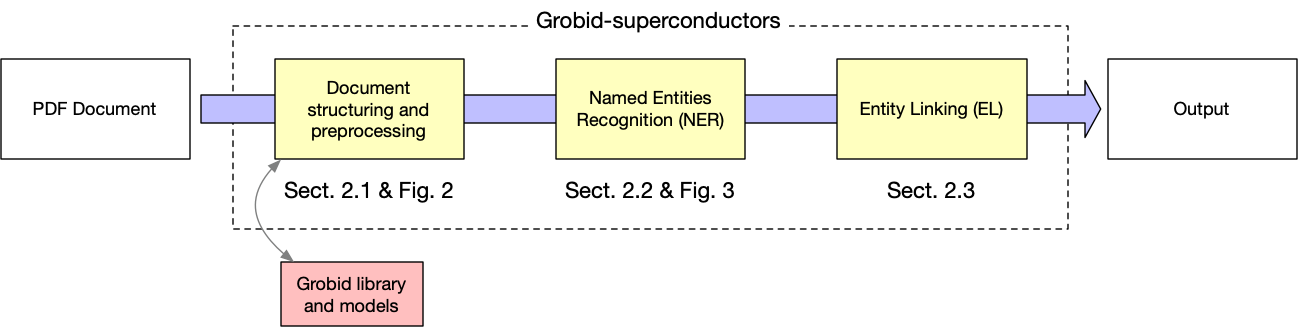
\includegraphics[width=\textwidth]{figures/automatic_extraction_supercon/schema-architecture-colors.png}
    \caption{Processing pipeline for extracting superconductors materials and properties. }
    \label{fig:pipeline-overview}
\end{figure}

\subsection{PDF document parsing}

The initial stage of our procedure involves using Grobid and Pdfalto to convert the PDF document. This results in the segmentation of raw data into a basic structure consisting of header, body, and annexes using the \emph{Segmentation ML model}.
These three structures are then parsed by a second Grobid model \emph{Fulltext ML model} that identify paragraphs, section heads, and references for body and annexes. 
We have created a custom process that analyses the structure and generates an internal model based on a list of text statements, tokens, and features. For example, the content of the tables is excluded, but the table captions are retained.
In the process, we can also assign textit{section} and \textit{subsection} information, as the results from the Grobid first level: header, body, and annex, and the second level (paragraph, table or figure caption, abstract, title) structures.

Header structures are parsed with the \emph{Header ML model} to identify bibliographic data. 
This aggregated version only includes information that is relevant to our TDM process. 
Our process selects a subset of bibliographic information from the header: title, authors, DOI, publisher, journal, and year of publication, and we consolidate them via Grobid to match the publisher's quality (even by processing the ``pre-print version'' of the publication).

\begin{figure}[htbp]
    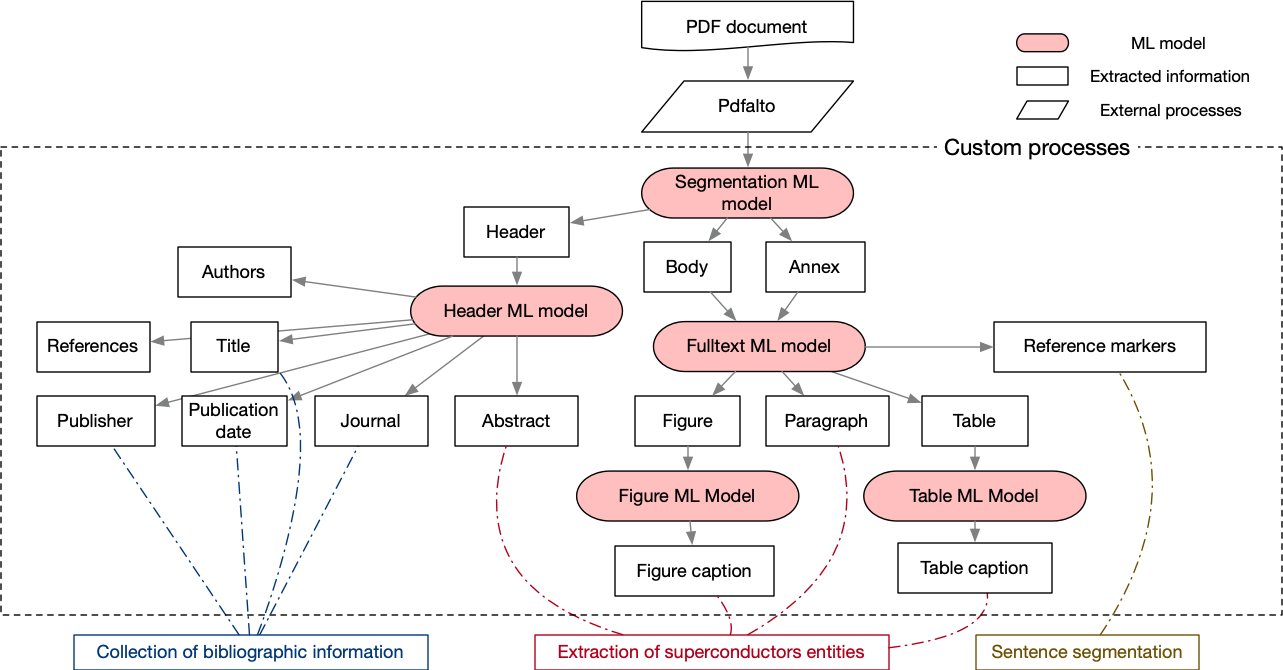
\includegraphics[width=\textwidth]{figures/automatic_extraction_supercon/document-structuring-colors}
    \caption{Grobid-superconductors extraction processes (bibliographic information, superconductor entity extraction and sentence segmentation) within the Grobid cascade data flow.}
    \label{fig:grobid-document-processing}
\end{figure}

\subsection{Sentence segmentation}
% Sentences vs Paragraphs 
An additional query concerning natural language processing (NLP) pertains to the choice between employing sentence-based or paragraph-based text.
While paragraphs can be extracted as part of the PDF document's layout, obtaining sentences requires an additional step of processing the text with a sentence segmenter. However, sentences are typically shorter, which offers advantages in deep learning.
In training and prediction, sentences will likely be shorter than the limit of sequence length that, which is for example, 512 tokens for transformers.
During training, sentences also use less memory and allow us to train models with a larger ``batch size'', which has been shown to improve efficiency and obtain better results~\cite{liu2019roberta}. 

\begin{table}[ht]
    \centering
    \caption{Results from cross-validation for sentence-based and paragraphs-based text. Measurements are micro average. P: Precision, R: Recall, and F1: F1-score.}
    
    \begin{tabular}{lccc}
        \toprule
        \textbf{Label}   & \textbf{P}   & \textbf{R}    & \textbf{F1} \\
        \midrule
        Paragraph-based  & 44.44        & 27.21         & 33.76       \\
        Sentence-based   & 48.41        & 50.00         & 51.70       \\
        \bottomrule
    \end{tabular}

    \label{tab:comparison-evaluation-sentences-paragraphs}
\end{table}

We chose to use sentence-based segmentation in Grobid-superconductors after performing small-scale preliminary experiments on our task. 
For the Named Entities Recognition (NER) task, we trained and evaluated a sequence labelling model for each approach (paragraph and sentence based) in four annotated documents (3/1 document partition for training/evaluation) from SuperMat, a dataset that we built~\cite{foppiano2021supermat} and is described in the following chapter.
As indicated in Table~\ref{tab:comparison-evaluation-sentences-paragraphs}, the F1 score increased by 17.94\% points when using sentence-based text.

For the RE task, we found in a previous study~\cite{foppiano2019proposal} that the sentence-based approach would favour higher precision, while the paragraph-based approach would result in greater recall.
% Therefore, we establish that a sentence-based approach is more beneficial than a paragraph-based approach for our tasks.

Since Grobid supports partitioning the documents up to the paragraphs, a sentence segmenter is necessary. The task has been long investigated, leading to the availability of many implementations. 
However, there are challenges in segmenting paragraphs from scientific text: reference reference markers (also called \textit{reference callouts}), formnulas, and other constructs may contain periods and mislead algorithms. 

Thanks to Grobid and the ability to recognise reference markers and formulas, we use the collected ones from the text as features to improve paragraph segmentation in sentences: segmentation is cancelled if the end of a sentence falls within the boundaries of one of these markers.
For example, a sentence such as "\textit{[...]The evaluation from (2021, Foppiano et al.) 
 offers a solid validation for our method}" containing a reference in the form ``Foppiano et al. and '' may be mistakenly segmented in the middle in the token ``et al.''. 

\section{Conclusions}

In conclusion, the application of innovative techniques, exemplified by Grobid, marks a significant milestone in the field of materials science. This effort represents a novelty for the first integration of such methods within the domain, showcasing the potential for transformative advancements. 
By sidestepping the complexities and expenses associated with signing agreements with scientific publishers and the intricate landscape of XML formats, this approach not only streamlines the dissemination process, but also liberates researchers from the often daunting challenges posed by conventional publishing models.

In the evolving landscape of scientific dissemination, where alternative means gain traction, it is noteworthy that the PDF format remains resilient as the "de facto" standard. The decision to publish through open access aligns with the current trend towards greater accessibility and openness in scholarly communication. 
The increasing availability of open-access articles further reinforces the utility and relevance of GRobid, positioning it favourably as a valuable tool in the arsenal of researchers seeking efficient and cost-effective methods for sharing scientific knowledge in the materials science domain.

This contribution was published as part of the paper "Automatic extraction of materials and properties from scientific literature"~\cite{foppiano2023automatic}.

\chapter{ML-based extraction of materials-related expressions from text}
\label{cha:extraction-experimental-data}
\label{subsubsec:extraction}
\section{Introduction}
This chapter discusses the Grobid-superconductors component responsible for data extraction through an intricate set of ML models encapsulated in data parsers for extracting material-related entities from scientific text. 
Identifying named entities in the field of materials science poses a formidable challenge, particularly due to the intricate nature of material expressions that are composed of complex and extensive sequences requiring meticulous attention. 
The definition of materials remains elusive in this domain, lacking a clear-cut delineation (refer to Chapter~\ref{cha:introduction}). Moreover, the boundaries within materials science are loose, subject to variations based on specific subdomains, and researchers focus on distinct aspects or phenomena associated with the materials.
Material expressions exhibit significant variability within superconductor research, incorporating various types of information within a single sequence. This can range from the chemical formula and doping ratio ("Zn-doped", "2\% Cu-doped", for instance) to the shape of the material (e.g., single crystal, wire, polycrystalline), as exemplified by expressions such as \texttt{single crystal La x Fe 1 x O 7 (with x = 0.1, and 0.2)}. Analysing non-stoichiometric formulas, in particular, presents a complex task, as these necessitate resolution with substitution values scattered throughout the paper.

The complexity inherent in deciphering such material expressions has propelled our exploration into the realm of Machine Learning (ML) as a means to model these intricate boundaries. ML has demonstrated its efficacy in various domains, including bioinformatics and chemistry~\cite{jiang2011astudy,tang2013recognizing,isazawa2022single}, often surpassing rule-based or lexicon-based approaches by achieving a delicate balance between flexibility and simplicity. 
However, it is essential to acknowledge that the success of ML is contingent upon the availability of data. This facet presents a notable challenge in material informatics compared to other domains. This challenge, in turn, has led us to create a novel dataset of annotated and linked text of scientific articles from superconductor research. In Chapter~\ref{cha:supermat}, we list the characteristics at the time of writing (number of articles, number of entities, etc.) and the methodology we used to construct it. 
Moreover, the notation incorporates supplementary text formatting choices, such as subscript and superscript, italic and bold. 
When these formatting options are converted to text, they are usually standardised to a regular font size, resulting in the omission of information.
To tackle this problem, Grobid has been crucial in preserving these data by utilising PDF layout information, as discussed in Chapter~\ref{cha:pdf_extraction}. This approach improves the accuracy and comprehensiveness of our identification of named entities in materials science.

We propose a novel solution that is organised as a two-stage process: initially, the text that is selected from various structures extracted by Grobid (Chapter~\ref{cha:pdf_extraction}) we pass them to a set of parsers that apply Named Entity Recognition (NER) and extract significant entities.
Next, the extracted entities are processed in pairs by a relation extraction (RE) process, and results are collected.


\section{Identification of complex materials sequences}
\label{subsec:ner-solution}

The process of identifying complex material sequences is a recently developed method that comprises four novel aspects.

\subsection{High-quality training data}
We have chosen to use machine learning for NER tasks due to the various advantages we have previously outlined. Machine learning techniques are particularly well-suited for extracting complex structures, although they require high-quality training data. We encountered a scarcity of such data, prompting us to create a new dataset. This project was an interdisciplinary collaboration between computer scientists and materials scientists. Domain experts specialising in superconductor materials provided guidance and technically validated the dataset. 
In Chapter~\ref{cha:supermat} of this manuscript, we provide a comprehensive description of the data model and a detailed account of the dataset construction process, which we refer to as SuperMat. The primary objective of Chapter~\ref{cha:supermat} is to shed light on the specific characteristics of the domain, including the types of data, providing examples and discussing their relationships.

\subsection{Positive sampling}
The SuperMat training data is prepared using a new strategy to improve the model's ability to identify entities with low probabilities, also known as "positive sampling". 
This approach prioritises recall over precision, aiming to capture as many entities as possible, even if it means sacrificing precision scores. 
Although some unrelated entities may be extracted, they are likely to be filtered out in the subsequent step of RE, which was developed as rule-based and thus more conservative. 
This decision is based on expecting the final result to undergo human validation. RE with a high recall may negatively impact efficiency, as the humans validating the data would need to spend significant time removing numerous incorrect records. On the contrary, extracting a few high-precision records will require less time to be ready for use.
From a holistic perspective, the recall-precision bias will be balanced between the two processes, as demonstrated in the end-to-end evaluation results, which will be further discussed in Section~\ref{sec:end2end}.
Positive sampling is applied by removing examples that do not contain any entities (negative examples, Figure~\ref{fig:training-holdout-set-distribution}a).
This approach provided an improvement of 2\% in both precision and recall compared to the result without sampling.
We tested additional sampling approaches, called active and random sampling, that target highly imbalanced datasets~\cite{lopez2021mining}. 
We tested them using ratios of negative examples of 0.1, 0.25, 0.5 and 1.0. However, they did not provide stable evidence suggesting any improvement, considering that our dataset was balanced. 

\subsection{ML architectures}
\label{sec:ml-architectures}
To determine the most effective architecture for our task, we assess several traditional machine learning (ML) methods supported by Grobid through Wapiti~\cite{lavergne2010practical} and the DL library DeLFT~\cite{delft}.
The architectures we consider include the linear CRF (CRF)~\cite{lafferty2001conditional}, Bidirectional LSTM with CRF (BidLSTM\_CRF)~\cite{lample2016neural}, Features Bidirectional LSTM with CRF (BidLSTM\_CRF\_FEATURES)~\cite{lample2016neural}, and a fine-tuned BERT-based transformer. For our specific task, we prefer to use the SciBERT~\cite{Beltagy2019SciBERT} encoder with a CRF as the activation layer (SciBERT). Unlike BERT, SciBERT has been trained on the scientific text and has demonstrated superior performance in various NLP tasks, including sequence labelling, classification, and question answering~\cite{Beltagy2019SciBERT}. It is worth noting that the CRF and BidLSTM\_CRF\_FEATURES architectures utilise features summarised in Table~\ref{tab:ML-model-features}.


\begin{sidewaystable}[ht]
    \centering
    \caption{Summary of the features used in the \textit{superconductors} and \textit{material} ML models. \textit{All} under Architecture indicate only BidLSTM\_CRF\_FEATURES and CRF.}
    \begin{tabular}{l m{30em} c c}
        \toprule
        \textbf{\#}   & \textbf{Feature}                                                                                                                                                                                                                                         & \textbf{Model}  & \textbf{Architecture} \\
        \midrule
        \textbf{1}    & current token                                                                                                                                                                                                                                            & all             & all                   \\
        \textbf{2}    & current token lower cased                                                                                                                                                                                                                                & all             & all                   \\
        \textbf{3-6}  & (four features) current token, prefix characters 1 to 4                                                                                                                                                                                                  & all             & CRF                   \\
        \textbf{7-10} & (four features) current token, suffix characters 1 to 4                                                                                                                                                                                                  & all             & CRF                   \\
        \textbf{11}   & information about capitalisation: first character (INITCAP), all characters (ALLCAPS), none (NOCAPS)                                                                                                                                                     & all             & all                   \\
        \textbf{12}   & digits content: all (ALLDIGIT), some digits (CONTAINDIGIT), no digits (NODIGIT)                                                                                                                                                                          & all             & all                   \\
        \textbf{13}   & (boolean) the token is composed of a single character                                                                                                                                                                                                    & all             & all                   \\
        \textbf{14}   & punctuation information and normalisation to placeholders: no punctuation (NOPUNCT), open or end brackets (OPENBRACKET, ENDBRACKET), various punctuation (DOT, COMMA, HYPHEN, QUOTE), open or close quotes (OPENQUOTE, ENDQUOTE), anything else (PUNCT) & all             & all                   \\
        \textbf{15}   & Shadow the numbers                                                                                                                                                                                                                                       & all             & CRF                   \\
        \textbf{16}   & Shadow any characters: ``x'' for lowercase, ``X'' for uppercase, ``d'' for digits                                                                                                                                                                        & all             & CRF                   \\
        \textbf{17}   & As the previous but compressed                                                                                                                                                                                                                           & all             & CRF                   \\
        \textbf{18}   & Font name                                                                                                                                                                                                                                                & superconductors & all                   \\
        \textbf{19}   & Font size                                                                                                                                                                                                                                                & superconductors & all                   \\
        \textbf{20}   & Font style: standard (BASELINE), superscript (SUPERSCRIPT) or subscript (SUBSCRIPT)   & superconductors & all                   \\
        \textbf{21}   & (boolean) if the token style is bold & superconductors & all                   \\
        \textbf{22}   & (boolean) if the token style is italic & superconductors & all                   \\
        \textbf{23}   & (boolean) the token is identified as a chemical compound by ChemDataExtractor\cite{chemdataextractor}                                                                                                                                                    & superconductors & all                   \\
        \bottomrule
    \end{tabular}
    \label{tab:ML-model-features}
\end{sidewaystable}

\subsection{Two-levels approach}
\label{sec:two-levels-approach}

To handle a diverse range of entity types, we must address the complexity of the information structures. 
Since most entities are structured around material names, we have implemented a two-level strategy to manage them effectively. 
In this approach, after processing the text with the first level ML models in the "Superconductor parser" (Section~\ref{Superconductor parser}), a dedicated ML-based "Material parser" for process the material entities (Section~\ref{material-parser}). 
While previous studies such as \cite{kononova2019text, court2020magnetic, dieb2015framework} have mainly focused on extracting formulas, we aim to extract a larger sequence and then deal with material segmentation separately. By adopting this approach, we can address the problems in separate instances, thus reducing their complexity. 
This parser can handle noisy data and be applied to various fields (Section~\ref{material-parser}).

\begin{figure}[htbp]
    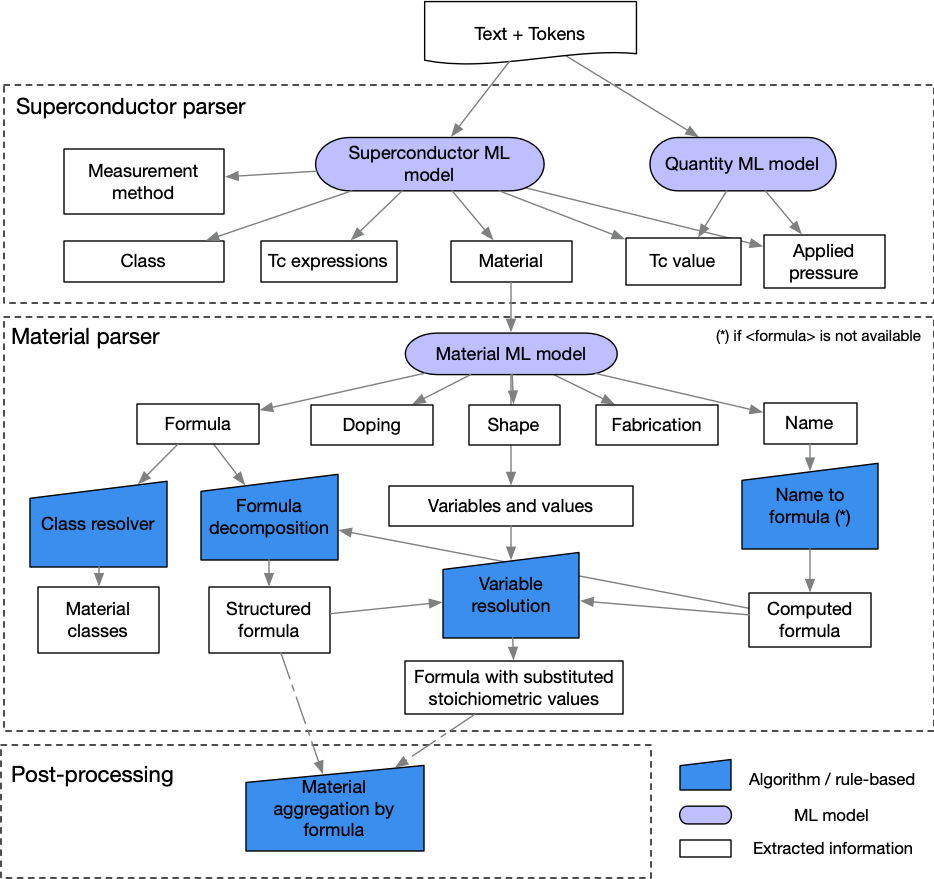
\includegraphics[width=\textwidth]{figures/automatic_extraction_supercon/schema-extraction-colors}
    \caption{\label{fig:extraction-ml-models-cascade-architecture} 2-level architecture for solving the NER task. The white rectangles indicate the extracted information (described in Tables~\ref{tab:superconductors-parser-entities} and~\ref{tab:material-parser-entities}).}
\end{figure}

The schema illustrated in Figure~\ref{fig:extraction-ml-models-cascade-architecture} comprises three main components: the ``Superconductor parser'', the ``Material parser'' and the ``Post-processing''. 

\subsubsection{Superconductor parser}
\label{Superconductor parser}
The ``superconductor parser'' extracts first-level entities (Table~\ref{tab:superconductors-parser-entities}) by aggregating the resulting entities from two ML models: ``Superconductors ML model'' and ``Quantities ML model''.
The ``Quantities ML model'' is reused from a separate Grobid module to extract measurements and physical quantities (Chapter ~\ref{cha:measurements}) and is limited in scope to target only entities of temperatures and pressures.
Overlapping entities of temperatures and pressures are merged, exact duplicates are removed, and the largest entities (in terms of string length) are preserved.
The ``Superconductors ML model'' was trained with SuperMat (Chapter~\ref{cha:supermat}), whose schema is summarised in Table~\ref{tab:superconductors-parser-entities}.

\begin{table}[ht]
    \centering\small
    \caption{Entities extracted by the superconductors parser.}
    \begin{tabular}{m{10em} m{20em}}
        \toprule
        \textbf{Entity} (\textbf{tag})              & \textbf{Description} \\
        \midrule
        Material (\texttt{<material>})              & Materials and samples names, formulas (including non-stochiometric formulas), substitution variables of values and elements, shape, doping, and substrate               \\
        Class (\texttt{<class>})                    & Groups of materials having similar characteristics or common strategic compounds that define their nature                                                      \\
        \tc~value (\texttt{<tcValue>})      & The value of the superconductor critical temperature                                                                                                          \\
        \tc~expressions (\texttt{<tc>})     & Expressions in the text that provides information about the phenomenon of superconductivity related to a value, interval or variation of \tc \\
        Measurement method (\texttt{<me\_method>}) & Technique used to measure or calculate the presence of superconductivity                                                                                     \\
        Applied pressure (\texttt{<pressure>})      & Applied pressure when superconductivity is recorded                                                                                                            \\
        \bottomrule
    \end{tabular}
    \label{tab:superconductors-parser-entities}
\end{table}

Entities of type \texttt{<material>}, which may contain heterogeneous mixed information, are passed to the ``Material parser'', which aggregates ML and rule-based methods.

\subsubsection{Material parser}
\label{material-parser}

The Material parser is an expression of different approaches. 
First, the entity is passed through a novel Material ML model to segment and identify its content (Table~\ref{tab:material-parser-entities}).
Then, different processes are applied depending on which information is available: 
\begin{itemize}
    \item Formulas are decomposed into a structured composition. We identify each element-stoichiometry pair (e.g., ``O'': 7.0) using text2chem~\cite{kononova2019text} and PyMatgen~\cite{Ong2013}; if only the material name is available, we lookup its formula (e.g., hydrogen to \textit{H}),
    \item Using heuristics, we classify the formula by assigning multiple classes as they are understood by superconductor researchers, for example, cuprate, oxides, alloys, etc.
    \item Using the variables and values extracted, we substitute them into partial formulas. For example, in \texttt{La 4 Fe 2 A 1-x O 7 (A=Mg,Co; x=0.1,0.2)}, we substitute \textit{A} and \textit{x} using their parsed values, and applying permutations, we obtain four \textit{resolved formulas}: \texttt{La 4 Fe 2 Mg 0.9 O 7}, \texttt{La 4 Fe 2 Mg 0.8 O 7}, \texttt{La 4 Fe 2 Co 0.9 O 7} and \texttt{La 4 Fe 2 Co 0.8 O 7}.
\end{itemize}

\begin{table}[ht]
    \centering\small
    \caption{Entities extracted by the material parser. }

    \begin{tabular}{m{10em} m{20em}}
        \toprule
        \textbf{Entity} (\textbf{tag})               & \textbf{Description}                                                                                                              \\
        \midrule
        Name (\texttt{<name>})                       & The canonical name of a material (e.g., hydrogen, PCCO, carbon)                                                                    \\
        Formula (\texttt{<formula>})                 & Chemical formula of the material (e.g., \texttt{Pr1.869Ce0.131CuO 4-}, \texttt{MgB2}, \texttt{La 2-x Sr x CuO 4})                  \\
        Doping (\texttt{<doping>})                   & Doping ratio and doping materials that are adjoined to the material name (e.g., \texttt{Zn-doped}, \texttt{2\% Zn-doped})          \\
        Shape (\texttt{<shape>})                     & shape of the material (e.g. single crystal, polycrystalline, thin film, powder, film)                                             \\
        Substitution variables (\texttt{<variable>}) & Variables that can be substituted in the formula.                                                                                 \\
        Substitution values (\texttt{<value>})       & Values expressed in the doping.                                                                                                   \\
        Substrate (\texttt{<substrate>})             & Substrates as defined in the material name                                                                                        \\
        Fabrication (\texttt{<fabrication>})         & Additional information that does not belong to any of the previous tags  (e.g., intercalated, electron-doped) \\
        \bottomrule
    \end{tabular}
    
    \label{tab:material-parser-entities}
\end{table}


\subsection{Post-processing}
Finally, after all entities are extracted, the post-processing aggregates different mentions of the same materials using the parsed formulas at the document-level.
For example, formula with partial substitutions such as \texttt{La 2 Fe 1-x O 7 (x = 0.1, 0.2)} will be aggregated with materials like \texttt{La 2 Fe 0.9 O 7} appearing in other sections of the same document.


\subsection{Extraction of relation from materials-related entities}
\label{subsec:re-solution}
\label{subsubsec:linking}

Relation extraction (RE) links materials and their corresponding properties. 
We explored different approaches, such as the use of dependency parsing~\cite{yoshikawa:2017acl, Tiktinsky2020pyBARTES, swayamdipta:17, zhou-zhao-2019-head} or machine learning~\cite{lin2016neural,hariharan2019relation}. 
Unfortunately, these methods were developed or trained using text from news articles, and their performances on scientific text were unsatisfactory. 
Another aspect is that our dataset was too small, in terms of the number of relations, to train any of these ML methods successfully. 
In particular, working with dependency parsers was extremely difficult due to their inability to districate in such complex writing. 
Compensating such poor performances resulted in the need to write over-complicated rules. 

We developed a rule-based algorithm that links together pairs of entities:
\begin{itemize}
    \item \textbf{material-tcValue}: The link between a material and its corresponding \tc.
    \item \textbf{tcValue-pressure}: The link between \tc~and its related critical pressure.
    \item \textbf{me\_method-tcValue}: The link between \tc~and its corresponding measurement method.
\end{itemize}

Entities of type \texttt{<tcValue>} are pre-processed through a classifier that establishes whether or not the temperatures refer to the superconductivity. This excludes temperatures referring to irrelevant properties (e.g., annealing, transition, Curie) that might be incorrectly extracted upstream.
This rule-based classifier combines the extracted entities of \tc~expressions (label \texttt{<tc>}) with a set of predefined standard terms.
If a temperature is not considered a \tc, it is excluded from the list of possible linking candidates.

Two scenarios are considered. First, if entities to be linked in the sentence are only two, they are linked automatically, else further rules are applied. 
If the word ``respectively'' appears in the sentence, we apply ``order-linking''. 
For example, consider the following sentence:
\begin{displayquote}
    P-or Ba-122  and Co-doped Ba-122 have lower \tc's of about 30 K and 24 K, respectively, which makes helium-free operation questionable.
\end{displayquote}
It contains the word ``respectively'', and by applying ``order-linking'', \textit{P-or Ba122} is assigned to \textit{30 K} and \textit{Co-doped Ba-122} to \textit{24 K}.


Suppose the word ``respectively'' does not appear in the sentence. In that case, we apply ``distance linking'' by defining the distance measurement \textit{d} as a value calculated as the number of characters between the centroid of each entity, measured in the number of characters.
Entities surrounded by parentheses are expanded to cover the "whole parentheses", and their centroid is updated.
As an example, in the sentence
\begin{displayquote}
    We tested two materials, MgB2 (Tc = 39 K) and FeSe (Tc = 16 K).
\end{displayquote}

\texttt{39 K} is closer to \texttt{FeSe} (\textit{d}=10) than to \texttt{MgB2} (\textit{d}=11). 
In this example, however, both temperature entities would be expanded to their containing parenthesis (e.g. ``\texttt{39 K}'' to ``\texttt{(Tc = 39 K)}''. 
In this case, the centre of the entity ``\texttt{39 K}'' is shifted to the left, from the initial value of 38 to 35, and the distance from \texttt{MgB2} is reduced from \textit{d}=11 to \textit{d}=8.
As a result, the \texttt{MgB2} entity is correctly linked to ``\texttt{39 K}''.

Distance calculation is also adjusted with the addition of ``penalties'' by doubling the calculated distance when specific keywords or punctuations (``,'', ``.'', ``;'', ``and'', ``but', ``while', ``whereas', ``which'', ``although'') appear between two entities because they represent a logical separation of predicates ~\cite{oka2021table}.
In the above example, the distance between \texttt{39 K} and \texttt{FeSe} would be doubled (\textit{d}=20), and the link would not be made.

\section{Results}

\subsection{Identification of materials-related entities from text}
\subsubsection{Experimental settings}

We used SuperMat (Chapter~\ref{cha:supermat}) for training and evaluation. The holdout set evaluation uses a fixed part of a dataset for validation. 
The dataset was divided into a training set corresponding to 132 documents (76\%) and a holdout set comprising 32 documents (24\%). 

Selection must be performed to reproduce the same distribution of entities from the original dataset.
We assembled the holdout set using stratified sampling and adjusting manually, ensuring it had a similar ratio of examples, entities and unique entities. The remaining was used as the training set (Figure~\ref{fig:training-holdout-set-distribution}a).
Maintaining the same rate for the distribution of entity types between the two sets was more challenging. On average, we obtained approximately 15-18\% labels of each type in the holdout set (Figure~\ref{fig:training-holdout-set-distribution}b), except for the \texttt{<material>} label (23\%). 

\begin{figure}[ht]
    \centering
    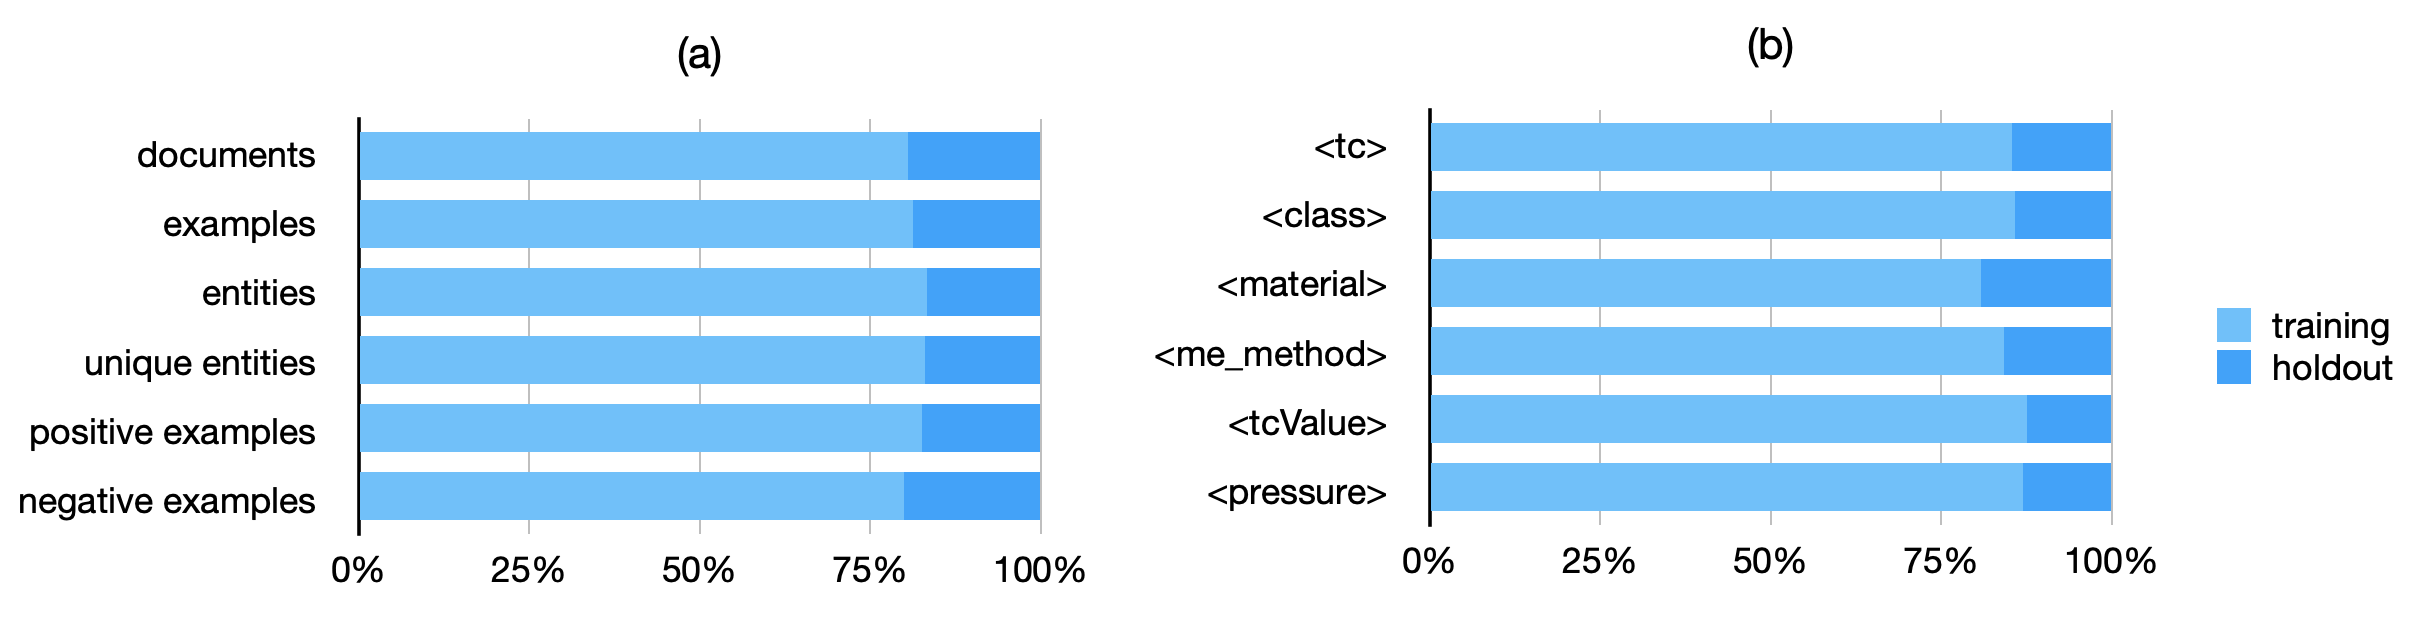
\includegraphics[width=\textwidth]{figures/automatic_extraction_supercon/superconductor-holdout-training-set}
    \caption{Holdout/training set distribution for (a) general metrics and (b) entity labels; entities and unique entities indicate the number of labelled entities with and without value duplicates, respectively, and positive examples (+) and negative examples (-) indicate the number of sentences with at least one entity and with no entities, respectively.}
    \label{fig:training-holdout-set-distribution}
\end{figure}

\begin{figure}[ht]
    \centering
    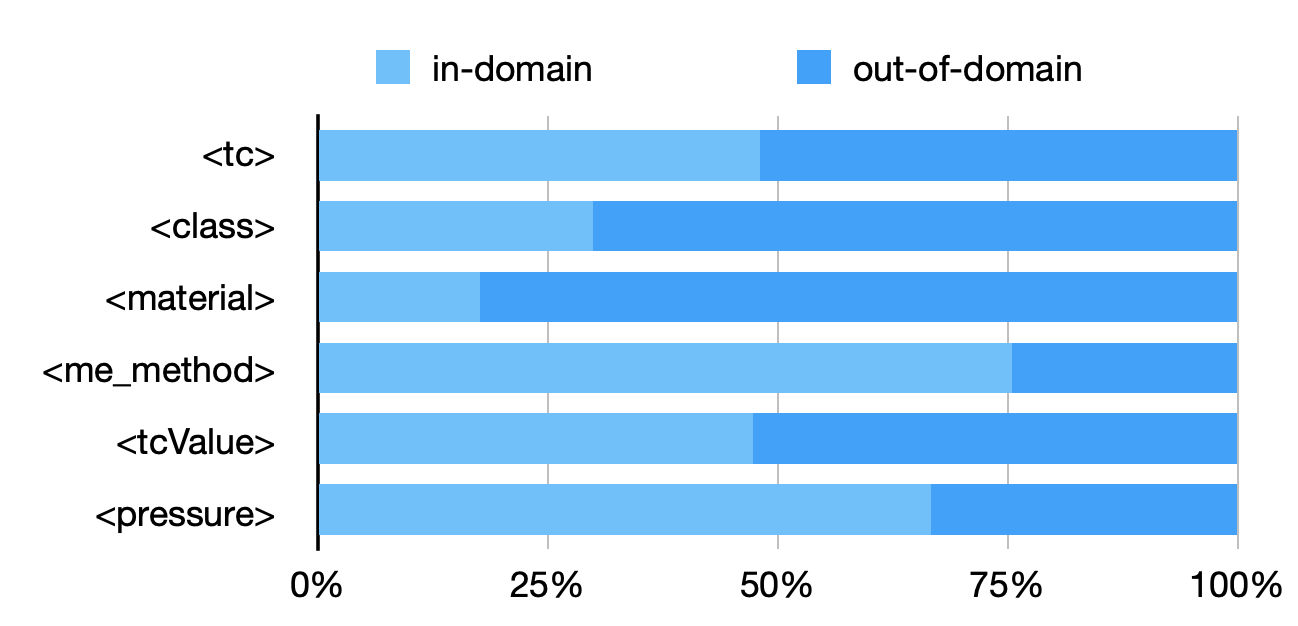
\includegraphics[width=0.6\textwidth]{figures/automatic_extraction_supercon/superconductor-out-domain-holdout-unique}
    \caption{Holdout ``out-of-domain'' rates. The entities from the holdout set that are also in the training set are ``in-domain'', and the entities that are not in the training set are ``out-of-domain''.}
    \label{fig:out-domain-holdout}
\end{figure}

We defined the ``out-of-domain'' ratio as the number of unique entities from the holdout set that were not in the training set.
The holdout set ``out-of-domain'' ratio was, on average, around 72\%, which challenges the model generalisation (every 100 entities in the holdout set, 72 were never seen before during training).
Most labels had an ``out-of-domain'' ratio above 50\%  (Figure~\ref{fig:out-domain-holdout});  \texttt{<material>}, the most important label, had the highest ratio (82\%) while \texttt{<me\_method>} and \texttt{<pressure>} have the lowest (25\% and 33\%). 
The low ratio of \texttt{<me\_method>} can be explained by their low entity variability (11.44\%).

\subsubsection{Results}
We evaluated each ML model by repeating the training and evaluation process five times (except for the CRF architecture, which is entirely predictable). Although the training and evaluation datasets are fixed, the way the training examples are provided to the model is randomly shuffled at each step, adding some entropy to the training, which is visible in the evaluation scores.
The results are then averaged as reported in Table~\ref{tab:evaluation-superconductors-ML-model}.

SciBERT obtained the best results with an F1 of 77.03\% and a recall of around 80.69\% (Table~\ref{tab:evaluation-superconductors-ML-model}).
The features did not improve RNN models: BidLSTM\_CRF and BidLSTM\_CRF\_FEATURES resulted in the same F1 score.
This result is a surprise because features such as superscript/subscript were expected to be determinants for recognising material sequences.


\begin{sidewaystable}[htbp]
    \centering\small
    \caption{Evaluation scores (\%) for the Superconductor ML model in the four architectures. For the DL architecture, the results are averaged over five runs. Support (Supp) indicates the number of labels in the training data. Values in bold indicate the highest score. P: precision, R: recall.}
    
    \scalebox{0.8}{
        \begin{tabular}{l ccc ccc ccc ccc r}
            \toprule
            \textbf{Label}        & \multicolumn{3}{c}{\textbf{CRF}} & \multicolumn{3}{c}{\textbf{BidLSTM\_CRF}} & \multicolumn{3}{c}{\makecell{\textbf{BidLSTM\_CRF}                                                                                                                                                 \\\textbf{\_FEATURES}}} & \multicolumn{3}{c}{\textbf{SciBERT}} & \textbf{Supp} \\
            \cmidrule(lr){2-4}\cmidrule(lr){5-7}\cmidrule(lr){8-10}\cmidrule(lr){11-13}\cmidrule(lr){14-14}
                                  & \textbf{P}                       & \textbf{R}                                & \textbf{F1}                                        & \textbf{P} & \textbf{R} & \textbf{F1}    & \textbf{P}     & \textbf{R} & \textbf{F1}    & \textbf{P} & \textbf{R}     & \textbf{F1}    &      \\
            \midrule
            \texttt{<class>}      & 79.74                            & 66.79                                     & 72.69                                              & 79.01      & 72.62      & \textbf{75.66} & 77.84          & 72.40      & 74.97          & 72.95      & 75.28          & 74.09          & 1646 \\
            \texttt{<material>}   & 79                               & 72.15                                     & 75.42                                              & 79.25      & 76.94      & 78.06          & 81.07          & 75.10      & 77.94          & 80.15      & 81.42          & \textbf{80.77} & 6943 \\
            \texttt{<me\_method>} & 60.25                            & 68.73                                     & 64.21                                              & 56.41      & 79.49      & 65.92          & 55.86          & 80.45      & 65.90          & 56.26      & 81.52          & \textbf{66.56} & 1883 \\
            \texttt{<pressure>}   & 46.15                            & 29.27                                     & 35.82                                              & 49.45      & 58.05      & 52.53          & 50.25          & 60.49      & \textbf{54.36} & 41.72      & 52.68          & 46.51          & 274  \\
            \texttt{<tc>}         & 84.36                            & 83.57                                     & \textbf{83.96}                                     & 78.61      & 82.54      & 80.48          & 79.19          & 82.07      & 80.60          & 74.46      & 82.66          & 78.35          & 3741 \\
            \texttt{<tcValue>}    & 69.8                             & 66.24                                     & 67.97                                              & 70.36      & 75.16      & 72.67          & 68.95          & 76.56      & 72.52          & 70.90      & 79.74          & \textbf{75.06} & 1099 \\
            \midrule
            All (micro avg)       & 76.88                            & 72.77                                     & 74.77                                              & 74.59      & 77.67      & 76.09          & \textbf{75.17} & 76.79      & 75.96          & 73.69      & \textbf{80.69} & \textbf{77.03}        \\
            \bottomrule
        \end{tabular}
    }
    
    \label{tab:evaluation-superconductors-ML-model} 
\end{sidewaystable}

The \texttt{<pressure>} label had the lowest performance scores in all architectures. We believe that 274 training examples are not sufficiently large. 
Pressure expressions depend on the context and the property they refer to, so in many occurrences, they may refer to different types of pressure (e.g., annealing pressure).
The label with the highest score was \texttt{<material>}, with F1 values of 80.77\% and 78.06\% for SciBERT and BidLSTM\_CRF, respectively. In addition, \texttt{<material>} had the highest ``out-of-domain'' ratio in the holdout set (greater than 75\%, Figure~\ref{fig:out-domain-holdout}) and the highest ``label variability'' (the ratio between unique entities and total entities, about 42\%), which suggests that the model recognises correctly materials that have not been ``seen'' during the training.
On the other hand, the \texttt{<me\_method>} label, which has lower ``label variability'' (around 11\%) and a low ``out-of-domain'' ratio, had an F1 score of 66.56\% with SciBERT and 65.92\% with BidLSTM\_CRF.
For \texttt{<tc>}, the CRF outperformed the other architectures (F1 score of 83.96\%), especially SciBERT (78.35\%). 
This outcome can be explained by the extremely low variability (12.69\%) of entities labelled as \texttt{<tc>}.

\begin{figure}[htbp]
    \centering
    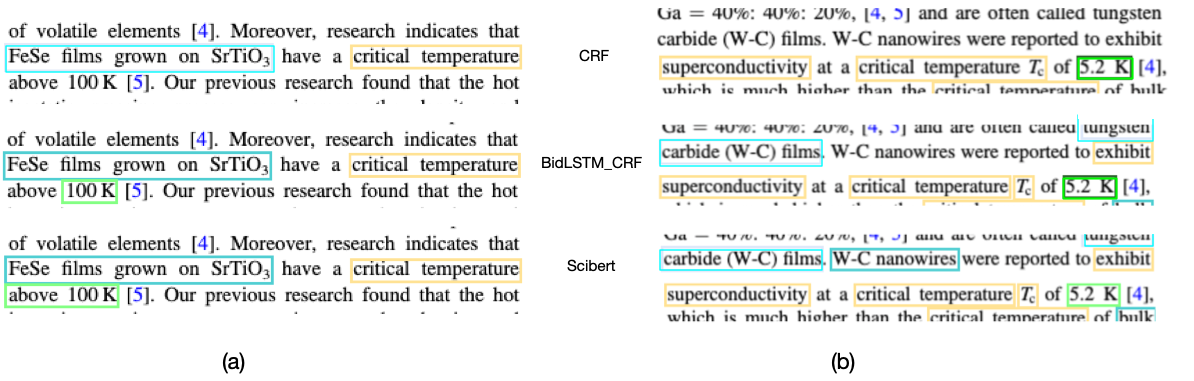
\includegraphics[width=\textwidth]{figures/automatic_extraction_supercon/example-comparison-archs.png}
    \caption{Examples taken from two sources~\cite{Gajda_2016, Shibata_2016} of results from three different architectures: CRF, BidLSTM\_CRF and, SciBERT. The boxes annotating the text represent the extracted entities (material are indicated in light blue, \tc~in green, and \tc~expressions in yellow).}
    \label{fig:example-comparison-architectures}
\end{figure}

SciBERT shows good generalisation capacity for unseen examples or examples appearing in different contexts.
For example, in Figure~\ref{fig:example-comparison-architectures}a, only SciBERT correctly extracts ``above 100K'', while CRF misses it entirely and BidLSTM\_CRF misses ``above''.
In the training data, ``above 100K'' is not present, but ``below 100K'' and ``\~100K'' are present, and several other entities contain the token ``above'', and SciBERT can understand that the token ``above'' is relevant to the temperature.
In a second example (Figure~\ref{fig:example-comparison-architectures}b), only SciBERT can correctly extract ``W-C nanowire'', which is not contained in the SuperMat training data.
Unfortunately, we cannot check whether ``above 100K'' or ``W-C nanowire'' are also present in the dataset used in the pre-train of SciBERT by their authors~\cite{Beltagy2019SciBERT} because the data are not available.


\subsection{Material parser segmentation model}

We trained the Material ML model using the second layer annotation set from SuperMat comprising entities of type \texttt{<material>}.
The resulting entities are segmented into eight pieces of information illustrated in Table~\ref{tab:material-parser-entities}.
We trained the same architecture in the same way as the ``Superconductors ML model''.

\subsubsection{Experimental settings}

In this model, we created an independent holdout set because manual annotation is performed on smaller chunks of text and requires less effort than annotating entire sentences.
We used material data extracted from a dataset of 500 documents (``500-papers'') from three publishers: \textit{American Institute of Physics} (AIP), \textit{American Physical Society} (APS) and \textit{Institute of Physics} (IOP)~\cite{foppiano2019proposal}.

\begin{figure}[ht]
    \centering
    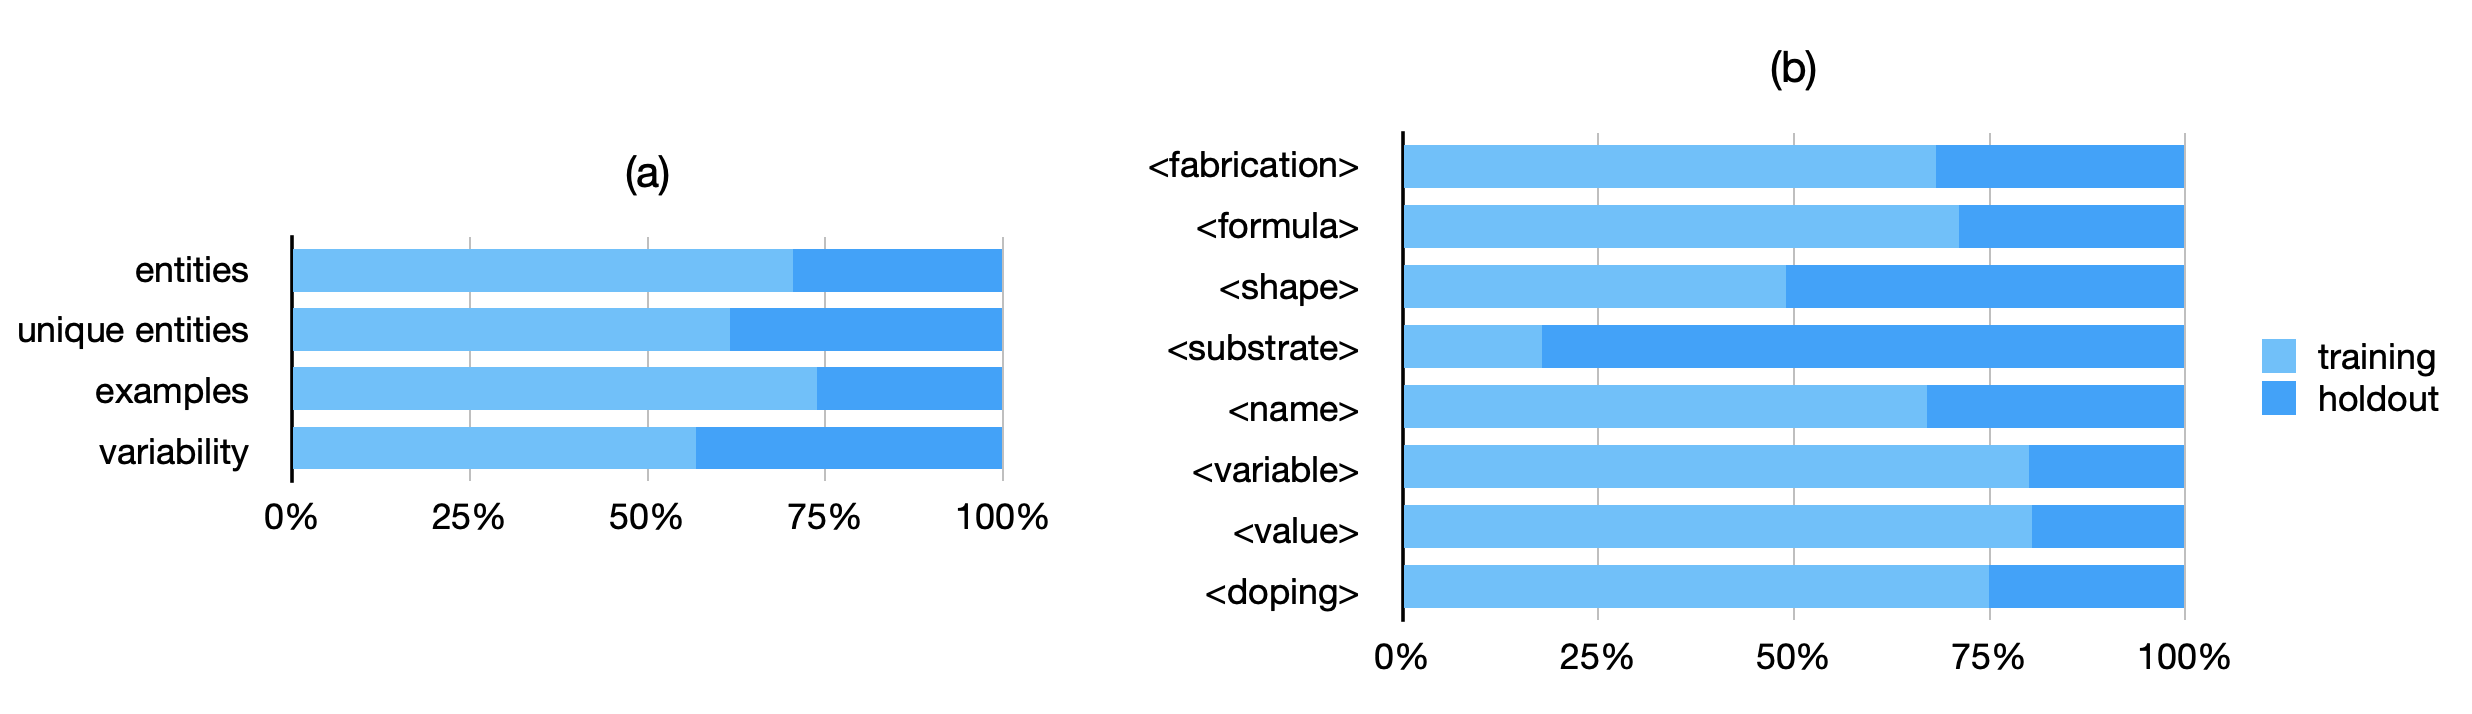
\includegraphics[width=\textwidth]{figures/automatic_extraction_supercon/material-holdout-training-set}
    \caption{Holdout/training set for the Material ML model: (a) general metrics and (b) entity labels.}
    \label{fig:material-training-holdout-set-distribution}
\end{figure}

The resulting holdout set has an average coverage greater than 25\% (Figure~\ref{fig:material-training-holdout-set-distribution}) and an average ``outside the domain'' ratio of 83.93\% (Figure~\ref{fig:material-out-domain-holdout}).

\begin{figure}[ht]
    \centering
    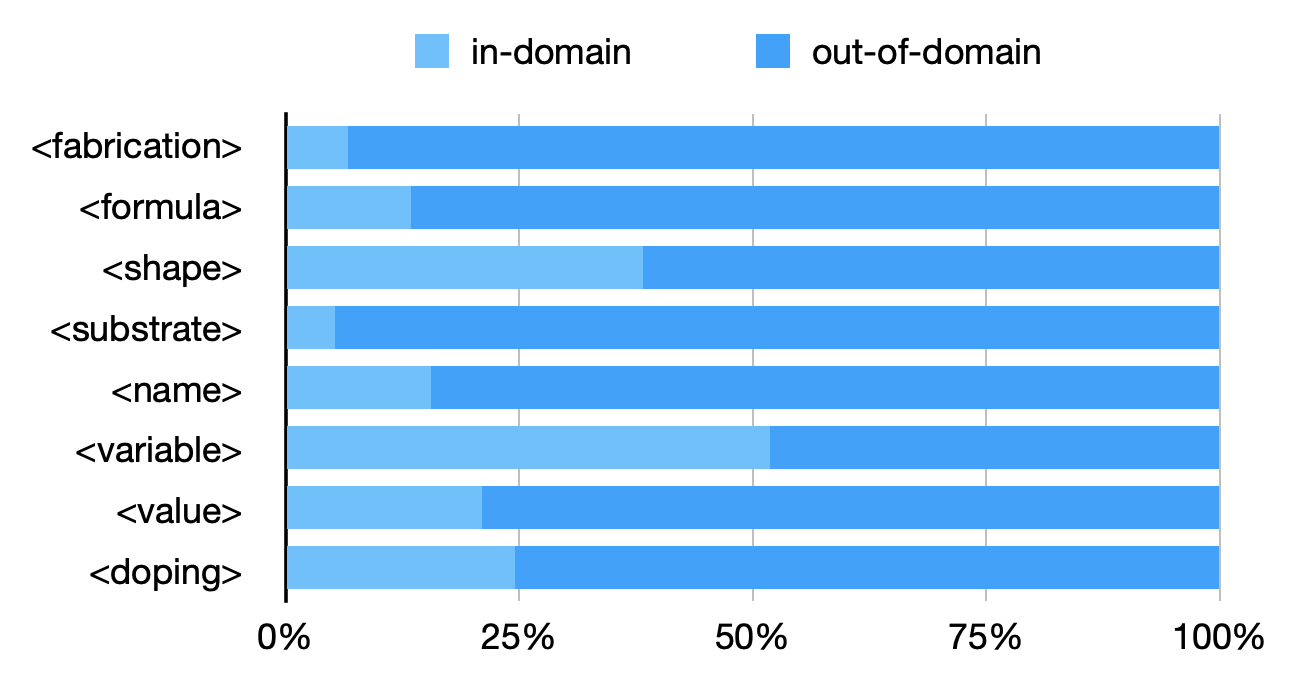
\includegraphics[width=0.6\textwidth]{figures/automatic_extraction_supercon/material-out-domain-holdout-unique}
    \caption{Holdout ``out-of-domain'' rates for the Material ML model. The entities from the holdout set that are also in the training set are the in-domain, and the entities that are not in the training set are the out-of-domain.}
    \label{fig:material-out-domain-holdout}
\end{figure}


\begin{table}[ht]
    \centering
    \caption{Holdout/Training set distribution (\%) between training and holdout sets for the Superconductor ML model. Positive examples indicate the number of sentences with at least one entity, and negative examples the number of sentences with no entities.}
    \begin{tabular}{lccc}
        \toprule
                                      & \textbf{training} & \textbf{holdout} & \textbf{\% holdout/training} \\
        \midrule
        \textbf{documents}         & 132               & 32               & 24.24\%                   \\
        \textbf{examples}          & 16902             & 3905             & 23.10\%                   \\
        \textbf{entities}          & 15586             & 3112             & 19.97\%                   \\
        \textbf{unique entities}   & 6699              & 1372             & 20.48\%                   \\
        \textbf{positive examples} & 8380              & 1776             & 21.19\%                   \\
        \textbf{negative examples} & 8522              & 2129             & 24.98\%                   \\
        \bottomrule
    \end{tabular}
    
    \label{tab:training-holdout-set-distribution-annex}
\end{table}

\begin{table}[ht]
    \centering
    \caption{Holdout/Training set distribution (\%) between training and holdout sets on different labels for the Superconductors ML model.}
    \begin{tabular}{lccc}
        \toprule
        label                 & \textbf{training} & \textbf{holdout} & \textbf{\% holdout/training } \\
        \midrule
        \texttt{<tc>}         & 3741              & 639              & 17.08\%                    \\
        \texttt{<class>}      & 1646              & 271              & 16.46\%                    \\
        \texttt{<material>}   & 6943              & 1649             & 23.75\%                    \\
        \texttt{<me\_method>} & 1883              & 355              & 18.85\%                    \\
        \texttt{<tcValue>}    & 1099              & 157              & 14.29\%                    \\
        \texttt{<pressure>}   & 274               & 41               & 14.96\%                    \\
        \bottomrule
    \end{tabular}
    \label{tab:training-holdout-labels-distribution-annex}
\end{table}

\begin{table}[htbp]
    \centering
    \caption{Holdout/Training set distribution (\%) training and holdout sets for the Material ML model.}
    \begin{tabular}{lccc}
        \toprule
                                    & \textbf{training} & \textbf{holdout} & \textbf{\% holdout/training} \\
        \midrule
        \textbf{examples}        & 13648             & 5728             & 41.97\%                   \\
        \textbf{entities}        & 4512              & 2817             & 62.43\%                   \\
        \textbf{unique entities} & 9268              & 3292             & 35.52\%                   \\
        \bottomrule
    \end{tabular}
    \label{tab:training-holdout-set-material-distribution-annex}
\end{table}

\begin{table}[htbp]
    \centering
    \caption{Holdout/Training set distribution (\%) training and holdout sets on different labels for the Material ML model.}
    \begin{tabular}{lccc}
        \toprule
        label                  & \textbf{training} & \textbf{holdout} & \textbf{\% holdout/training } \\
        \midrule
        \texttt{<fabrication>} & 94                & 44               & 46.81\%                    \\
        \texttt{<formula>}     & 6301              & 2569             & 40.77\%                    \\
        \texttt{<shape>}       & 809               & 841              & 103.96\%                   \\
        \texttt{<substrate>}   & 32                & 148              & 462.50\%                   \\
        \texttt{<name>}        & 1930              & 949              & 49.17\%                    \\
        \texttt{<variable>}    & 1795              & 449              & 25.01\%                    \\
        \texttt{<value>}       & 1895              & 463              & 24.43\%                    \\
        \texttt{<doping>}      & 792               & 265              & 33.46\%                    \\
        \bottomrule
    \end{tabular}
    \label{tab:training-holdout-labels-material-distribution-annex}
\end{table}


\subsubsection{Results}

SciBERT obtained the best results, with F1 at 84.15\% (Table~\ref{tab:evaluation-10fold-material-parser}).
The inclusion of features in the BidLSTM\_CRF architecture only improved the results by less than 1\% (from 83.13 to 83.76\%).
The label \texttt{<fabrication>} did not perform well in any architecture, most likely because it is too generic (Table~\ref{tab:material-parser-entities}), and the content is too heterogeneous. Another label, \texttt{<substrate>} has only one-third of the training examples of \texttt{<fabrication>} but obtained results that were three times higher with SciBERT, suggesting that \texttt{<fabrication>} should be split into separate and more homogeneous labels.

\begin{sidewaystable}[htbp]
    \centering\small
    \caption{Evaluation scores (\%) of the Material ML model with holdout set. Support (Supp) indicates the number of labels in the training data. Values in bold indicate the highest score. P: precision, R: recall.}

    \scalebox{0.9}{
    \begin{tabular}{l ccc ccc ccc ccc r}
        \toprule
        \textbf{Label}         & \multicolumn{3}{c}{\textbf{CRF}} & \multicolumn{3}{c}{\textbf{BidLSTM\_CRF}} & \multicolumn{3}{c}{\makecell{\textbf{BidLSTM\_CRF}                                                                                                                                                 \\\textbf{\_FEATURES}}} &  \multicolumn{3}{c}{\textbf{SciBERT}} & \textbf{Supp}  \\
        \cmidrule(lr){2-4}\cmidrule(lr){5-7}\cmidrule(lr){8-10}\cmidrule(lr){11-13}\cmidrule(lr){14-14}
                               & \textbf{P}                       & \textbf{R}                                & \textbf{F1}                                        & \textbf{P} & \textbf{R} & \textbf{F1}    & \textbf{P}     & \textbf{R} & \textbf{F1}    & \textbf{P} & \textbf{R}     & \textbf{F1}    &      \\
        \midrule
        \texttt{<doping>}      & 60.41                            & 55.85                                     & 58.04                                              & 67.98      & 62.42      & 64.95          & 69.00          & 62.34      & \textbf{65.43} & 63.58      & 62.79          & 63.16          & 792  \\
        \texttt{<fabrication>} & 40.00                            & 4.55                                      & 8.16                                               & 23.61      & 5.91       & 9.24           & 37.33          & 9.09       & 14.48          & 22.51      & 13.18          & \textbf{16.52} & 94   \\
        \texttt{<formula>}     & 80.81                            & 82.29                                     & 81.54                                              & 82.59      & 84.14      & 83.35          & 83.83          & 85.14      & 84.47          & 84.53      & 86.56          & \textbf{85.53} & 6301 \\
        \texttt{<name>}        & 72.2                             & 63.75                                     & 67.71                                              & 76.29      & 78.76      & 77.43          & 74.51          & 80.38      & 77.33          & 77.18      & 81.86          & \textbf{79.44} & 1930 \\
        \texttt{<shape>}       & 90.89                            & 92.51                                     & 91.69                                              & 90.93      & 95.79      & \textbf{93.29} & 90.33          & 95.74      & 92.96          & 89.67      & 97.20          & 93.28          & 809  \\
        \texttt{<substrate>}   & 37.04                            & 6.76                                      & 11.43                                              & 54.31      & 32.43      & 40.44          & 60.08          & 33.38      & 42.82          & 56.32      & 41.22          & \textbf{47.59} & 32   \\
        \texttt{<value>}       & 80.21                            & 83.15                                     & 81.65                                              & 84.81      & 89.33      & 86.99          & 85.16          & 90.15      & \textbf{87.58} & 83.14      & 85.92          & 84.50          & 1895 \\
        \texttt{<variable>}    & 96.85                            & 95.98                                     & 96.41                                              & 95.19      & 97.77      & 96.46          & 96.32          & 97.90      & \textbf{97.10} & 96.22      & 96.52          & 96.37          & 1795 \\
        \midrule
        All (micro avg)        & 81.15                            & 78.09                                     & 79.59                                              & 82.76      & 83.50      & 83.13          & \textbf{83.20} & 84.33      & 83.76          & 83.11      & \textbf{85.23} & \textbf{84.15} &      \\
        \bottomrule
    \end{tabular}
    }
    
    \label{tab:evaluation-10fold-material-parser}
\end{sidewaystable}

\subsection{RE evaluation}

This rule-based linking was evaluated using the linked entities from SuperMat~\cite{foppiano2021supermat} (Table~\ref{table:evaluation-linking}) and is divided considering each link type.
The F1 score for the \texttt{material-tcValue} relation was about 80\% with a precision of 88.40\%. 
\texttt{tcValue-pressure} F1 score was 3\% lower than  \texttt{material-tcValue} considering much less data available (support was 118 compared with 726).


\begin{table}[htbp]
    \centering
    \caption{Evaluation scores for the Linking. Support (Supp) indicates the number of labels in the training data. Values in bold indicate the highest score. P: precision, R: recall.}
    \begin{tabular}{lcccc}
        \toprule
        \textbf{Relationship type}          & \textbf{P} & \textbf{R} & \textbf{F1-} & Supp \\
        \midrule
        \textbf{material-tcValue}   & 88.40              & 74.52           & 80.87             & 726     \\
        \textbf{tcValue-pressure}   & 85.71              & 71.52           & 77.98             & 118     \\
        \textbf{me\_method-tcValue} & 62.28              & 65.74           & 63.96             & 151     \\
        \bottomrule
    \end{tabular}

    \label{table:evaluation-linking}
\end{table}



\subsection{End to end evaluation}
\label{sec:end2end}
End-to-end evaluation (E2EE) measures the system's capacity from the PDF documents until the final linked results.
We limited the scope of the E2EE to the triplet `material-\tc-pressure', which, at the moment, is the backbone upon which the database is built.
We performed the E2EE on the ``500-papers'' dataset where we manually examined the resulting database as follows: 1) we marked invalid records and 2) we identified the cause of failure from a predefined set of five \textit{error types} (Figure~\ref{fig:error-types}):
\begin{itemize}
    \item \textbf{From table}: the extracted text is wrongly extracted from a table. Although table content is ignored, the error rate from the Grobid library is still relevant due to the lack of training data.
    \item \textbf{Material-related NER}: entities are either not, wrongly, or partially recognised.
    \item \textbf{Properties NER}: quantity entities (pressure, temperature) are not correctly extracted. We measured this error separately to identify the failure that could be shared with the Quantity ML model.
    \item \textbf{\tc~classification}: the temperature is wrongly classified as superconducting \tc.
    \item \textbf{RE}: given the initial steps were performed correctly, the resulting entities are not linked correctly.
\end{itemize}

\begin{figure}[htbp]
    \centering
    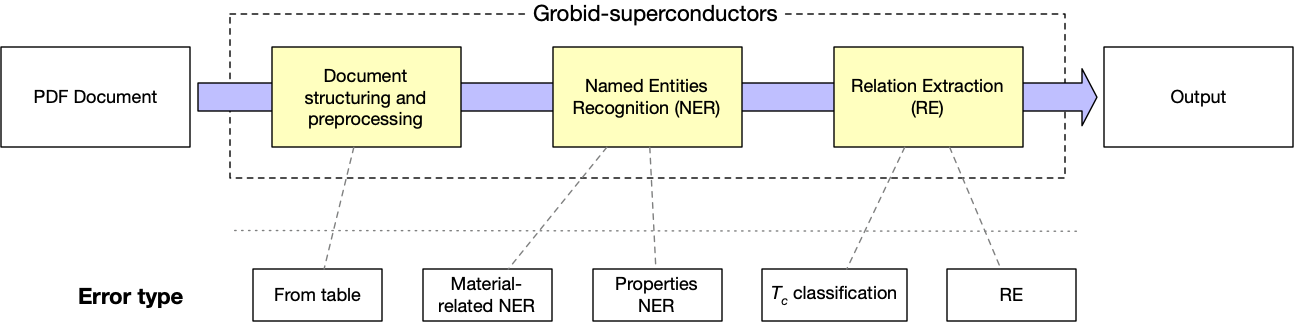
\includegraphics[width=\textwidth]{figures/automatic_extraction_supercon/error-types-colors}
    \caption{\textit{Error types} in the context of the data flow. }
    \label{fig:error-types}
\end{figure}

The E2EE scores are summarised in Table~\ref{table:end2end-evaluation-summary}.
The recall is omitted from the table because it is less relevant. However, we estimated that the recall is between 55\% and 60\%, considering a sample of articles. 
The precision score (micro average) was 72.60\% for all the subsections, although the precision of figure captions (59.28\%) and unknown subsections (57.14\%) were lower than those of the other subsections ($>$ 70\%).
The `unknown` subsections indicate that the extracted text's structure was not well identified by Grobid, but it was nonetheless aggregated.
The overall score increases to 73\% when excluding unknown subsections, 75.24\% when excluding figure captions, and 79.14\%  when excluding both.
Excluding these two subsections will not affect the amount of text because they account for less than 20\% of the total number of subsections.

\begin{figure}[htbp]
    \centering
    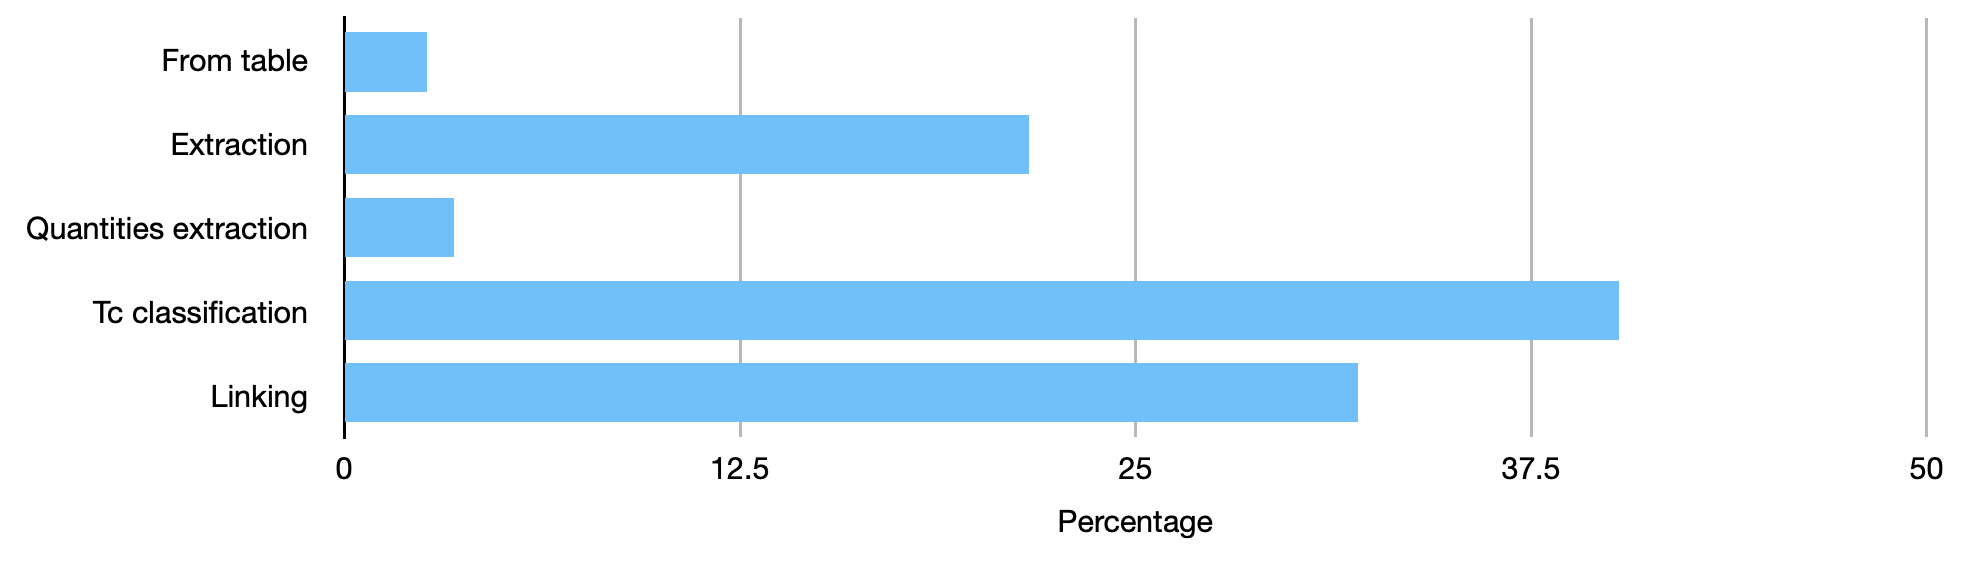
\includegraphics[width=\linewidth]{figures/automatic_extraction_supercon/error-types-bars-perc}
    \caption{Error type distribution in the E2EE of the \textit{500-papers} dataset.}
    \label{fig:error-types-distribution}
\end{figure}

The error types are summarised in Figure~\ref{fig:error-types-distribution}. The most common failures originate from \tc~classification (40\%), RE (32\%), and Material-related NER (20\%).
The most common \tc~classification failures are incorrect recognition of 1) relative values of \tc~(e.g., 1 K higher than material X); 2) values indicating the transition temperature width ($\Delta T_{c}$); 3) temperature values that are not \tc, for example, material synthesis temperatures ($T$), other critical transition temperatures that are not superconducting (e.g., $T_{Curie}$); and 4) values of temperature at which there is no superconductivity (e.g., ``at 70 K there is no superconductivity'').
``RE errors'' occur mainly when the text compares relative values of \tc~using materials as the basis for comparison (e.g., ``The Tc = 38 K is similar to the one of MgB$_{2}$'').
Finally, ``Material-related NER'' issues mainly originate from: 1) implicit mention of the base material when experimented using different ``substrates'' combination, and 2) mismatches between \texttt{<material>} and \texttt{<class>} which, by definition, overlap (see the SuperMat entities analysis in Section~\ref{automatic-corpus-analysis}).


\begin{table}[htbp]
    \centering
    \caption{Summary of the E2EE evaluation scores. Support indicates the number of labels in the training data.}
    \begin{tabular}{l c c}
        \toprule
        \textbf{Subsection}                                      & \textbf{Precision} & \textbf{Support} \\
        \midrule
        Title                                                    & 100                & 2                \\
        Abstract                                                 & 80.32              & 61               \\
        Paragraph                                                & 75.2               & 623              \\
        Figure captions                                          & 59.28              & 140              \\
        Unknown                                                  & 57.14              & 21               \\
        \midrule
        \textbf{Micro avg.}                                      & 72.60              & 847              \\
        \textbf{Micro avg.} (excl. figures)                      & 75.24              & 707              \\
        \textbf{Micro avg.} (excl. unknown sections)             & 73.00              & 603              \\
        \textbf{Micro avg.} (excl. figures and unknown sections) & 79.14              & 657              \\
        \bottomrule
    \end{tabular}
    
    \label{table:end2end-evaluation-summary}
\end{table}

\section{Conclusions}

This work introduces our proposed method for automatically extracting material-related expressions. This method is an essential component of our project, which aims to create a database of experimental data sourced from scientific literature.
We introduced four novelties: a high-quality dataset, SuperMat. The data was prepared using positive sampling, which increases recall in the output models. Each model was trained and evaluated among several architectures, of which the best performing were selected. Finally, we designed a 2-level process where a dedicated model parsed the material entities. 
We applied this specialised process in an unexplored area, where extracting information is challenging due to the intricate nature of the field and the specific attributes of the entities involved. 

The contribution described in this chapter has been published in the paper "Automatic extraction of materials and properties from scientific literature"~\cite{foppiano2023automatic} and partially (more details in Chapter~\ref{cha:measurements}) "Automatic identification and normalisation of physical quantities from scientific literature"~\cite{foppiano2019quantities}.


\chapter{SuperMat: Construction of a linked annotated dataset from superconductors-related publications}
\label{cha:supermat}
\section{Introduction}

In this contribution, we introduce SuperMat (Superconductor Materials), an annotated corpus of linked data derived from scientific publications on superconductors, which comprises 164 articles, 18698 entities, and 1524 links that are characterised into two layers. The first layer contains six categories: the names, classes, and properties of materials; links to their respective superconducting critical temperature (\tc); and parametric conditions such as applied pressure or measurement methods.
The second layer is dedicated to material entities and contains eight classes: formula, name, doping ratio, etc. 
The construction of SuperMat resulted from a fruitful collaboration between computer scientists and material scientists, and its high quality is ensured through validation by domain experts. 
The quality of the annotation guidelines was ensured by a satisfactory Inter Annotator Agreement (IAA) between the different annotators. 
SuperMat includes the dataset, annotation guidelines, and annotation support tools that use automatic suggestions to help minimise human errors.

\label{content-acquisition}
\section{Content acquisition}
SuperMat originates from PDF documents of scientific articles related to superconductor research. 
The original documents were collected from the following sources: (a) the Open Access (OA) version of peer-reviewed articles referenced in the SuperCon database records; 
(b) articles provided by domain experts containing suitable items and potential links of material names, \tc~values, measurement methods, and pressures; (c) articles from "condensed matter" category of arXiv (\url{https://arxiv.org/archive/cond-mat}) selected using the search terms of "superconductor", "critical temperature", and "superconductivity". 

Pre-print versions of peer reviewed articles were obtained using a bibliographic data lookup service called biblio-glutton (\url{https://github.com/kermitt2/biblio-glutton}) that aggregates data from various sources: the Crossref (\url{https://www.crossref.org/}) bibliographic database, the unPaywall (\url{http://unpaywall.org}) service, the PubMed Central repository (\url{https://pubmed.ncbi.nlm.nih.gov/}), and mappings to other databases. 
We queried \textit{biblio-glutton} using the bibliographic data of each article referenced in Supercon; subsequently, we downloaded the pre-print article associated with the retrieved record, if available. 
Although the published version may differ from the pre-print version of a document, the differences measured by comparing pre-print and peer-reviewed articles in biology~\cite{carneiro_comparing_2020} measured objective differences to be around 5\% %.


\section{Preliminary annotation study}
\label{subsec:preliminary-annotation-study}
A preliminary annotation study was carried out to assess the effort required from the annotators to reach an acceptable Inter Annotation Agreement (IAA \textgreater 0.7) .
We annotated two randomly selected OA papers, by using a preliminary version of the guidelines with a limited tag-set of four labels: \texttt{<material>}, \texttt{<tc>} (expression describing the presence or absence of superconductivity), \texttt{<tcValue>} (value of \tc), and \texttt{<doping>} (amount of substitution, such as stochiometric values, usually expressed as functions of x or y).
The process was iterated multiple times.
Each iteration ended with computing the IAA using the Krippendorff's alpha coefficient~\cite{Krippendorff2004ReliabilityIC,Zapf2016MeasuringIR}, while annotators discussed the disagreements, and updated the guidelines.

\begin{table}[htbp]
    \centering
    \caption{Summary of the IAA for each annotation iteration.}
    \begin{tabular}{ ccc } 
    \toprule
        \textbf{Iteration} \# & \textbf{IAA} & \textbf{IAA by label}  \\ [0.5ex] 
    \midrule
        1  & 0.45
        &\begin{tabular}{  cc  } 
            \texttt{<material>} & 0.45\\ 
            \texttt{<tc>} & 0.56\\
            \texttt{<tcValue>} & 0.50\\
            \texttt{<doping>} & 0.21\\
        \end{tabular}    
        \\ 
    \midrule
        2 & 0.65
        &\begin{tabular}{  cc  } 
            \texttt{<material>} & 0.75\\ 
            \texttt{<tc>} & 0.85\\
            \texttt{<tcValue>} & 0.85\\
            \texttt{<doping>} & 0.39 \\
        \end{tabular}          
        \\ 
    \midrule
        3 & 0.89
        & \begin{tabular}{  cc  } 
            \texttt{<material>} & 0.89\\ 
            \texttt{<tc>} & 0.91\\
            \texttt{<tcValue>} & 0.88\\
            \texttt{<doping>} & 0.94\\
        \end{tabular}       
        \\ 
    \bottomrule
    \end{tabular}
    
    \label{table:summary-preliminary-annotation}
\end{table}

Based on the results in Table~\ref{table:summary-preliminary-annotation}, IAA reached a satisfactory level of around 0.9 after the third iteration. 
Although the average IAA reached 0.7 on three of the four labels in the second iteration, the average agreement was unsatisfactory. 
When analysing the disagreement, we noticed that the low score in the \texttt{<doping>} label was caused by a heavy overlap with the \texttt{<material>} label, which required a more precise definition in the guidelines. 

Based on this preliminary study, the following changes were implemented. 
(a) The label \texttt{<doping>} was merged under the \texttt{<material>} because, even with detailed documentation it was too difficult for humans to annotate them consistently.
(b) Three more labels were added: measurement methods and pressure (described as parametric conditions in relation to \tc), and class of materials. 

\section{Tag-set design}
The tag set (also referred to as \textit{labels}) represents the classes of entities and the type of links between them, which were designed to be extracted from the text (Figure~\ref{fig:example-annotations-and-links}).

% example-annotated-corpus-postprocess.png
\begin{figure}[htbp]
  \centering
  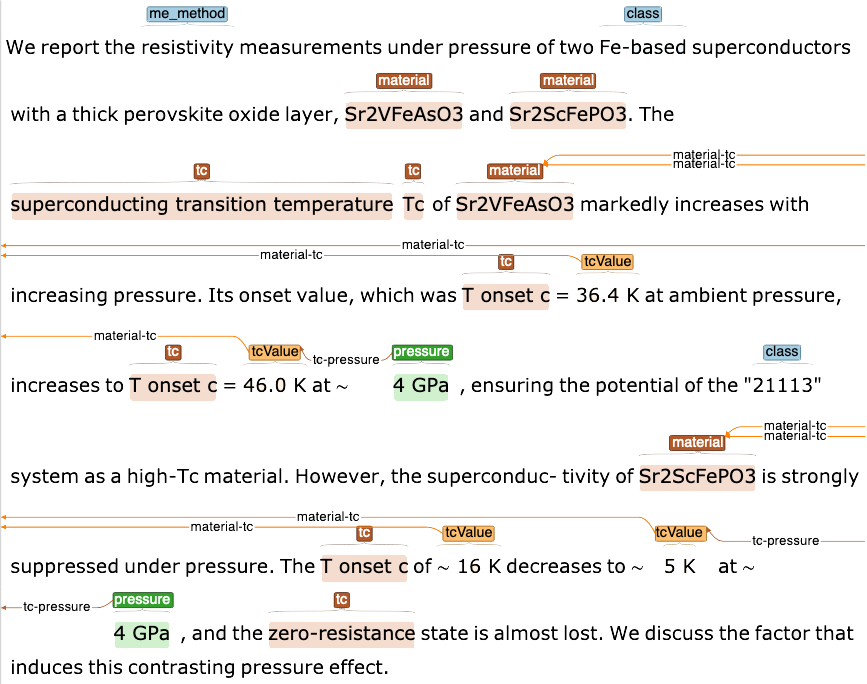
\includegraphics[width=\linewidth]{figures/supermat/Fig1.png}
  \caption{Example in the annotated corpus. Excerpt from © 2009 The Physical Society of Japan (J. Phys. Soc. Jpn. 78, 123707)}
  \label{fig:example-annotations-and-links}
\end{figure}


\subsection{Entities}
Entities (also referred to as Named Entities, mentions, or surface forms) are chunks of texts that represent information of interest, as follows: 

\paragraph{Class} (tag: \texttt{<class>}) represents a group of materials defined by certain characteristics.
Superconducting materials can be classified according to different criteria such as the composition and magnetic properties. 
Among publications collected for this study, the domain experts identified three types of classes based on: (a) the composition and crystal structure, (b) material phenomena (e.g. "I-type" and "II-type superconductivity", "BCS superconductors", "nematic", and "conventional/unconventional superconductivity"), and (c) high/low \tc~value (e.g. "high-tc” superconductors). 

In this work, we only considered the (a) classes, mainly because the material composition and crystal structure do not change with time. For example, a cuprate from 1998 is still called a cuprate today. 
In comparison, many material phenomena used for (b) are not robust enough and can be biased by the viewpoint of the author(s) or research group, or the measurement methods. 
Finally, the definition of "high-tc" superconductors (c) is completely relative; i.e., with the progress of research, materials once considered "high-tc" might not be so anymore.

\paragraph{Material} (tag: \texttt{<material>}) identifies the name of one or more materials. 
This label is used to collect the following types of information: 
\begin{itemize}
    \item Chemical formula indicating the material by its general or stochiometric formula (e.g. \texttt{LaFe\textsubscript{1-x}O\textsubscript{7}}, \texttt{WB\textsubscript{2}}),
    \item Compositional name (e.g. \texttt{magnesium diboride}) or abbreviations (e.g. \texttt{YBCO}), 
    \item The material's shape (e.g. wire, powder, thin film) or form of material (e.g. single/poly crystal), 
    \item Modification by a dopant (\texttt{Zn-doped}, \texttt{Si-doped}) or by percentage of doping (\texttt{2\%-doped}). We also considered qualitative expressions such as \textit{overdoped}, \textit{lightly doped}, and \textit{pure} as valid information, 
    \item Substrate information (e.g. \texttt{grown on MgO(100) film}) when it was adjacent to the material name or formula, in the text,
    \item Additional information about the sample (e.g. \texttt{as-grown}, \texttt{untwinned}, \texttt{single-layer}) when it was adjacent to the material name or formula, in the text. 
\end{itemize}

\paragraph{Superconducting critical temperature} (tag: \texttt{<tc>}) identifies expressions related to the phenomenon of superconductivity. Any temperature mentioned in the text is not necessarily the \tc. Rather, it could refer to the temperature for other processes/events such as annealing/sintering temperature, specific measurements, and structural changes.
This label identifies the presence or absence of superconductivity at a given temperature.
In addition, modifiers of this information (increasing/decreasing \tc) are also retained. 

\paragraph{Superconducting critical temperature value} (tag: \texttt{<tcValue>}) represents the temperature at which the superconducting phenomenon occurs. 
It can be defined by different experimental criteria, such as the onset, mid-point of resistivity drop, or zero resistivity.
This value also considers boundary conditions, such as the \textit{onset of superconductivity}, \textit{zero resistance}. 

\paragraph{Applied pressure} (tag: \texttt{<pressure>}) indicates the applied pressure corresponding to a measured \tc. 

\paragraph{Measurement method} (tag: \texttt{<me\_method>}) indicates the method used to measure or calculate the presence of superconductivity. Here, we considered the following categories: resistivity, magnetic susceptibility, specific heat, and theoretical calculations. 


\subsection{Relations}
\label{relations}
The relations connect entities of materials or samples to their corresponding properties, conditions, and results. 
The connecting links are non-directional, and each entity has no restrictions on the number of links. 
The relation types have been introduced in Section~\ref{subsec:re-solution}.


\subsection{Annotation guidelines}
\label{subsec:annotation-guidelines}
Annotation guidelines include the principles and the rules that describe what constitutes as desired information for the SuperMat dataset and how to annotate it. They include detailed descriptions of the specific rules that have been defined for each type of information to be annotated, with one or more definitions and examples illustrating what to annotate in different cases, exceptions, and references. We used an online system to track the discussions and decisions when a question or a comment was raised and provided a link to such issues in the respective description or example. 
In addition, the guidelines include \textit{linking rules} that provide information on how to connect the entities in a relationship correctly. 
The guidelines were built using a dynamic markup language (called RestructuredText) and stored in a git (\url{https://git-scm.com/}) version control system repository. We deployed them as HTML files via the web, which were updated automatically after each modification. They can be accessed at \url{https://supermat.readthedocs.io}.

\section{Annotation support tools}
\label{subsec:annotation-support-tool}
The task of annotating documents is tedious and requires both attention and subject knowledge from the annotators.
Annotation support tools aim to maximise the efficiency of annotators and minimise human mistakes. 
They comprise a web-based collaborative annotation tool, automatic annotation suggestions, and automatic corpus analysis. 

\subsection{Web-based collaborative annotation tool: INCEpTION}
\label{subsec:annotation-tool}

The annotation tool is the platform used for creating, correcting and linking annotations.
After evaluating several tools, we selected INCEpTION~\cite{tubiblio106270,eckart-de-castilho-etal-2016-web}, a web-based multi-user platform for machine-assisted rapid dataset annotation construction. 
INCEpTION provides supportive functionalities that include: 
\begin{itemize}
    \item Multi-layer annotation sheets allow different annotation schemas over the same documents, 
    \item Two annotation steps: annotation consists of manually correcting pre-imported documents, while curation allows another user to validate the annotations (Figure~\ref{fig:inception-curation-interface}). 
    \item On-the-fly automatic suggestions based on active learning and string matching (Figure~\ref{fig:inception-curation-interface}), 
    \item Bulk annotation corrections, and 
    \item Being open-source (Apache 2.0 license), and under active development at the time of this paper (\url{https://inception-project.github.io/}).
\end{itemize}

\subsection{Annotation suggestions}
\label{subsec:automatic-system-prototype}

Previous works have demonstrated that annotation suggestions improve the quality of the output~\cite{Fort2010InfluenceOP, Nvol2011SemiautomaticSA, Lingren2014EvaluatingTI}.
We provide two types of annotation suggestions. 
(i) \textit{Machine-based annotated data} that were assigned to the documents before loading into the annotation tool. Here, we use a machine learning (ML)-based system from a previously implemented prototype~\cite{foppiano2019proposal} to support our tag-set. 
(ii). \textit{Active learning recommendations} provided by INCEpTION are assigned on the fly based on previous annotations. 
The active-learning recommendations are less precise since they aim to increase the recall, and therefore they need to be explicitly accepted by the annotator.

\subsection{Automatic corpus analysis}
\label{automatic-corpus-analysis}
Automatic corpus analysis is a set of scripts designed to run after the validation step. 
These scripts automatically find inconsistencies in the links and entities, while extracting the statistics of the corpus. 
We calculated the inconsistencies by examining every annotated entity and computing the frequency of the same text being annotated with different labels. 
The script outputs a summary table by visualising each annotation value, as well as their labels and frequencies.
We visually inspected this table because the reported inconsistencies can be either obvious mistakes (Table~\ref{table:dataset-inconsistencies-clear}) or arise from ambiguities (Table~\ref{table:dataset-inconsistencies-unclear}); therefore, their context should be verified. 

\begin{table}[htbp]
    \caption{Statistical overview of the dataset. 
    Links\textsubscript{is} indicates the number of links within the same sentence (intra-sentence). Links\textsubscript{es} indicate the number of links from different paragraphs  (extra-sentence).  }
    \begin{tabular}{ m{6em}   m{4em}  m{6em}  m{7em}  m{6em} } 
    \toprule
        \multirow{2}{5em}{\textbf{Documents}} & \textbf{Files} & \textbf{Paragraphs} &	\textbf{Sentences} & \textbf{Tokens}\\
         & 164  &	2800 & 	20807 & 	1284569\\
    \midrule
        \multirow{2}{5em}{\textbf{Entities}} & \textbf{Entities} &  \multicolumn{2}{|c|}{\textbf{Unique entities}} &  \textbf{ Labels} \\
        & 18698 &  \multicolumn{2}{c}{8071} &  6 \\
    \midrule
        \multirow{2}{5em}{\textbf{Links}} & \textbf{Links} & \multicolumn{2}{|c|}{\textbf{Links\textsubscript{is}}} 
        & \textbf{Links\textsubscript{es}}\\
        & 1524  & \multicolumn{2}{c}{985} &	539	\\
    \bottomrule
    \end{tabular}
    \label{table:summary-content}
\end{table}

Although the links are conceptually non-directed, we have defined a practical convention to maintain their consistency. For example, \textit{material-tcValue} is always represented as a link between \texttt{<tcValue>} and \texttt{<material>} entities. 
The script also computes the statistics (Table \ref{table:summary-content}) for the number of entities (total, unique, by class), the number of links (total, intra- and inter-paragraph, between paragraphs), and other statistical information. 

\begin{table}[htbp]
    \centering\small
    \caption{Inconsistencies resulting from human mistakes.}
     
    \begin{tabular}{ ccccc } 
    \toprule
        Text & Label 1 & \# & Label 2 & \#\\
    \midrule
        \texttt{superconducting transition}     &   \texttt{<material>}   &    1   &   \texttt{<tc>}  &   61   \\
        \texttt{NCCO}    &	\texttt{<material>}   &    14   &   \texttt{<tc>}  &   1   \\
        \texttt{superconducting transition temperatures}     &   \texttt{<material>}   &    1   &   \texttt{<tc>}  &   11   \\
        \texttt{occurrence of superconductivity}    &	\texttt{<material>}   &    1   &   \texttt{<tc>}  &   1   \\
    \bottomrule
    \end{tabular}
    \label{table:dataset-inconsistencies-unclear}
\end{table}

\begin{table}[htbp]
    \centering\small
    \caption{Inconsistencies resulting from the overlapping of \texttt{<material>} and \texttt{<class>} labels.}
    \begin{tabular}{ ccccc } 
    \toprule
        Text & Label 1 & \# & Label 2 & \#\\
    \midrule
        \texttt{LiFeAs}         &   \texttt{<material>}   &    89   &   \texttt{<class>}  &   1   \\
        \texttt{Bi-2212}        &	\texttt{<material>}   &    34   &   \texttt{<class>}  &   1   \\
        \texttt{cobalt oxide}   &   \texttt{<material>}   &    89   &   \texttt{<class>}  &   1   \\
        \texttt{RE-123}         &	\texttt{<material>}   &    34   &   \texttt{<class>}  &   1   \\
    \bottomrule
    \end{tabular}
    \label{table:dataset-inconsistencies-clear}
\end{table}



\section{Annotation process}
\label{subsec:annotation-workflow}
The annotation workflow (Figure~\ref{fig:schema-comparison-modified-workflow}) was designed following the \textit{MATTER} (Model, Annotate, Train, Test, Evaluate, and Revise) schema\cite{pustejovsky2012natural} and other related work~\cite{Dieb2016, Krallinger2015TheCC}.
The workflow is composed of five steps (Figure~\ref{fig:schema-comparison-modified-workflow}): \textit{data-preparation}, \textit{correction}, \textit{validation}, \textit{testing and evaluation}, \textit{revision}. 
This workflow involves three main actors: the automatic process, computer scientists, and the domain experts.


% workflow-schema
\begin{figure}[htbp]
\centering
  \centering
  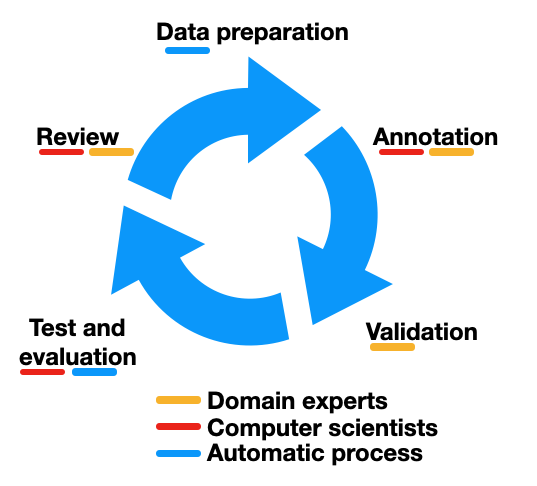
\includegraphics[width=0.5\linewidth]{figures/supermat/Fig2.png}
  \caption{Annotation workflow. Different colours illustrate the involvement of each group at each step of the workflow.}
  \label{fig:schema-comparison-modified-workflow}
\end{figure}

The first step of the annotation process involves preparing the machine-based annotated data from the source PDF documents. 
The PDF files are converted to an XML-based format, and annotation is automatically applied. 
This is followed by four more steps: 

\begin{itemize}
\item Annotation: The human annotator can select a document and manually add, remove, or modify each entity based on rules defined in the guidelines. Once the annotation is complete, the document is marked "ready" for the validation. 

\item Validation/Curation by domain experts: Annotations from different users are validated and merged into a final document (Figure~\ref{fig:inception-curation-interface}). 
The domain expert ("curator"), can compare the different annotated versions, and select the best combination of annotations, or add new ones. 
This step ensures that the annotations are cross-checked and that the document is validated by domain experts.

\item Automatic consistency checks and statistical analysis: This step aims to discover obvious mistakes such as mislabelling or incorrect linking. 
A sequence labelling model is trained and evaluated using 10-fold cross-validation. The evaluation provides precision, recall, and f-score metrics for all the labels.
The resulting model is used for producing machine-based annotated data in the following iteration.

\item Review: Retrospective analysis of the past iteration, where unclear cases are discussed and documented in the annotation guidelines. 

\end{itemize}

\section{Data transformation}
\label{subsec:transformation-of-data}
There are two processes of data transformation (Figure~\ref{fig:data-transformation}): (a) from the source document (PDF) to the dataset format representation (XML-based), and (b) from the dataset format representation to the annotation tool exchange formats (\url{https://inception-project.github.io/releases/0.16.1/docs/user-guide.html\#sect_formats}) and vice-versa. 

\begin{figure}[htbp]
    \centering
    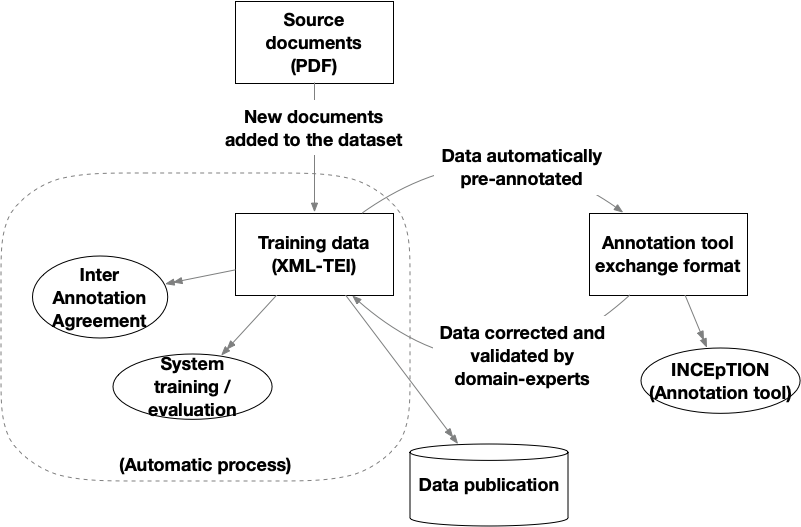
\includegraphics[width=\linewidth]{figures/supermat/Fig3.png}
    \caption{Summary of the data transformation flows.}
    \label{fig:data-transformation}
\end{figure}

\begin{itemize}
    \item PDF to XML-based: This step converts the PDF source document to the dataset format representation in XML following the Text Encoding Initiative (TEI, \url{https://tei-c.org/}) format guidelines. 
    Such transformation is performed by leveraging the functionalities provided by Grobid (\url{https://github.com/kermitt2/grobid}).
    
    We developed a customised process for collecting a subset of information from the source PDF document.
    The process extracts the title, keywords, and abstract from the header; and paragraphs, sections. and figure and table captions from the body.
    All the callouts to references, tables, and figures are ignored.
    The resulting structured document is then encoded in XML as will be described below. 
    \item XML to the annotation tool exchange formats: We transform our XML-formatted data into an INCEpTIONS compatible import format, such as the Webanno TSV 3.2 (\url{https://inception-project.github.io/releases/0.17.0/docs/user-guide.html\#sect_formats_webannotsv3}), and vice-versa using a set of Python scripts. 
    The Webanno TSV 3.2 format is an extension of the CONLL (\url{https://www.signll.org/conll/}) format, with additions of the header and column representation.
\end{itemize}

\section{Data Record}
\label{sec:data-record}
The dataset is composed of 164 PDF documents. Although we used the pre-print version of most of the articles to comply with copyright restrictions, the dataset cannot be distributed and is not publicly available in our repository. 
The three leading publishers represented in the corpus are the American Physical Society (APS), Elsevier, and IOP Publishing (Figure~\ref{fig:distribution-by-publisher}).
Figure~\ref{fig:distribution-by-year} illustrates the distribution by publication date.
We summarise SuperMat's content in Table~\ref{table:summary-content}, with the statistics of documents, entities, and links given separately. In particular, this dataset contains 16052 (7166 unique) entities spread over six labels and 1398 links. 

\begin{figure}[htbp]
\centering
\subfloat[Distribution by publisher.]{\resizebox*{8cm}{!}{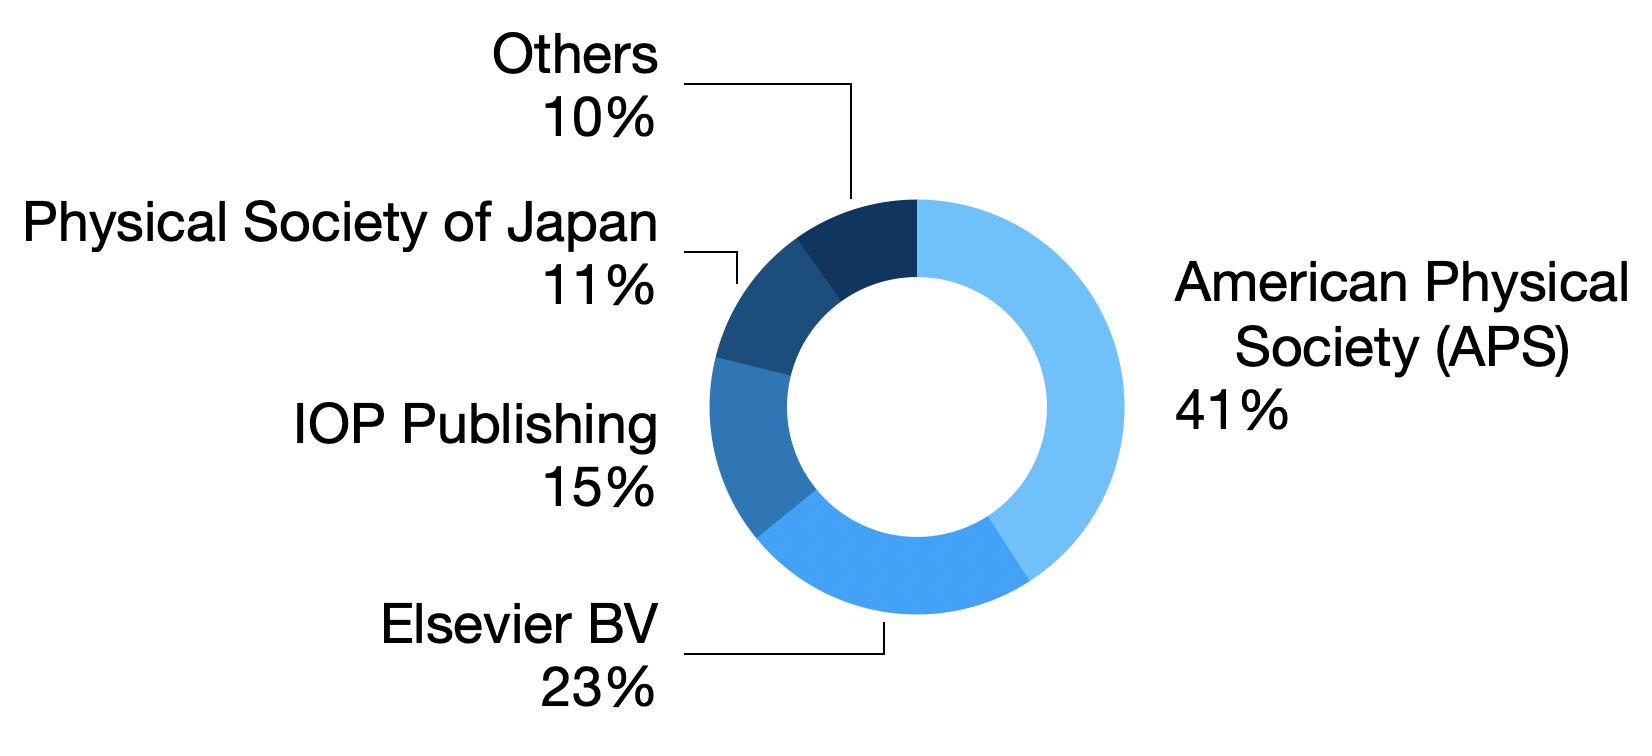
\includegraphics{figures/supermat/Fig5.png}}\label{fig:distribution-by-publisher}} 
\hspace{5pt} 
\subfloat[Distribution by year of publication.]{\resizebox*{6cm}{!}{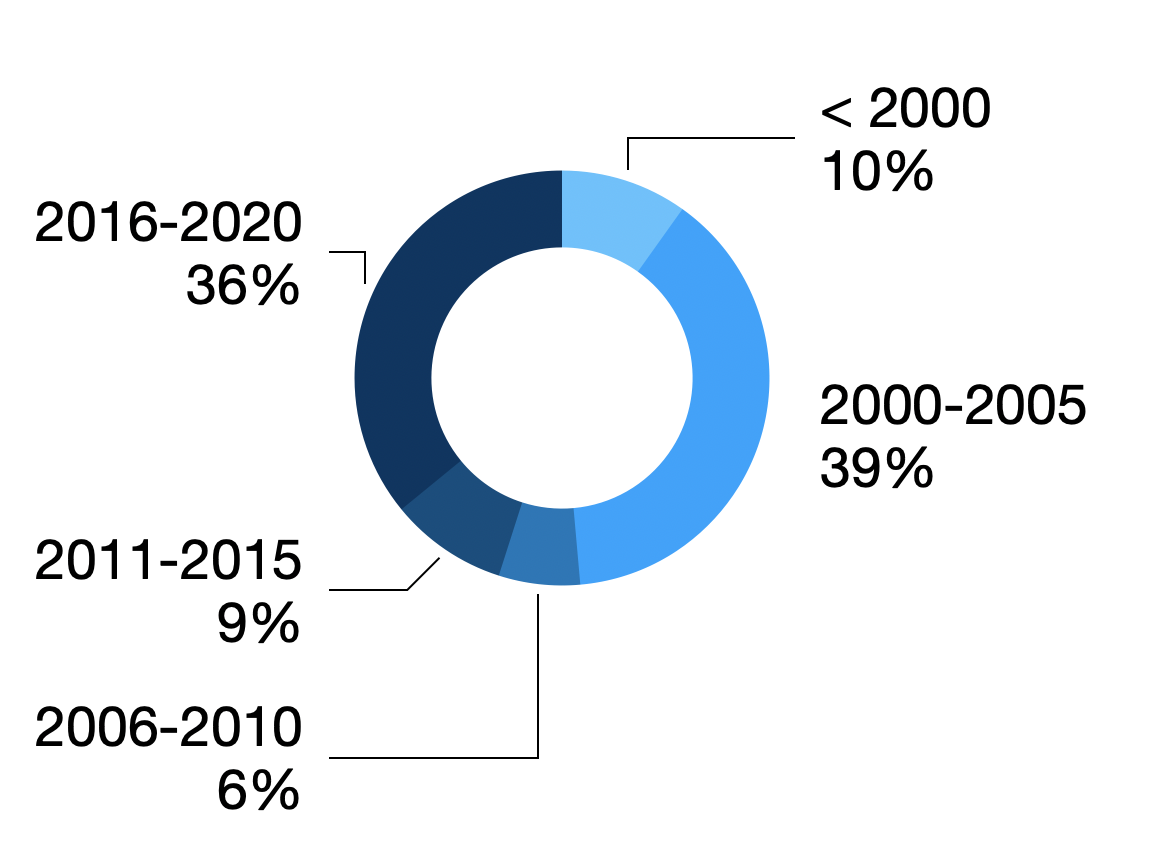
\includegraphics{figures/supermat/Fig6.png}}\label{fig:distribution-by-year}} 
\caption{Distribution of paper in the dataset by (a) publisher, and (b) year of publication.} 
\label{fig:dataset-distributions}
\end{figure}

Each document is encoded according to the XML TEI guidelines, which is a rich format for document representation. 
We have carried out no specific customisation, in order to remain fully compliant with the general TEI schema.
A TEI document has two main parts: the header (within the \texttt{<teiHeader>} tags) containing all the document metadata, and the body (within the section delimited by the \texttt{<text>} tag). 
The transformed data has the following structure: 

\begin{verbatim}
<TEI xml:lang="en" xmlns="http://www.tei-c.org/ns/1.0">
    <teiHeader>
        <fileDesc>
            <titleStmt>
                <title>[...]</title>
            </titleStmt>
            <publicationStmt>
                <publisher>[...]</publisher>
            </publicationStmt>
        </fileDesc>
        <encodingDesc/>
            <abstract>
                <p>[...]</p>
                <ab type="keywords">[...]</ab>
            </abstract>
        <profileDesc>
        </profileDesc>
    </teiHeader>
    <text>
        <body>
            <p>[...]</p>
            <ab type="tableCaption"> [...] </ab>
            <p> [...] </p>
            <ab type="figureCaption"> [...] </ab> 
        </body>
    </text>
</TEI>
\end{verbatim}

We transformed the source documents into these TEI-compliant structures using a simplified representation for specific content types.
The general objective is to flatten the content into a generic structure where priority is given to the annotations.
For instance, the keywords section, which groups together the key terms defined by the author(s) of the paper, is encoded using the generic tag \texttt{<ab type="keywords">} as free text, instead of the dedicated \texttt{<keywords>} element that would typically be part of the header. 
For both the abstract and the article body, the text is segmented in paragraphs (by means of the \texttt{<p>} element). 
The text is annotated with the generic \texttt{<rs>} (referencing string) element adorned with three attributes: \texttt{@type} (the entity type), \texttt{@corresp} (to provide a link to another annotation such as from \textit{material} to \tc~), and \texttt{@xml:id} (to uniquely identify the annotation for referencing or linking purposes).

Because only the captions of tables and figures are retained from the original source, a simplified encoding was defined by means of the \texttt{<ab>} element characterised by a \texttt{@type} attribute; that is, \texttt{<ab type="figureCaption">} for figure captions and \texttt{<ab type="tableCaption">} for table captions. 
Here is an example: 

\begin{verbatim}
<p>
    The electron-doped high-<rs type="tc">transition-
    temperature</rs> (<rs type="tc">Tc</rs>) <rs 
    type="class">iron-based pnictide</rs> 
    superconductor <rs type="material" 
    xml:id="m6">LaFeAsO1-xHx</rs> has a unique 
    phase diagram: Superconducting (SC) double domes are 
    sandwiched by antiferromagnetic phases at ambient 
    pressure and they turn into a single dome with 
    a maximum <rs type="tc">Tc</rs> that 
    <rs type="tcValue" xml:id="m7" 
    corresp="#m6,#9">exceeds 45K</rs> 
    at a pressure of <rs type="pressure" 
    corresp="#m7">3.0 GPa</rs>. 
    [...]
</p>
\end{verbatim}

In the above snippet, the entities \textit{"3.0 GPa"}, \textit{"exceed 45K"} and \textit{"LaFeAsO1-xHx"} are linked together via the pairs \texttt{@corresp, @xml:id}. 
This schema supports multiple annotations to any part of the document. 
For example, the entity \textit{exceed 45K} has a second link with the corresponding identifier (\textit{"\#9"}) to an annotation outside this paragraph.


\section{Practical applications}
The dataset was used in the following practical applications: 

\begin{itemize}
    \item Evaluation tasks: SuperMat has been used for evaluation of Large Language Models (LLM) in mining experimental data. In particular, NER and RE were tested and applied to the materials science literature~\cite{foppiano2024mining}. The dataset not being publicly available counted in a lower chance of being used for pre-training the LLM. 
    \item Automatic extraction: As discussed in Chapter~\ref{cha:extraction-experimental-data}, we used this dataset to develop a system for information extraction for superconducting materials.
    \item Weighted clustering was implemented using SuperMat annotations to identify research papers that discuss specific information of interest in different categories of superconducting materials. The annotations were used to bias the clustering algorithm towards entity similarity to achieve a more targeted clustering toward a specific type of information~\cite{dieb2022superconductor}.
\end{itemize}

\label{sec:technical-validation}
\section{Technical Validation} 
The following measures were employed to ensure the creation of a high-quality dataset: 
\begin{itemize}
    \item Each document was revised and validated by domain experts, 
    \item The workflow begins by assigning machine-based annotated data. This has demonstrated to improve the annotation task over several aspects, namely: time consumption, error rate, and annotation agreement~\cite{Fort2010InfluenceOP,Nvol2011SemiautomaticSA,Lingren2014EvaluatingTI}.
    \item On-the-fly automatic annotation recommendations, which provide fresh suggestions based on online decisions made by the annotators.
    \item The annotators have rapid access to changes in the annotation guidelines.
    \item The discussions were documented and linked in the guidelines. 
    \item Reviews are discussed and approved collaboratively between domain experts and other annotators.
\end{itemize}

\begin{table}[htbp]
    \centering
    \caption{Average IAA between the annotated and validated documents}
    \begin{tabular}{ c|c } 
    \toprule
        \textbf{Label} & \textbf{Average}\\
    \midrule
        \texttt{<material>}     &   0.956   \\
        \texttt{<me\_method>}   &	0.887   \\
        \texttt{<pressure>}     &	0.723   \\
        \texttt{<class>}        &	0.925   \\
        \texttt{<tcValue>}      &	0.863   \\
        \texttt{<tc>}           &	0.831   \\
    \midrule
        \textbf{Micro avg.}     &	0.911	\\
    \bottomrule
    \end{tabular}
    
    \label{table:average-iaa}
\end{table}

These guidelines are a vital piece of this work since they contain knowledge accumulated from these activities.
However, measuring the completeness of the guidelines is challenging. 
Assuming that the documents validated by domain experts represent the ground truth, we conducted IAA analysis between different annotators against the ground truth, using the Krippendorf's Alpha metric~\cite{Krippendorff2004ReliabilityIC}.
Table~\ref{table:average-iaa} shows the average IAA which is satisfying with a value of approximately 0.9. 
The highest score is obtained in the \texttt{<material>} entities, while the lowest one is obtained in \texttt{<pressure>}, which appears less frequently in the papers. 
The disagreement in \texttt{<tcValue>} can appear to be too low as compared with other labels such as \texttt{<class>}, which is, at first look, more ambiguous. 
We analysed the different cases and identified three reasons why this happens. 
First, \texttt{<tcValue>} may depend heavily on the context that requires more human attention, and it is therefore more prone to errors. 
Second, our suggestions system is challenged in its ability to disambiguate critical temperatures from other temperature data, leading to incorrect or invalid suggestions. 
Finally, the presence of mathematical symbols (e.g. "\texttt{\~}", "\texttt{<}", and "\texttt{>}") or other modifiers ("\texttt{up to}", "\texttt{exceeds}", etc.) before the \texttt{<tcValue>} could generate small disagreements that accumulate in the average score. 

\begin{table}[htbp]
    \centering
    \caption{Calculated IAA for annotations produced by domain experts, non-domain experts, and novices compared to the validated version. Annotations from domain experts are cross validated. }
    \begin{tabular}{ ccccc } 
    \toprule
        \textbf{Label} & \textbf{Domain experts} & \textbf{Non-domain experts} & \textbf{Novices}\\
    \midrule
        \texttt{<material>}     &   0.969   & 0.950    &   0.924   \\
        \texttt{<me\_method>}   &   0.890   & 0.862    &   0.901   \\
        \texttt{<pressure>}     &   0.836   & 0.741    &   0.746   \\
        \texttt{<class>}        &   0.990   & 0.836	   &   0.899   \\
        \texttt{<tcValue>}      &   0.895   & 0.734	   &   0.841   \\
        \texttt{<tc>}           &   0.874   & 0.776	   &   0.830   \\
    \midrule
        \textbf{All labels}        &	0.940   &   0.882	&      0.896   \\
    \midrule
        \textbf{\# paragraphs}  &   1066   &  1648	    &   325     \\
    \bottomrule
    \end{tabular}
   
    \label{table:comparison-iaa-nde-de}
\end{table}

To more precisely isolate the impact of the guidelines, we grouped the IAA results by level of domain experience. 
Table~\ref{table:comparison-iaa-nde-de} displays the IAA between the validated data and the data corrected by (a) domain experts (researchers who conduct superconducting development experiments), (b) non-domain-experts (researchers with no experience with superconducting materials), and (c) novices (students in materials science with limited domain experience). 
Obviously, the domain experts have the highest agreement and the IAA value (around 0.95) is 0.06 higher on average than that of non-domain experts. 
Thus, superconducting materials is a complex domain that requires knowledge in materials science to produce high-quality data, while crowdsourcing initiatives such as the Amazon Mechanical Turk might not work well. 

Furthermore, we measured the reliability of the guidelines by observing how quickly novices could reach a satisfying agreement with the validation of the domain experts, without any previous training on the guidelines.
From Table~\ref{table:comparison-iaa-nde-de}, the  novices can attain high IAA results by only using the guidelines and our annotation support tools. 
The average difference in agreement with domain experts (around 0.05) indicates that the guidelines are precise and complete, and that the annotations tools offer sufficient support. 

\section{Data Availability}
\label{sec:code-availability}
The references of the original papers and their bibliographical information, the annotation guidelines sources, and the developed code are available at the GitHub repository \url{https://github.com/lfoppiano/SuperMat}. The guidelines are freely accessible at \url{https://supermat.readthedocs.io}.
The data transformation scripts were written in Python and can be run from the command line. 
They require BeautifulSoup  (\url{https://www.crummy.com/software/BeautifulSoup/}), an open-source library for parsing XML and HTML formats. 
The data analysis scripts were developed as Jupyter notebooks (\url{https://jupyter.org/}) which can easily output results and graphs in the browser. 
The open source annotation tool is INCEpTION (\url{https://inception-project.github.io/}). 
The OA content was acquired using biblio-glutton (\url{https://www.github.com/kermitt2/biblio-glutton}). 
We computed the IAA using the Java library DkPro statistics (\url{https://dkpro.github.io/dkpro-statistics/})~\cite{Meyer2014DKProAA}.

% inception-curation-new.png
\begin{figure}[htbp]
    \centering
    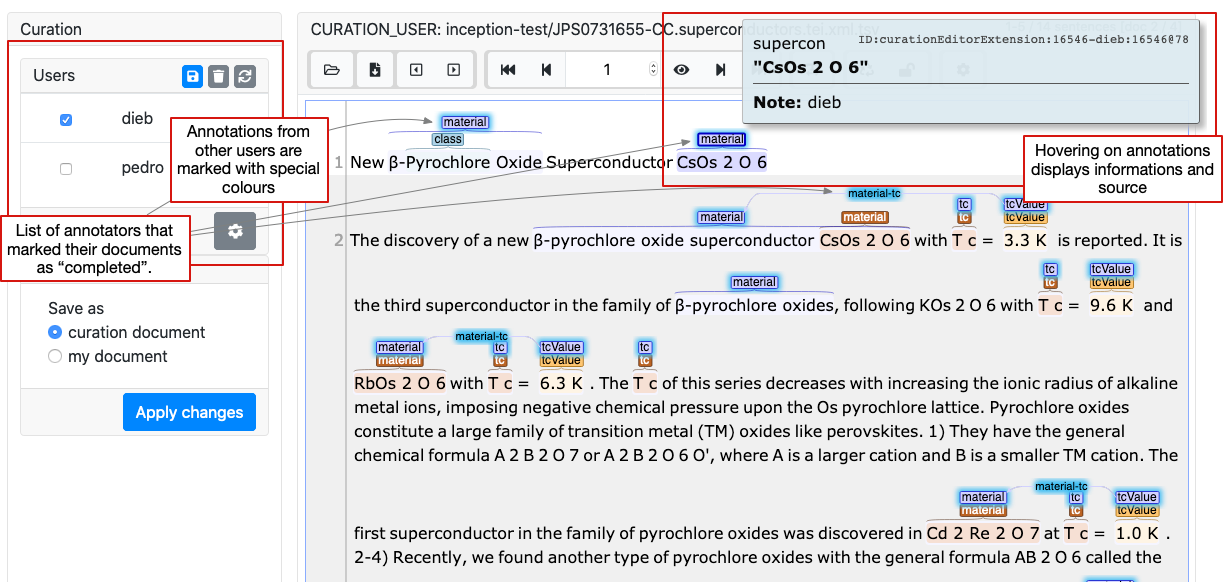
\includegraphics[width=\linewidth]{figures/supermat/Fig7.png}
    \caption{INCEpTION curation interface. Excerpt from © 2004 The Physical Society of Japan (J. Phys. Soc. Jpn. 73, 1655-1656)}
    \label{fig:inception-curation-interface}
\end{figure}


\section{Conclusions}
This chapter presents the process of creating an annotated linked dataset for scientific publications on the development of superconductors. SuperMat aims to create a reliable infrastructure for the improvement of text and data mining processes in the field of superconductor materials. We annotated 164 full-text articles using a two-layer set of annotations. The first layer contains six categories: the names, classes, and properties of materials; links to their respective superconducting critical temperature
(\tc); and parametric conditions such as applied pressure or measurement methods.
The second layer is dedicated to material entities and contains eight classes: formula,
name, doping ratio, etc.
Experts in the field have validated the dataset, which consists of 18698 top-layer entities, with 1524 links between materials, properties, and conditions.
This dataset is the building block for the contribution to material extraction (Chapter~\ref{cha:extraction-experimental-data}) presented in this dissertation. 

This contribution was published in the journal article "SuperMat: Construction of a linked annotated dataset from superconductors-related publications"~\cite{foppiano2021supermat}. 












\chapter{Extraction of properties and conditions as measurements of physical quantities}
\label{cha:measurements}
\section{Introduction}
% \section{Main contributions}
% \section{Experiments}
% \section{Conclusion}

In our approach to extracting material properties and conditions, we have opted for diverse components to accommodate the intricacies of different domains. 
For instance, we delve into critical temperature (Tc), applied pressure, and other pertinent factors in handling superconductor articles. 
Similarly, we focus on properties like coercivity and remanence when dealing with magnetic materials. 
This tailored approach is essential to capture domain-specific nuances effectively. However, we also recognise the necessity for a more generalised method alongside this specialised handling. Here, we prioritise a generic approach centred on extracting properties expressed through measurable physical quantities. This dual strategy ensures versatility in our material analysis framework while maintaining precision in capturing specific material behaviours across various domains.

For this task, we developed a Grobid module called Grobid-quantities that aims to provide a general solution to extracting quantities and physical measurements from the scientific literature. 
Grobid-quantities has been used in practical applications in other domains such as Earth observation data analysis~\cite{hundman2017measurement} 
It combines ML-based techniques and lexicon-based memory that aims to cover most of the existing units, unlike other work~\cite{aras2014applications}. 
Most other approaches lack the generalisation to an extensive corpus or deal mainly with specific languages. 
\cite{agatonovic2008large} addressed identifying the numeric properties of patents using GATE (General Architecture for Text Engineering). 
\cite{am2013processing} investigated issues applied to Russian-derived languages. \cite{berrahou2013extract} described an attempt to recognise units by looking up terms from an ontology, using ML combined with pattern matching and string metrics. 
At the time of development, other ML-based approaches were limited to certain fields~\cite{dieb2015framework} or domain~\cite{kang_extracting_2013}.
We incorporate a normalisation process to convert measurements to the base units of the international system (SI), a crucial step in harmonising data from various documents, disciplines and domains.

\section{Proposed solution}
\label{sec:system}

The system accepts input in text or PDF files similar to the approach described in Chapter~\ref{cha:pdf_extraction}. 
The extracted content is processed in three steps: (a) tokenisation, (b) extraction and parsing of measurements, and (c) normalisation of quantities.

\subsection{Data model}
\label{subsec:data-model}

The data model (Figure \ref{fig:data-model-schema-2}) was based on the concept of \textit{Measurement}, which links an object or a substance with one or more \textit{quantities}. 
We defined four \textit{Measurements} types: (a) atomic, in case of a single measurement (e.g., 10 grams). (b) interval (\textit{from 3 to 5 km}) and (c) range ($100 \pm 4$ mm) for continuous values, and (d) a list of discrete values. A \textit{Quantity} links the quantitative value and the unit. 

\label{subsub:data-model}
\begin{figure}[htbp]
  \centering
  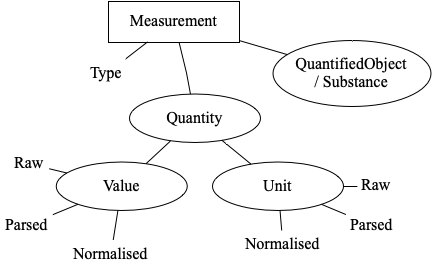
\includegraphics[width=0.8\linewidth]{figures/quantities/schema-2.png}
  \caption{Schema of the data model, from the data parsing and normalisation point of view.}
  \label{fig:data-model-schema-2}
\end{figure}

Since data extracted from PDF documents unavoidably present irregular tokens from incorrect UTF-8 encoding or missing fonts, we designed this model to allow partial results. 
The \textit{Value} and \textit{Unit} entities allow three different representations (Figure \ref{fig:data-model-schema-2}): \textit{Raw} as appear in the input, \textit{Parsed} unifies the value into the numerical expression, and the unit with its properties (system, type). Finally, \textit{Normalised} contains the transformed unit and values to the SI system. \textit{Value} object supports four types of representations: numeric (2, 1000), alphabetic (two, thousand), scientific notation ($3\cdot10\textsuperscript{5}$), and time, which is also an expression of measurement. Units objects are organised following the SI, which allows representing units as products of simpler compounds (e.g. m/s to $m \cdot s\textsuperscript{-1}$) further decomposed as triples (prefix, base and power).

\subsection{Tokenisation}
This process splits the input data into tokens. Grobid-quantities uses two-phase tokenisation: (1) first, it splits by punctuation marks, then (2) each resulting token is re-tokenised to separate adjacent digits and alphanumeric characters. Given the example \texttt{25m\^{}2}, first returns a list \texttt{[25m, \^{}, 2]} and then recursively divides \texttt{25m} as \texttt{[25, m]}  resulting in \texttt{[25, m, \^{}, 2]}.

\subsection{Extraction}
% Quantity model 
The tokens are passed through three ML models following the 2-level approach (Section~\ref{sec:two-levels-approach}): first, the \textit{Quantities} parser determines the appropriate unit and value tags. The results are further processed by the respective \textit{Units} and \textit{Values} parsers as illustrated in Figure \ref{fig:schema-cascade}.  

\begin{figure}[htbp]
  \centering
  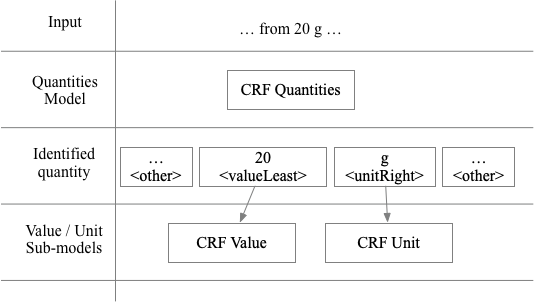
\includegraphics[width=\linewidth]{figures/quantities/schema-cascade}
  \caption{The cascade approach of the applied parsers. The Quantities parser recognises values and units passed to Values and Units parsers for further extraction.}
  \label{fig:schema-cascade}
\end{figure}

Table \ref{tab:quantities-model-labels} describes the labels predicted by \textit{Quantities} parser. Note that to reconstruct complex structured objects from the flat sequence generated by the engine, additional labels are necessary (such as \texttt{<unitLeft>}, \texttt{<unitRight>}, for units).

\begin{table}[htbp]
\centering
  \caption{Labels description for the Quantities parser. The values referred to by the label are highlighted in bold.}
  \label{tab:quantities-model-labels}
  \begin{tabular}{lll}
    \toprule
    Label & Description & Example\\
    \midrule
    \texttt{<valueAtomic>} & value of an atomic quantity & \textbf{2} m \\
    \texttt{<valueLeast>} & least value in an interval & from \textbf{2} m \\
    \texttt{<valueMost>} & max value in an interval & up to \textbf{7} m \\
    \texttt{<valueBase>} & base value in a range & $\textbf{20}\pm7$ m \\
    \texttt{<valueRange>} & range value in a range & $20 \pm \textbf{7}$ m \\
    \texttt{<valueList>} & list of quantities & \textbf{2}, \textbf{3} and \textbf{10} m \\
    \texttt{<unitLeft>} & left-attached unit & \textbf{pH} 2 \\
    \texttt{<unitRight>} & right-attached unit & 2 \textbf{m} \\
    \texttt{<other>} & everything else & - \\
  \bottomrule
\end{tabular}
\end{table}

% Gazetteers
Previous work presented extensive use of databases or ontologies. In our solution, we used a similar approach. We created a list of units (in English, French, and German) with their characteristics: system (SI base, SI derived, imperial, etc.) and type (volume, length, etc.) and their representations: notations (m\textsuperscript{3}, \texttt{m\^{}3}), lemmas (cubic meter, cubic metre) and inflexions (cubic meters, cubic metres). We made this list available through the \textit{Unit Lexicon}, which offers unit lookups by properties (such as notation, lemma, and inflexion). A second gazetteer was created to allow the transformation of alphabetic values into numeric ones (for example, 21 to 21).

Features in the \textit{Quantities} model are generated from preceding and following tokens, presence of capital, and digits. Orthogonal features are obtained through the \textit{Unit Lexicon}, like a \textit{Boolean} indicating whether a token is a known unit. Typographical information (format, fonts, subscript and superscript) are ignored. 

% Unit model 
The \textit{Units} parser works at the character level and uses the \textit{Unit Lexicon} to highlight known units or prefixes. The input tokens are parsed and transformed into a product of triples (prefix, base, power) as shown in Table \ref{tab:units-model-labels}. For example, \texttt{ Kg / mm\textsuperscript{2}}, corresponds to \texttt{$Kg\cdot mm\textsuperscript{-2}$} and becomes \texttt{[(K, g, 1), (m, m, -2)]} as a product of triples. We define "simple units" as all the units that can be decomposed in a single triplet and complex units when they are decomposed in multiple triplets. 

\begin{table}[htbp]
\centering
  \caption{Labels description for the Units parser. In bold are highlighted specific examples. }
  \label{tab:units-model-labels}
  \begin{tabular}{lll}
    \toprule
    Label & Description & Example\\
    \midrule
    \texttt{<prefix>} & prefix of the unit  & \textbf{k}m\textsuperscript{2} \\
    \texttt{<base>} & unit base & k\textbf{m}\textsuperscript{2}\\
    \texttt{<pow>} & unit power & km\textsuperscript{\textbf{2}}\\
    \texttt{<other>} & everything else & - \\
  \bottomrule
\end{tabular}
\end{table}

We then use the structured triples to fetch the corresponding information (system, type) from the \textit{Unit Lexicon} and attach them to the resulting object. 
This implementation processes the unit characters in right-to-left order. 
%Priority modifiers, such as parenthesis, are ignored because more complex to manage and not frequent. 
Priority modifiers, such as parentheses, are ignored. They are generally not frequent in unit expressions and require a more complex logic.

In parallel, the \textit{Values} parser unifies the format of the identified values into numerical formats. It supports four types: numeric, alphabetic, scientific notation, and time expression (see Table \ref{tab:values-model-labels}). Different techniques are applied for each type: alphabetic expressions are looked up in the word-to-number gazetteer, and scientific notation is parsed and calculated mathematically. Time expressions are further segmented using the Grobid built-in "Date" model.

\begin{table}[htbp]
\centering
  \caption{Labels description for the Values parser. In bold are highlighted specific examples.}
  \label{tab:values-model-labels}
  \begin{tabular}{lll}
    \toprule
    Label & Description & Example\\
    \midrule
    \texttt{<number>} & numeric value / coefficient & $\textbf{2.5}\cdot10\textsuperscript{\textbf{5}}$ \\
    \texttt{<alpha>} & alphabetic value & \textbf{twenty} \\
    \texttt{<time>} & time expression  & in \textbf{1970-01-02}\\
    \texttt{<base>} & base in scientific notation & $2.5\cdot\textbf{10}\textsuperscript{5}$\\
    \texttt{<pow>} & exponent in scientific notation & $2.5\cdot10\textsuperscript{\textbf{5}}$ \\
    \texttt{<other>} & everything else & - \\
  \bottomrule
\end{tabular}
\end{table}

\subsection{Normalisation}

The measurements extracted are transformed to the base SI unit (grams to kg, Celsius to Kelvin, etc.). We used an external Java library called Units of Measurement~\cite{units_of_measurement}, which provides a set of standard interfaces and implementations to handle units and quantities safely. Manipulating measurements with transformations often leads to common errors due to wrong rounding and approximations. 

\section{Evaluation and results}
\label{sec:results}

We trained and evaluated our system's models using a dataset based on 32 scientific publications (English, Open Access (OA)) and three patents (with translation in English, French, and German) randomly selected from different domains such as medicine, robotics, astronomy, and physiology. 
Training data was generated automatically and then corrected and cross-checked by three annotators. The dataset was then divided into a training set (26 documents) and an evaluation set (9 documents).
We used the holdout dataset partition to evaluate each model and produce precision, recall, and f1 scores, as summarised in Tables~\ref{tab:evaluation-quantities-holdout},~\ref{tab:evaluation-units-holdout}, and~\ref{tab:evaluation-values-holdout}. 
As presented in Chapter~\ref{cha:extraction-experimental-data}, we report the results of the three architectures introduced in Section~\ref{sec:ml-architectures}: CRF, RNN (with and without layout features), and transformers, fine-tuning a pre-trained SciBERT~\cite{Beltagy2019SciBERT}. 

\begin{table}[htbp]
    \centering\small
    \caption{Evaluation scores (\%) of the Quantities ML model with holdout set. Support (Supp) indicates the number of labels in the training data. Values in bold indicate the highest score. P: precision, R: recall. Deep learning results are averaged over five independent runs of training and evaluation. }

    \scalebox{0.6}{
    \begin{tabular}{l ccc ccc ccc ccc r}
        \toprule
        \textbf{Label}         & \multicolumn{3}{c}{\textbf{CRF}} & \multicolumn{3}{c}{\textbf{BidLSTM\_CRF}} & \multicolumn{3}{c}{\makecell{\textbf{BidLSTM\_CRF}                                                                                                                                                 \\\textbf{\_FEATURES}}} &  \multicolumn{3}{c}{\textbf{SciBERT}} & \textbf{Supp}  \\
        \cmidrule(lr){2-4}\cmidrule(lr){5-7}\cmidrule(lr){8-10}\cmidrule(lr){11-13}\cmidrule(lr){14-14}
                               & \textbf{P}                       & \textbf{R}                                & \textbf{F1}                                        & \textbf{P} & \textbf{R} & \textbf{F1}    & \textbf{P}     & \textbf{R} & \textbf{F1}    & \textbf{P} & \textbf{R}     & \textbf{F1}    &      \\
        \midrule
        \texttt{<unitLeft>} & 88.74 & 83.19 & 85.87 & 88.56 & 92.07 & 90.28 & 88.91 & \textbf{92.20} & 90.53 & \textbf{93.99} & 90.30 & \textbf{92.11} & 464 \\
        \texttt{<unitRight>} & \textbf{30.77} & 30.77 & 30.77 & 24.75 & \textbf{30.77} & 27.42 & 21.73 & 30.77 & 25.41 & 21.84 & \textbf{36.92} & \textbf{27.44} & 13 \\
        \texttt{<valueAtomic>} & 76.29 & 78.66 & 77.46 & 78.14 & 86.06 & 81.90 & 78.21 & 86.20 & 82.01 & \textbf{84.50} & \textbf{88.19} & \textbf{86.31} & 581\\
        \texttt{<valueBase>} & 84.62 & 62.86 & 72.13 & 83.51 & 94.86 & 88.61 & 83.36 & \textbf{97.14} & 89.72 & \textbf{100.00} & 90.86 & \textbf{95.20} & 35 \\
        \texttt{<valueLeast>} & 77.68 & 69.05 & 73.11 & \textbf{82.14} & 60.63 & 69.67 & 80.73 & 60.63 & 69.12 & 81.09 & \textbf{71.59} & \textbf{76.04} & 126 \\
        \texttt{<valueList>} & 45.45 & 18.87 & 26.67 & 62.15 & 10.19 & 17.34 & \textbf{73.33} & 8.68 & 15.33 & 64.12 & \textbf{43.78} & \textbf{51.64} & 53\\
        \texttt{<valueMost>} & 71.62 & 54.64 & 61.99 & 77.64 & 68.25 & 72.61 & 77.25 & \textbf{70.31} & 73.58 & \textbf{81.52} & 67.42 & \textbf{73.71} & 97\\
        \texttt{<valueRange>} & \textbf{100.00} & 97.14 & 98.55 & 96.72 & \textbf{100.00} & \textbf{98.32} & 94.05 & 98.86 & 96.38 & 99.39 & 91.43 & 95.24 & 35\\
        \midrule
        \textbf{All (micro avg.)} & 80.08 & 75 & \textbf{77.45} & 81.81 & 81.73 & 81.76 & 81.76 & 81.94 & 81.85 & \textbf{86.24} & \textbf{83.96} & \textbf{85.08} & \\
        \bottomrule
    \end{tabular}
    }
    
    \label{tab:evaluation-quantities-holdout}
\end{table}


% Scores + discussion Quantities model 
The best results of the Quantities ML models were achieved by the SciBERT model, for which we recorded an F1 micro-average of 85.14\% with precision and recall of 86.24\% and 83.96\%, respectively. SciBERT outperforms the CRF model by 8\% F1-score.  
We confirmed the same observation reported in Chapter~\ref{cha:extraction-experimental-data}, that layout orthogonal features do not contribute to helping the model to generalise better. 
In general, SciBERT performs better than any other model in most labels. The CRF model better recognises only the label \texttt{<valueRange>}. 
The support information also suggests that \texttt{<list>} and \texttt{<unitRight>} require more training examples.

% Scores + discussion Unit model 
Unit expressions are generally short (1-3 characters) and have lower variability, meaning each label tends to have more duplicates than in the training datasets of other models. 
For example, the expressions 1\% and 2\% have two different values (1, 2) and the same unit (\%), which would appear twice. 
For this reason, we evaluated the unit ML model with a dataset of 2000 annotated units called UniSCor (Units Segmentation Corpus)~\cite{foppiano2019leveraging}.
After annotating each unit following the schema discussed in Table~\ref{tab:units-model-labels}, the resulting corpus contains approximately 700 simple and 1300 complex units. 
As illustrated in Table~\ref{tab:evaluation-units-holdout}) the overall scores for the Units ML model are lower because the evaluation corpus is larger than the training corpus and contains a substantial percentage of complex units, while in the training dataset, the complex units are less frequent.  
Table~\ref{tab:evaluation-units-holdout} shows that features impact positively, and both architectures using them (BidLSTM\_CRF\_FEATURES and the CRF) obtain the best scores. 

\begin{table}[htbp]
    \centering\small
    \caption{Evaluation scores (\%) of the Units ML model with holdout set. Support (Supp) indicates the number of labels in the training data. Values in bold indicate the highest score. P: precision, R: recall.}

    \scalebox{0.6}{
    \begin{tabular}{l ccc | ccc | ccc | ccc r}
        \toprule
        \textbf{Label}         & \multicolumn{3}{c}{\textbf{CRF}} & \multicolumn{3}{c}{\textbf{BidLSTM\_CRF}} & \multicolumn{3}{c}{\makecell{\textbf{BidLSTM\_CRF}                                                                                                                                                 \\\textbf{\_FEATURES}}} &  \multicolumn{3}{c}{\textbf{SciBERT}} & \textbf{Supp}  \\
        \cmidrule(lr){2-4}\cmidrule(lr){5-7}\cmidrule(lr){8-10}\cmidrule(lr){11-13}\cmidrule(lr){14-14}
                               & \textbf{P}                       & \textbf{R}                                & \textbf{F1}                                        & \textbf{P} & \textbf{R} & \textbf{F1}    & \textbf{P}     & \textbf{R} & \textbf{F1}    & \textbf{P} & \textbf{R}     & \textbf{F1}    &      \\
        \midrule
        \texttt{<base>} & \textbf{80.57} & \textbf{82.34} & \textbf{81.45} & 56.01 & 50.34 & 53.02 & 59.98 & 56.33 & 58.09 & 61.41 & 57.08 & 59.16 & 3228\\
        \texttt{<pow>} & 72.65 & \textbf{74.45} & 73.54 & 93.70 & 62.38 & 74.88 & \textbf{93.71} & 68.40 & \textbf{78.94} & 91.24 & 64.60 & 75.60 & 1773 \\
       \texttt{<prefix>} & 93.8 & 84.69 & \textbf{89.02} & 80.31 & 85.25 & 82.54 & 83.21 & 83.58 & 83.35 & 82.10 & 85.30 & 83.62 & 1287\\
        \midrule
        \textbf{All (micro avg)} & \textbf{80.73} & 80.6 & 80.66 & 70.19 & 60.88 & 65.20 & 73.03 & \textbf{65.31} & \textbf{68.94} & 73.02 & 64.97 & 68.76 & \\
        \bottomrule
    \end{tabular}
    }
    
    \label{tab:evaluation-units-holdout}
\end{table}


% Scores + discussion Values CRF model 
Table~\ref{tab:evaluation-values-holdout} shows the Value ML model scores.  
SciBERT outperforms the other architectures in almost all labels with an average F1 score of 99.23\%. Average precision and recall are 99.13\% and 99.33\%, respectively.
We noticed that both \texttt{<base>}, \texttt{<pow>} and \texttt{<time>} have lower f1-score. While \texttt{<base>} and \texttt{<pow>} require more training data, \texttt{<time>} expressions may overlap with \texttt{<number>} suggesting more contextual information should be introduced. 

\begin{table}[htbp]
    \centering\small
    \caption{Evaluation scores (\%) of the Values ML model with holdout set. Support (Supp) indicates the number of labels in the training data. Values in bold indicate the highest score. P: precision, R: recall.}

    \scalebox{0.6}{
    \begin{tabular}{l ccc | ccc | ccc | ccc | r}
        \toprule
        \textbf{Label}         & \multicolumn{3}{c}{\textbf{CRF}} & \multicolumn{3}{c}{\textbf{BidLSTM\_CRF}} & \multicolumn{3}{c}{\makecell{\textbf{BidLSTM\_CRF}                                                                                                                                                 \\\textbf{\_FEATURES}}} &  \multicolumn{3}{c}{\textbf{SciBERT}} & \textbf{Supp}  \\
        \cmidrule(lr){2-4}\cmidrule(lr){5-7}\cmidrule(lr){8-10}\cmidrule(lr){11-13}\cmidrule(lr){14-14}
                               & \textbf{P}                       & \textbf{R}                                & \textbf{F1}                                        & \textbf{P} & \textbf{R} & \textbf{F1}    & \textbf{P}     & \textbf{R} & \textbf{F1}    & \textbf{P} & \textbf{R}     & \textbf{F1}    &      \\
        \midrule
        \texttt{<alpha>} & 98.06 & 96.03 & 92.02 & 97.67 & \textbf{99.53} & 98.58 & 97.82 & \textbf{99.53} & 98.66 & \textbf{98.59} & \textbf{99.53} & \textbf{99.05}  & 126 \\
        \texttt{<base>} & \textbf{99.91} & 92.31 & \textbf{96.00} & 96.92 & 92.31 & 94.52 & 96.92 & 93.85 & 95.32 & 90.40 & \textbf{98.46} & 92.88  &13 \\
        \texttt{<number>} & 97.50 & \textbf{99.88} & 98.36 & 99.24 & 99.34 & 99.29 & 99.21 & 99.38 & 99.30 & 99.48 & 99.31 & \textbf{99.40}  & 811 \\
        \texttt{<pow>} & \textbf{100.00} & \textbf{100.00} & \textbf{100.00} & 92.92 & 92.31 & 92.47 & 90.28 & 93.85 & 91.90 & \textbf{100.00} & \textbf{100.00} & \textbf{100.00}  & 13 \\
        \midrule
        \textbf{All (micro avg)} & 95.79 & 99.27 & 97.50 & 98.90 & 99.17 & 99.03 & 98.86 & 99.25 & 99.05 & \textbf{99.13} & \textbf{99.33} & \textbf{99.23} & \\
        \bottomrule
    \end{tabular}
    }
    
    \label{tab:evaluation-values-holdout}
\end{table}


% \clearpage
% \begin{sidewaystable}[htbp]
%   \centering\small
%   \caption{}
%   \scalebox{0.6}{
%       \begin{tabular}{lccccccccccccc}
%         \toprule
%         Label & \textbf{Scibert} & \textbf{MatBERT} & \textbf{MatsciBERT} & \textbf{batteryonlyBERT} & \textbf{batterysciBERT} & \textbf{batteryBERT} & \textbf{BERT} & \textbf{\makecell{BioLinkBERT\\(base)}} & \textbf{MaterialsBERT} & \textbf{\makecell{BiomedNLP-\\PubMedBERT}} & \textbf{cs\_roberta\_base} & \textbf{\makecell{biomed\_roberta\\(base)}} & \textbf{ChemBERT} \\
%         \midrule
%         \texttt{<unitLeft>} & 92.11 & 92.27 & 91.80 & 92.50 & 91.34 & 91.60 & 90.19 & 91.55 & 90.23 & 91.33 & 89.32 & 90.85 & 88.80 \\
%         \texttt{unitRight} & 27.44 & 28.43 & 28.84 & 33.33 & 25.61 & 32.59 & 32.07 & 24.42 & 32.23 & 25.12 & 27.60 & 30.87 & 39.78\\
%         \texttt{valueAtomic} & 86.31 & 85.37 & 83.44 & 85.34 & 85.10 & 83.92 & 79.33 & 85.02 & 84.24 & 86.53 & 82.90 & 83.52 & 79.48\\
%         \texttt{valueBase} & 95.20 & 93.63 & 91.75 & 92.18 & 93.25 & 94.33 & 89.04 & 95.24 & 88.68 & 95.24 & 93.54 & 92.85 & 84.53\\
%         \texttt{valueLeast} & 76.04 & 74.83 & 74.99 & 76.78 & 75.69 & 74.87 & 73.12 & 78.66 & 75.44 & 77.01 & 79.88 & 82.32 & 68.92\\
%         \texttt{valueList} & 51.64 & 60.41 & 50.07 & 56.65 & 50.90 & 59.79 & 41.21 & 52.48 & 48.25 & 55.22 & 55.21 & 52.95 & 39.55\\
%         \texttt{valueMost} & 73.71 & 72.40 & 70.45 & 71.88 & 74.37 & 71.29 & 59.84 & 74.54 & 69.69 & 75.17 & 71.77 & 76.00 & 62.15\\
%         \texttt{valueRange} & 95.52 & 95.52 & 94.96 & 95.52 & 95.52 & 95.52 & 93.66 & 95.52 & 95.24 & 95.52 & 95.52 & 94.97 & 81.93\\
%         \midrule
%         \textbf{All (micro avg.)} & 85.08 & 84.82 & 83.23 & 84.87 & 84.26 & 83.92 & 79.72 & 84.39 & 83.00 & 85.12 & 82.88 & 84.05 & 78.82\\
%         \bottomrule
%       \end{tabular}
%     }
% \end{sidewaystable}
% \clearpage

\section{Conclusions}

Our approach to property and conditions extraction emerges as a comprehensive strategy to address the diverse intricacies across different domains. 
The development of Grobid-quantities underscores our commitment to providing a versatile solution for extracting properties in a flexible way across diverse materials science domains.
Our combined approach balances specificity and adaptability, enabling us to navigate the complexities of diverse domains while maintaining a robust foundation.
As we continue to refine and enhance our methodologies, we anticipate further advancements in our ability to extract, analyse, and interpret material properties, thus contributing to the broader scientific understanding and application of materials science principles.

This contribution was published in the paper "Automatic identification and normalisation of physical quantities from scientific literature"~\cite{foppiano2019quantities}.

\chapter{Large scale collection of experimental data from scientific literature: SuperCon\texorpdfstring{\textsuperscript{2}}{2} Database}
\label{cha:supercon2}
\section{Introduction}

The main contribution to this dissertation is the automatic construction of a database of experimental data.
We created SuperCon\textsuperscript{2} by processing 37770 research articles and obtaining 40324 records of superconductors materials with their respective properties and conditions, including \tc, applied pressure measurement methods. 
We applied traditional methods such as Machine Learning to a new field, using a novel data flow that ingests PDF documents (Chatpter~\ref{cha:pdf_extraction}), extracts materials and properties (Chapters~\ref{cha:extraction-experimental-data} and~\ref{cha:measurements}) and deliver an aggregated dataset. 
Our work created a novel TDM flow approach for material informatics. We processed a batch of PDF articles belonging to the category \textit{ cond-mat.supr-cond} in ArXiv. Compared with other methods, our work does not need to be adapted to the data source, whether it is ArXiv, BioRXiv, ChemRXiv, or any proprietary publisher article.  
Compared to the original SuperCon, SuperCon\textsuperscript{2} was collected in a few days and counted 2052 triplets with applied pressure (\textit{material-\tc-pressure}), and 3602 records with an explicit measurement method (\textit{material-\tc-measurement method}).
However, given the strict quality requirements that SuperCon must meet, the data must be validated by humans and therefore SuperCon\textsuperscript{2} is not a replacement for SuperCon. 
In this chapter, we discuss how SuperCon\textsuperscript{2} is built, including the technical information about the data format and the processing. 
In chapter~\ref{cha:curation} we address data quality by discussing our solution to guarantee high data quality with an optimised process. 


\section{Database construction}
\label{sec:ingestion}

The ingestion process (Figure~\ref{fig:map-reduce}) is designed using an Extract-Aggregate approach, implemented through grobid-superconductors (see chapters~\ref{cha:pdf_extraction} and~\ref{cha:extraction-experimental-data}).

\begin{figure}[htbp]
  \centering
  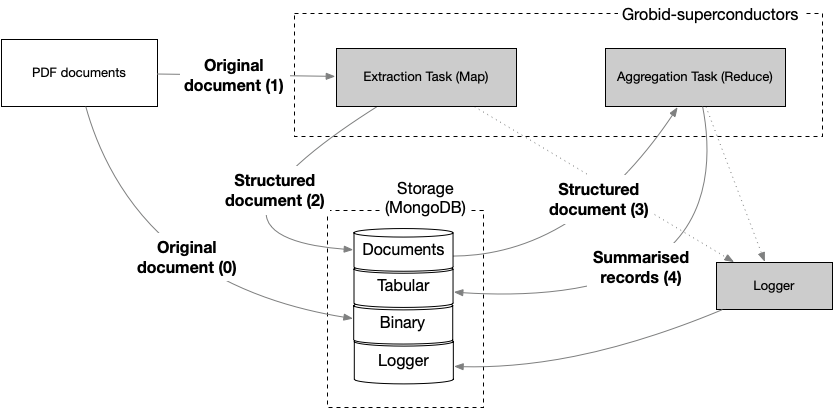
\includegraphics[width=\textwidth]{figures/curation/ingestion-schema.png} 
  \caption{Ingestion process}
  \label{fig:map-reduce}
\end{figure}

Storage is implemented using MongoDB~\footnote{\url{https://www.mongodb.com}}, an open source document database, and the collections are designed as different stages in the processing: 
\begin{itemize}
    \item the \textbf{binary} collection contains the original PDF documents 
    \item the \textbf{documents} collection contains the structured document
    \item \textbf{tabular} collection stores the summarised records, and finally 
    \item \textbf{logger} contains detailed information on the status of the process of each document, including eventual errors information. More details are given in Section~\ref{subsec:curation-and-processing-logs}.
    \item \textbf{training\_data} Used to collect training examples in and discussed in Section~\ref{subsec:feedback-loop-training-data}.
\end{itemize}


The "Extraction Task" takes the PDF documents in input and transforms them into a rich representation document that includes text passages (sentences, paragraphs), annotations, and tokens as JSON files, which we will refer to as \textit{structured documents} (Figure~\ref{fig:data-flow-2}). 

\begin{figure}[htbp]
  \centering
  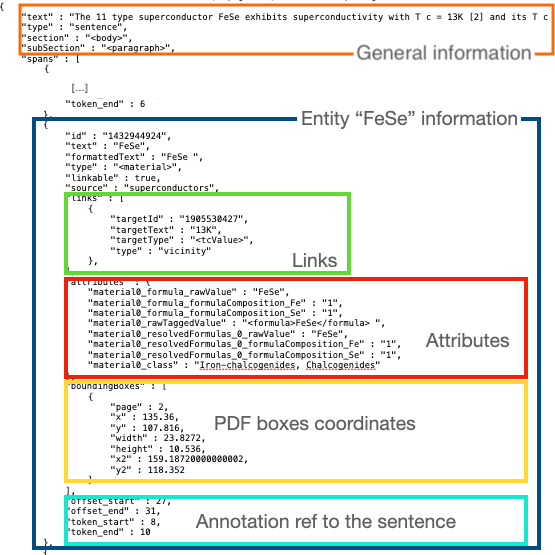
\includegraphics[width=0.8\textwidth]{figures/curation/data-flow-2} 
  \caption{Example of the information from one single entity from a passage extracted in the "Extraction Task". The different structured information are highlighted: links, attributes, PDF boxes coordinates (to visualise annotations on the PDF document), and annotations references within the passage (to visualise annotations on text).}
  \label{fig:data-flow-2}
\end{figure}

Each passage is composed of the following attributes: the text of the passage, the type (whether it is a sentence or paragraph), the main section: header, body, and annex, and the subsections: title, abstract, paragraph, caption.
Furthermore, a passage also contains the list of spans representing the extracted entities and a list of layout tokens. 
The spans are characterised by text, type, attributes, a unique identifier, and other internal information (e.g. from which ML model the entity was extracted). 
The attributes are stored as a key-value and mainly contain information extracted by the material parser such as, for example, the chemical formula, the structured composition, the material class, and so on.
The layout tokens contain low-level information coming from the PDF document: font size, font face, superscript, subscript, bold, italic, and coordinates within the PDF document. The coordinates are a couple of x,y numbers that are used to build annotation "boxes" to encapsulate each token independently (see Figure~\ref{fig:pdf-view} in the following chapter, as an example). 

The "Aggregation Task" takes the structured document as input and reduces it to a table format where each row (referred to as a \textit{summarised record}, or, simply \textit{record}) pivots around the relation materials-Tc and attaches additional elements to it. 
The number of aggregated records can increase when large entities are extracted and may contain condensed information referring to multiple materials. 
For example, the raw material "Zn and CU doping La Fe B" will be aggregated as two records (doping: Zn, formula: La Fe B) and (doping: Cu, formula: La Fe B). 

In the following listing, we illustrate an example of aggregated record: lines 2-21 contain the records information such as material name, \tc, pressure, etc. Lines 22-34 represent the list of spans, which are the original annotation information. They are used to link the aggregated records back to the original structure document information. 
Line 35, 'hash' is a unique signature of the original document using the first 10 characters of the MD5 hash function on the binary content. We use this information to link the original document, the structured document, and the summarised records.
'type', 'timestamp' and 'status' are internal workflow information, discussed in the next chapter. 
The rest of the lines contains the bibliographic data (39-42).

\begin{lstlisting}[numbers=left,numbersep=5pt,caption=Example of record related to the FeSe material after the aggregation.]
{
  "_id": ObjectId("63dcae91e4d716dd10dd5a7d"),
  "rawMaterial": "FeSe",
  "materialId": "1432944924",
  "name": null,
  "formula": "FeSe",
  "doping": null,
  "shape": null,
  "materialClass": "Chalcogenides, Iron-chalcogenides",
  "fabrication": null,
  "substrate": null,
  "variables": null,
  "criticalTemperature": "13K",
  "criticalTemperatureId": "1905530427",
  "measurementMethod": "",
  "measurementMethodId": "",
  "appliedPressure": null,
  "appliedPressureId": null,
  "section": "body",
  "subsection": "paragraph",
  "sentence": "The 11 type superconductor FeSe exhibits superconductivity with T c = 13K [2] and its T c reaches 37K under high pressure (4-6 GPa) [3,4].",
  "spans": [
    {
      "id": "1432944924",
      "text": "FeSe",
      "type": "<material>",
      "linkable": false,
      "offset_start": 27,
      "offset_end": 31,
      "token_start": 0,
      "token_end": 0
    },
    [...]
  ],
  "hash": "f70a71214f",
  "type": "automatic",
  "timestamp": ISODate("2022-11-24T09:02:53.256Z"),
  "status": "new",
  "title": "Evidence of Inhomogeneous Superconductivity in FeTe1-xSexby Scotch-Tape Method",
  "doi": "10.1143/jpsj.81.113707",
  "authors": "Hiroyuki Okazaki, Tohru Watanabe, Takahide Yamaguchi, Yasuna Kawasaki, Keita Deguchi, Satoshi Demura, Toshinori Ozaki, Saleem. J. Denholme, Yoshikazu Mizuguchi, Hiroyuki Takeya, Yoshihiko Takano",
  "publisher": "Physical Society of Japan",
  "journal": "Journal of the Physical Society of Japan",
  "year": 2012
}
\end{lstlisting}





\section{Results}
\label{sec:results-supercon2}

SuperCon\textsuperscript{2} represents the result of our effort to build an automatic TDM process to automatically extract experimental data. 

Compared to the original SuperCon, SuperCon\textsuperscript{2} was collected in a few days. There is no information about how SuperCon was constructed, only that it started in 1987~\cite{ishii2023structuring}. 
When we built the new process to obtain SuperCon\textsuperscript{2}, we were asked to consider two information: ``applied pressure'' and ``measurement method''. 
``Applied pressure'' is the pressure applied to make the material a superconductor and has gained attention because it can radically change the physical structure of a material. Still, at the time of writing, there have been studies that consider this property for material informatics. 
On the other hand, ``measurement method'' is the way scientists measured the superconducting transition temperature \tc and can be used to semantically recognise multiple \tc obtained from the same material or sample. In particular, the identification of calculated properties is fundamental when providing data for predictions. 
These properties were present only for a minority of records in SuperCon and, we hypothesise, that they were not considered in the initial design. The fact that applied pressure was recorded in different fields of the database suggests that such action was more a decision of the curator than a methodological change.
The resulting SuperCon\textsuperscript{2} counted 2052 triplets with applied pressure (\textit{material-\tc-pressure}), and 3602 records with an explicit measurement method (\textit{material-\tc-measurement method}).
The SuperCon\textsuperscript{2} schema is discussed in~\ref{sec:results-supercon2} with examples in Table~\ref{tab:supercon2-schema}. 

However, our TDM process is limited to text, whereas the manual process has also been focussing on plots and tables. This limitation reduces the density of the data that is collected, as observed by the amount of information (33,000 records) extracted from only 7227 articles. Such additions should be built as separate projects.
However, the automatic process cannot be used without manual validation given the high-quality constraints of SuperCon. This gives the opportunity to combine the TDM process with data curation in a homogeneous flow that is described in Chapter~\ref{cha:curation}.

\begin{table}[htpb]
    \centering\small
    \begin{tabular}{lcc}
        \toprule
        \textbf{Category} & \textbf{SuperCon} & \textbf{SuperCon\textsuperscript{2}} \\
        \midrule
        Size (records) & $\sim$33000 & 40324 \\
        Size (papers) & 7227 & 37700 \\
        \# records with applied pressure & 6 & 2052 \\
        \# records with measurement method & 600 & 3602 \\
        Process & Manual & Automatic \\
        Time for process & N/A & A few days \\
        Scope & Text, plots, tables & Text \\
        \bottomrule
    \end{tabular}
    \caption{Comparison in volumes from Supercon and SuperCon\textsuperscript{2}.}
    \label{tab:comparisong-supercon-supercon2}
\end{table}



\afterpage {
    \clearpage % Flush earlier floats (otherwise order might not be correct)
    
    \begin{table}[ht]
        \centering\small
        \caption{Summary and description of the SuperCon\textsuperscript{2} schema. ``Internal information'' is technical information not accessible to the users.}
        \scalebox{0.8}{
            \begin{tblr}{Q[l,m]Q[r,m]Q[r,m]}
                \hline[1pt]
                \textbf{Field name} & \textbf{Description}                             & \textbf{Examples}             \\
                \hline
                \SetCell[c=3]{c}{\emph{Material information}}                                                        \\
                \hline[dashed]
                {Raw                                                                                                   \\ material} & The material or sample as it appears in the text &\\
                \hline[dotted]
                Name                & Canonical name of a material                     & {PCCO, PCO, Metal diboride,   \\ hydrogen, carbon} \\
                \hline[dotted]
                Formula             & {Material expressed as chemical formula. This                                    \\ includes also formulas with stochiometric variables} & {$Pr_{1.869}Ce_{0.131}CuO_4-\delta$,\\ $MgB_2$, $La_{2-x} Sr_x CuO_4$} \\
                \hline[dotted]
                Doping              & {Doping ratio and doping materials                                               \\ that might be adjoined to the material} & {Overdoped, underdopded,\\ optimally doped,\\ bulk, pure, 1\% Zn, Zn\\ (from Zn-doped XYZ)}\\
                \hline[dotted]
                Shape               & The shape of the material or the sample          & {Single crystal, polycrystal, \\ wire, powder, film} \\
                \hline[dotted]
                Variables           & Variables that can be substituted in the formula & x = 0, RE=Ln,St               \\
                \hline[dotted]
                Class               & {Material classification according                                               \\ to the domain-experts taxonomy} & cuprates, oxides, and alloys\\
                \hline[dotted]
                Fabrication         & {All the information that does not                                               \\ belong to any of the previous tags} &  {Intercalated,\\ synthesized by MBE method,\\ electron-doped, hole-doped} \\
                \hline[dotted]
                Substrate           & Substrate material described in the raw material & {PCCO films onto              \\ $Pr_2 CuO_4 (PCO)/SrTiO_3$ }\\
                \hline[dashed]
                \SetCell[c=3]{c}{\emph{Properties}}                                                                  \\
                \hline[dashed]
                {Critical                                                                                              \\ Temperature}  & Superconducting critical temperature &\\
                \hline[dotted]
                {Applied                                                                                               \\ Pressure}  & {Pressure applied when measuring \\ the superconducting critical temperature} &\\
                \hline[dotted]
                {Measurement                                                                                           \\ Method}  & {Method for measurement of the\\ superconducting critical temperature} & {Magnetic susceptibility,\\ specific heat, calculation,\\ prediction, resistivity}\\
                \hline[dashed]
                \SetCell[c=3]{c}{\emph{Document bibliographic information}}                                          \\
                \hline[dashed]
                Section             & The main body section of the paper               & Header, body, annex           \\
                \hline[dotted]
                Subsection          & The secondary segmentation area of the paper     & {Paragraph, table caption,    \\ figure caption, title, abstract} \\
                \hline[dotted]
                {Authors,                                                                                              \\ Title, DOI,\\ Publisher,\\ Journal, Year} & \SetCell[c=2]{c}{Bibliographic information of the document}\\
                \hline[dashed]
                \SetCell[c=3]{c}{\emph{Internal information}}                                                        \\
                \hline[dashed]
                {Hash,                                                                                                 \\ Timestamp} & \SetCell[c=2]{c}{Hash calculated on the binary content of the original PDF\\ document and the timestamp when the document was processed.}\\
                \hline[1pt]
            \end{tblr}
        }
        
        \label{tab:supercon2-schema}
    \end{table}
    \clearpage
}




\section{Conclusions}

This contribution represents the main contribution of this dissertation where our efforts are applied in collecting SuperCon\textsuperscript{2}, which is a database with 40324 records of superconductors materials and properties, including the applied pressure and the \tc~measurement method.
SuperCon\textsuperscript{2}. 
This database is available in various formats at \url{https://github.com/lfoppiano/supercon}.

SuperCon\textsuperscript{2} should not be considered as a replacement of SuperCon but as a staging are where automatically extracted data is collected. Domain-experts can access this data, correct it and push it to SuperCon. 
This approach will reduce the amoutn of human labor required and improve the overall quality of the data, as we demosntrate in the next Chapter~\ref{cha:curation}.

\chapter{Techniques for mitigating the impact of manual curation}
\label{cha:curation}
\section{Introduction}

The SuperCon database was built manually from 1987~\cite{ishii2023structuring} by the National Institute for Materials Science (NIMS) in Japan and it is considered a reliable source of experimental data on superconductors~\cite{roter2020predicting, stanev2017machine, tran2022machine, konno2021deep}. 
However, the updates of SuperCon have become increasingly challenging due to the high publication rate. 
In response to the need for a more efficient approach to sustain productivity, we embarked on the development of an automated system for extracting material and property information from the text contained in relevant scientific publications. 
This automated process enabled the rapid creation of ``SuperCon\textsuperscript{2} Database'', a comprehensive database of superconductors containing around 40000 entries, within an operational duration of just a few days (Chapter~\ref{cha:supercon2}). 
Matching the level of quality seen in SuperCon while simultaneously automating the extraction of organised data can be achieved with a properly designed curation process. 
We use the term \emph{curation} to describe the overall process of reviewing and validating database records, while \emph{correction} refers to the specific action of altering the values of one or more properties within an individual record.
At the moment of writing this article, we are not aware of any other curation tool focusing on structured databases of extracted information. 
There are several tools for data annotation, such as Inception~\cite{klie-etal-2018-inception}, and Doccano~\cite{doccano} which concentrate on text labelling and classification.

In this contribution, we designed and developed a workflow with a user interface, ``SuperCon\textsuperscript{2} Interface'', crafted to produce structured data of superior quality and efficiency to the one obtained by the ``traditional'' manual approach consisting of reading documents and noting records, usually on an Excel file.
We developed this framework around the specific use case of SuperCon, however, our goal is to be adapted to alternative data frameworks.

Our contributions can be summarised as follows:
\begin{itemize}
    \item We developed a workflow and a user interface that allow the curation of a machine-collected database. We demonstrate that using it for data correction resulted in higher quality than the ``traditional'' (manual) approach.
    \item We devise an anomaly detection process for incoming data lower rejection rate (false positive rate) from domain experts.
    \item We propose a mechanism that selects training data based on corrected records, and we demonstrate that such selections are rapidly improving the ML models.
\end{itemize}

\section{Curation workflow}
\label{sec:curation-workflow}
The curation of the SuperCon\textsuperscript{2} Database acts as a workflow where user actions result in database records state transitions (Figure~\ref{fig:curation-workflow}). 
Allowed manual actions include a) \textit{mark as valid} (validation) when a record is considered correct or corrected by someone else. When a record is not valid, users can: b) \textit{mark as invalid} when considered ``potentially'' invalid (or the curator is not confident), c) perform \textit{manual correction} to update it according to the information from the original PDF document, and d) \textit{remove} the record when it was not supposed to be extracted.

In addition to manual operations by users, this workflow also supports automatic actions: ``anomaly detection'' for prescreening records (Section~\ref{subsec:anomaly-detection}) and the ``training data collector'' for accumulating training data to improve ML models (Section~\ref{subsec:feedback-loop-training-data}). 


Although only the most recent version of a record can be viewed in this system, the correction history is recorded (Section~\ref{subsec:curation-and-processing-logs}). 


\begin{figure}[htbp]
  \centering
  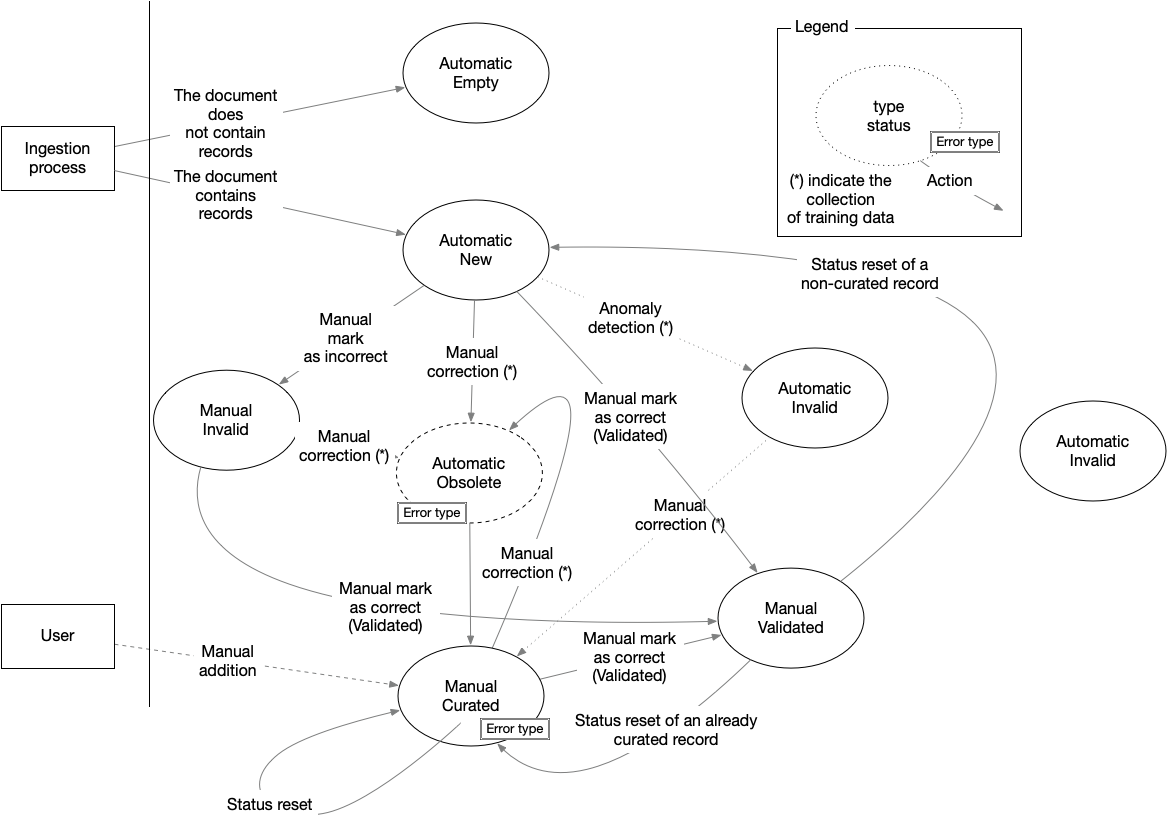
\includegraphics[width=1\textwidth]{figures/curation/record-correction} 
  \caption{Schema of the curation workflow. Each node has two properties: type and status (Section~\ref{subsec:curation-status}). Each edge indicates one action. The workflow starts on the left side of the figure. The new records begin with ``Automatic, New''. Changes of state are triggered by automatic (Section~\ref{subsec:anomaly-detection}) or manual operations (update, mark as valid, etc.. Section~\ref{subsec:manual_correction}) and results in changes of the properties in the node. Each combination of property values identifies each state. ``(*)'' indicates a transition for which the training data are collected (Section~\ref{subsec:feedback-loop-training-data})}
  \label{fig:curation-workflow}
\end{figure}


\subsection{Workflow control}
\label{subsec:workflow-control}
The workflow state is determined by the ``curation status'' (Section~\ref{subsec:curation-status}), the user action, and the error type (Section~\ref{subsec:error-types}).

\subsubsection{Curation status} 
\label{subsec:curation-status}
The curation status (Figure~\ref{fig:curation-workflow}) is defined by \emph{type} of action, manual or automatic, and \emph{status}, which can assume the following values: 
\begin{itemize}
    \item \textbf{new}: default status when a new record is created.
    \item \textbf{curated}: the record has been amended manually.
    \item \textbf{validated}: the record was manually marked as valid.
    \item \textbf{invalid}: the record is wrong or inappropriate for the situation (e.g., T\textsubscript{m} or T\textsubscript{curie} extracted as superconducting critical temperature).
    \item \textbf{obsolete}: the record has been updated and the updated values are stored in a new record (internal status\footnote{``internal status'' indicates that their records should be hidden in the interface}).
    \item \textbf{removed}: the record has been removed by a curator (internal status).
\end{itemize} 
    

\subsubsection{Error types}
\label{subsec:error-types}
We first introduced \emph{error type} in~\cite{foppiano2023automatic} and extended their scope in this work to consider data curation and anomaly detection. 

Users are required to select one \emph{Error Type} at every record update or removal. This information is stored in the ``original'' record and can be different at every record modification.
The error type values can be summarised as follows: 

\begin{itemize}
    \item \textbf{From table}: the entities Material $\rightarrow$ T\textsubscript{c} $\rightarrow$ Pressure are identified in a table. At the moment, table extraction is not performed
    \item \textbf{Extraction}: The material, temperature, and pressure are not extracted (no box) or extracted incorrectly. 
    \item \textbf{Linking}: The material is incorrectly linked to the T\textsubscript{c} given that the entities are correctly recognised.
    \item \textbf{T\textsubscript{c} classification}: The temperature is not correctly classified as ``superconductors critical temperature'' (e.g., Curie temperature, Magnetic temperature...).
    \item \textbf{Composition resolution}: The exact composition cannot be resolved (e.g., the stoichiometric values cannot be resolved).
    \item \textbf{Value resolution}: The extracted formula contains variables that cannot be resolved, even after having read the paper. This includes when data is from tables
    \item \textbf{Anomaly detection}: The data has been modified by anomaly detection, which facilitates their retrieval from the interface.
    \item \textbf{Curation amends}: The curator is updating the data which does not present issues due to the automatic system.
\end{itemize}

\subsection{Anomaly detection}
\label{subsec:anomaly-detection}
Anomaly detection is the process of identifying unusual events or patterns in the data. 
In our context, this means identifying data that are greatly different from the expected values.
This post-process was introduced in a limited scope to draw attention to certain cases during the curation.

The anomaly detection uses a rule-based approach and marks any record that matches the following conditions
\begin{itemize}
    \item the extracted T\textsubscript{c} is greater than room temperature (273 K), negative, or contains invalid characters and cannot be parsed (e.g. ``41]'')
    \item the chemical formula cannot be processed by an ensemble composition parser that combines Pymatgen~\cite{Ong2013}, and text2chem~\cite{kononova2019text} 
    \item the extracted applied pressure cannot be parsed or falls outside the range 0 - 250 GPa.
\end{itemize}

Records identified as anomalies have \emph{status} ``invalid'' and \emph{error type} ``anomaly detection'' for easy identification.
Since this process may find false positives, its output requires validation from curators. 
For example, in certain contexts, T\textsubscript{c} values above room temperature or applied pressure up to 500 GPa may be valid in researchers' hypotheses, calculations or simulated predictions. 

We ran the anomaly detection on the full SuperCon\textsuperscript{2} Database (40324 records~\cite{foppiano2023automatic}). 
The anomaly detection identified 1506 records with invalid T\textsubscript{c}, 5021 records with an incomplete chemical formula, 304 records with invalid applied pressure, and 1440 materials linked to multiple T\textsubscript{c} values. 
Further analysis and cross-references with contrasting information may be added in future. 

\subsection{Automatic training data collector}
\label{subsec:feedback-loop-training-data}
The curation process is a valuable endeavour demanding significant knowledge and human effort. 
To maximise the use of this time for collecting as much information as possible.
We integrated an automatic procedure in the curation process that, for every correction, accumulates the related data examples that can be used to improve the underlying ML models. 

\subsubsection{Training data collection}
In the event of a correction (update, removal) in a database record, this process retrieves the corresponding raw data: the text passage, the recognised entities (spans), and the layout tokens information. 
This information is sufficient to be exported as training examples, which can be examined and corrected, and feedback to the ML model. 

In detail, the process performs the following actions:
\begin{itemize}
    \item The updated record is prepared and stored.
    \item The raw data originating the updated record is identified. First, the corresponding structured document is retrieved from the document collection using the document identifier (the hash). Then, the exact text passage in the structured document is located using a unique id assigned to each material in the database records.
    \item If the raw data has already been collected, it is skipped. This is the case when multiple records belonging to the same text passage are corrected.
    \item Otherwise, the raw information comprising the text string, the spans, and the layout tokens are collected and saved in a separate collection.
    \item The data collected is then sufficient to generate workable instances in different output formats and the related feature files.
\end{itemize}

\subsubsection{Training data management}
We designed a specific page of the interface (Section~\ref{sec:user-interface}) to manage the collected data (Figure~\ref{fig:training-data-view}) in which each row corresponds to a training example composed by the decorated text showing the identified entities, the document identifier, and the status. 
The users can examine the data, delete it, send it to the annotation tool to be corrected, and then export them.
We integrated our interface with Label-studio~\cite{Label_Studio} for the correction of the collected training examples. 
Label-studio is an open-source, python-based, and modern interface supporting many different TDM tasks (NER, topic modelling, image recognition, etc.). 

\begin{figure}[htpb]
  \centering
  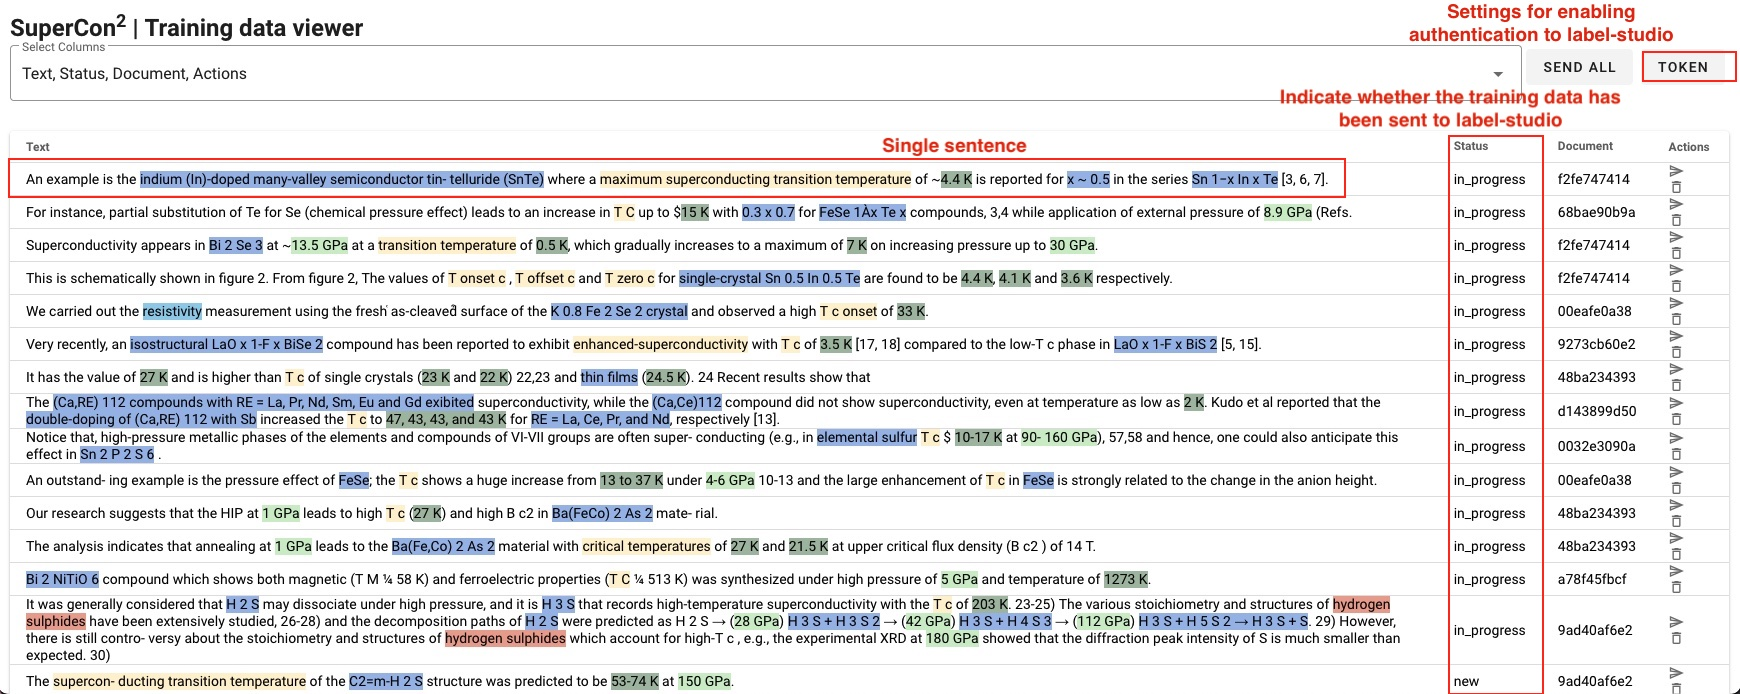
\includegraphics[width=1\textwidth]{figures/curation/training-data-viewer} 
  \caption{Screenshot of the training data management page in the SuperCon\textsuperscript{2} interface. Each row contains one potential training data example. Each example is composed of a sentence and its extracted entities (highlighted in colour) with potential annotation mistakes that need to be corrected using an external tool: we used Label-Studio~\cite{Label_Studio}. The column ``Status'' indicate whether the example has been sent or not to the external tool.}
  \label{fig:training-data-view}
\end{figure}

\section{Curation interface}
\label{sec:user-interface}

The workflow is operated through the user interface, which offers several key features to facilitate the data curation process (Figure~\ref{fig:curation-workflow}).
It provides a comprehensive view of materials and their related properties as a table that includes search, filter, and sorting functionality (Figure~\ref{fig:curation-interface-database}). 
The detailed schema, including examples, is reported in our previous work~\cite{foppiano2023automatic}.

\begin{figure}[htbp]
  \centering
  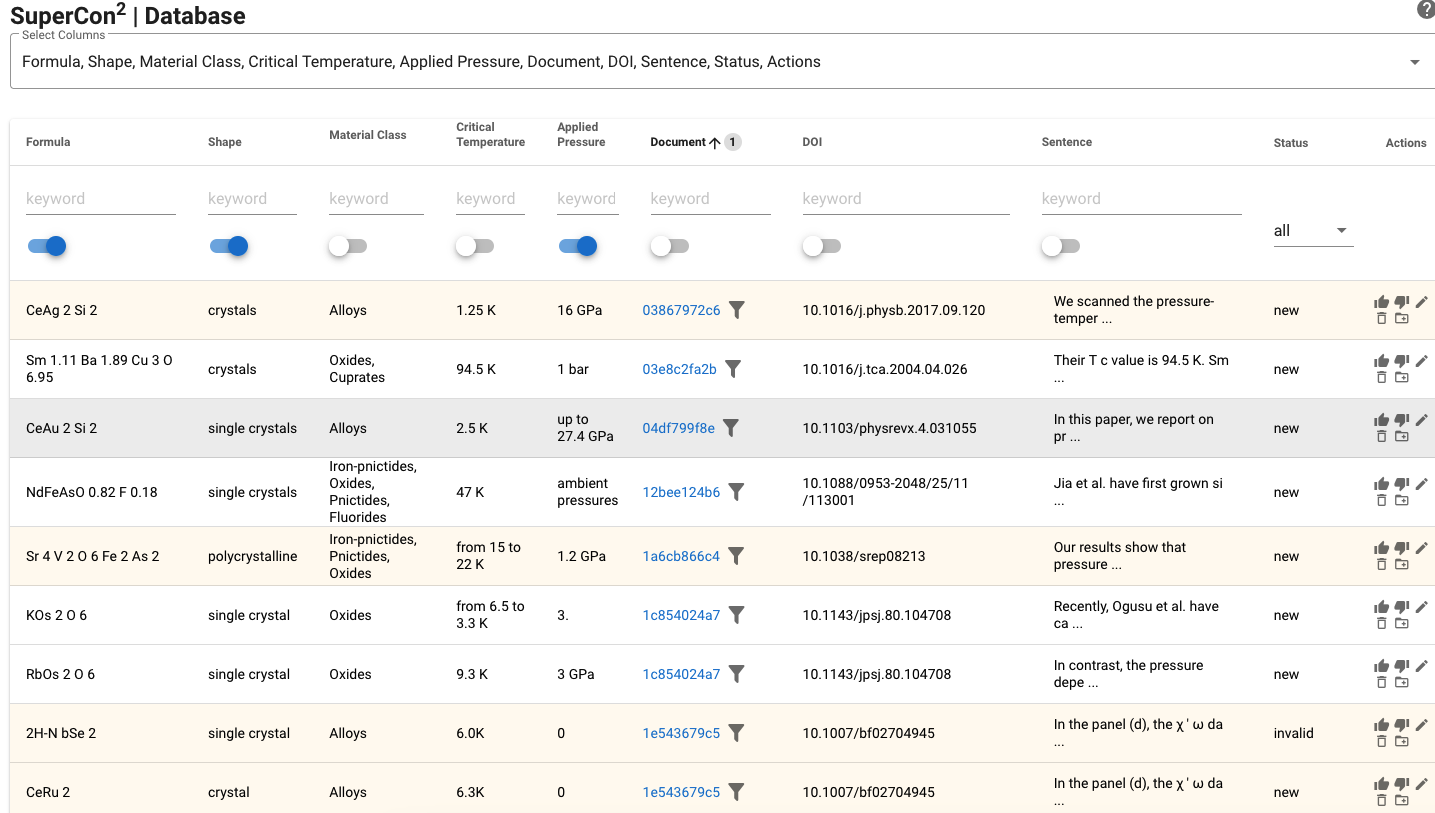
\includegraphics[width=1\textwidth]{figures/curation/supercon-curation-database.png} 
  \caption{Screenshot of SuperCon\textsuperscript{2} interface showing the database. Each row corresponds to one material-T\textsubscript{c} pair. On top, there are searches by attribute, sorting and other filtering operations. On the right (last column) there are curation controls (mark as valid, update, etc.).   Records are grouped by document with alternating light yellow and white. }
  \label{fig:curation-interface-database}
\end{figure}

During the curation process, it is often necessary to switch back and forth between the database record and the related context in the paper (the related paragraph or sentence). 
Our interface provides a viewer for individual documents, which visualises in the same window a table with the extracted records and the original PDF document decorated with annotations that identify the extracted materials and properties (Figure~\ref{fig:pdf-view}). 

\begin{figure}[htbp]
  \centering
  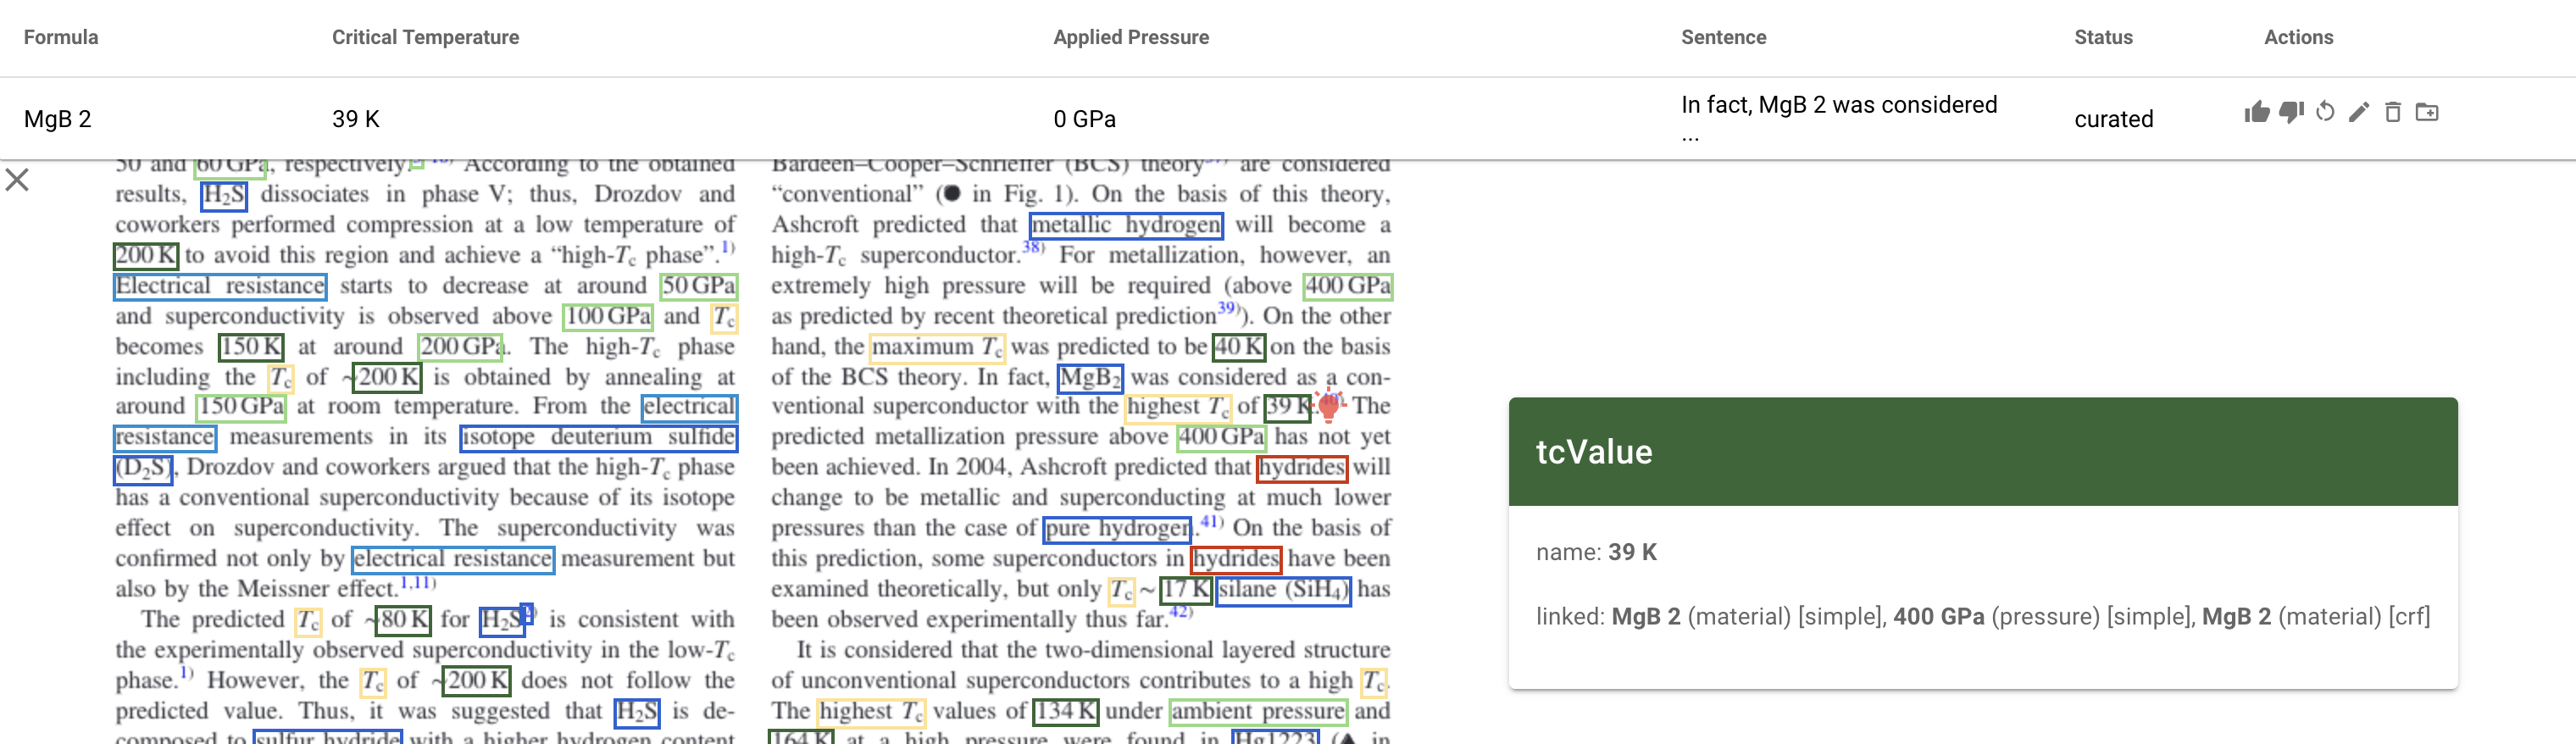
\includegraphics[width=1\textwidth]{figures/curation/pdf-view-context.png} 
  \caption{PDF document viewer showing an annotated document. The table on top is linked through the annotated entities. The user can navigate from the record to the exact point in the PDF, with a pointer (the red bulb light) identifying the context of the entities being examined. }
  \label{fig:pdf-view}
\end{figure}

% Through the interface, users can transition the record through the workflow as previously described . 
% Adding new records is limited to documents already in the database. When a record is added to a document, the record's bibliographic data are copied from other records in the same documents and the user has to only fill up the correct experimental information (material, Tc, etc.).


% The interface automatically collects training data; when a record is amended, the information pertaining it's raw source information (sentence text, annotations) is collected (Section~\ref{subsec:feedback-loop-training-data}). 

% \begin{figure}[htbp]
%   \centering
%   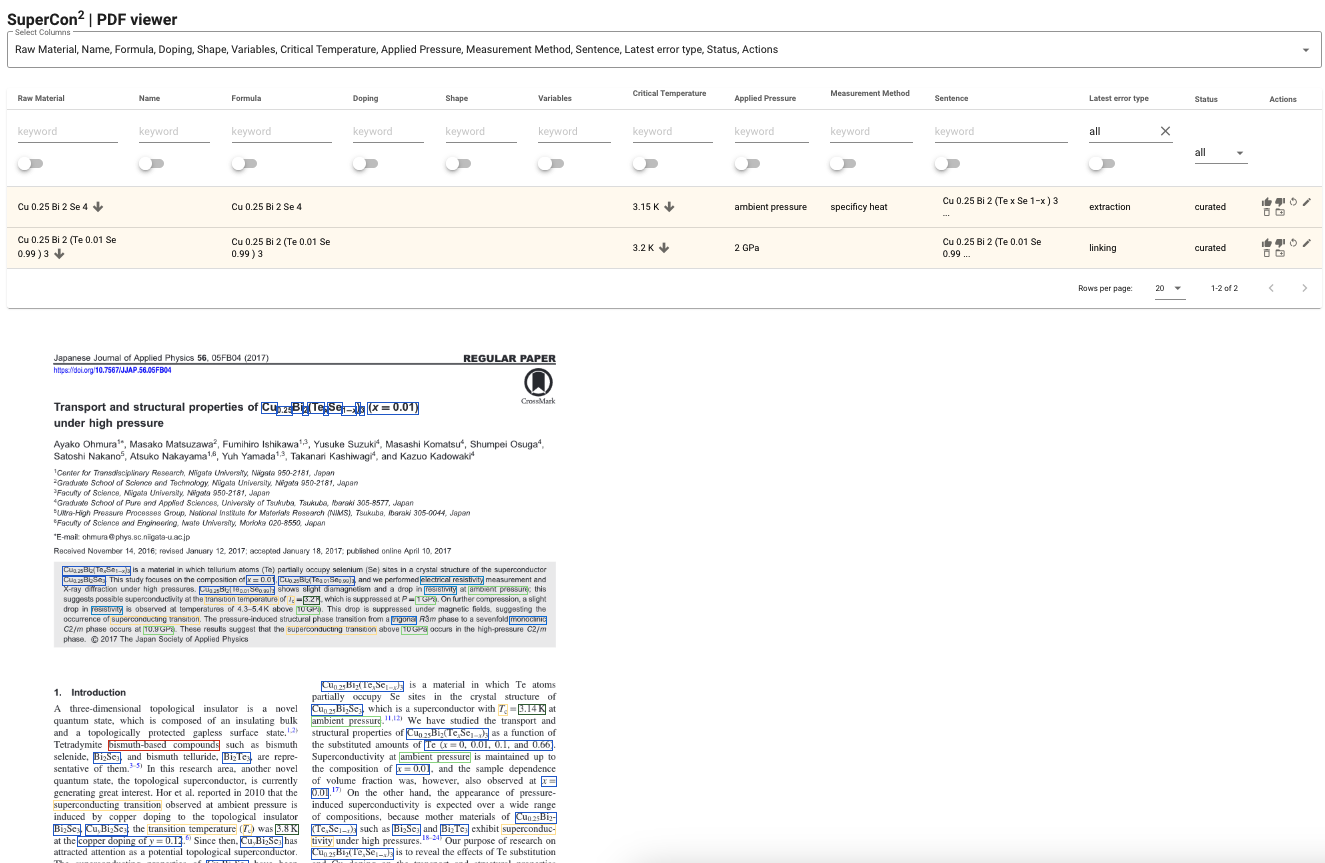
\includegraphics[width=1\textwidth]{figures/curation/supercon-curation-pdf-viewer} 
%   \caption{PDF viewer. The page includes a table showcasing records extracted from the  current document, along with the PDF content and accompanying annotations.}
%   \label{fig:curation-interface-pdf-viewer}
% \end{figure}


\subsection{Manual curation approach}
\label{sec:data-correction}
\label{subsec:manual_correction}

In this section, we discuss our strategy regarding manual curation, which is still indispensable for developing high-quality structures. 
% from automatically may contain incorrect information.
% We have set up an automatic process for anomaly detection (Section~\ref{subsec:anomaly-detection}) which can help to speed up the process but it only detects "potential" problems and requires anyway a manual validation.

We selected curators from domain experts in the field, to certify sufficient data quality. 
Nevertheless, as confirmed from our experiment in Section~\ref{sec:interface-evaluation}, the experience of each individual may have an impact on the final result.
We followed two principles to guarantee robustness in the curation process. 
First, we built solid curation documentation as a form of example-driven guidelines with an iterative approach we first introduced in \cite{foppiano2021supermat}. 
Then, we used a double-round validation approach, in which the data was initially corrected by one person, and validated in a second round, by a different individual. 


\subsection{Curation guidelines}
\label{subsec:curation-guidelines}

The guidelines consist mainly of two parts: the general principles and the correction rules with examples of solutions.
The guidelines are designed to provide general information applied to corrections and very basic explanations containing illustrations for a faster understanding (e.g. the meaning of the colours of the annotations). 
% This helps new curators catch up with the required level of curation precision quickly. 
Differently from our previous work~\cite{foppiano2021supermat}, these guidelines are divided into examples for different scenarios based on the error types mentioned in Section~\ref{subsec:error-types}.
Each example described the initial record, its context, the expected corrected record and a brief explanation, as illustrated in Figure~\ref{fig:example-curation-sheet}. 

\begin{figure}[htbp]
  \centering
  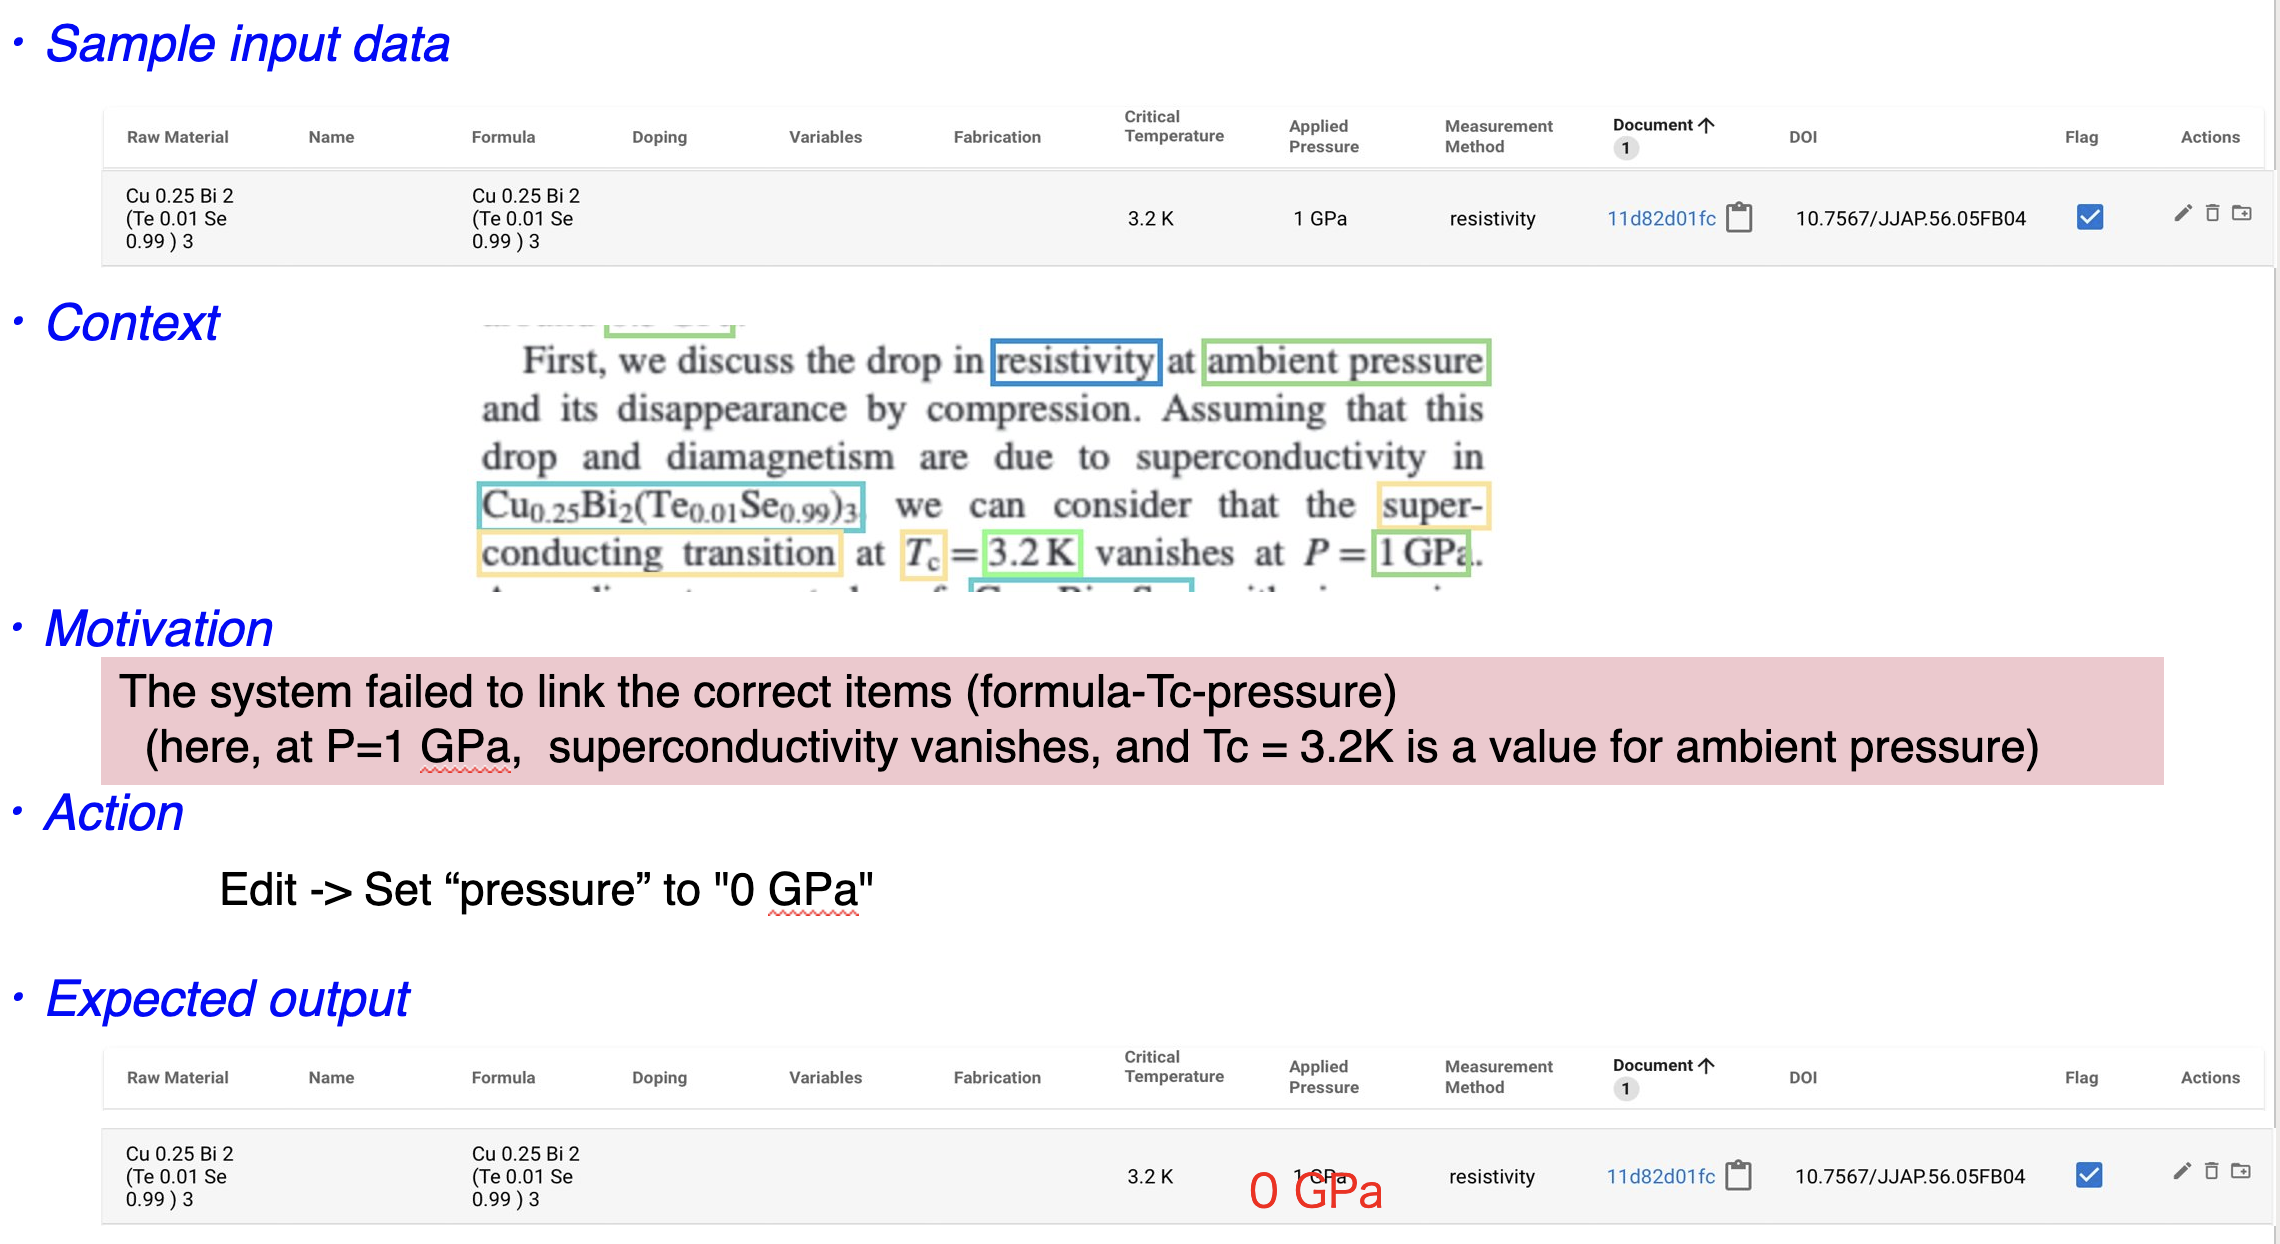
\includegraphics[width=1\textwidth]{figures/curation/example-sheet-curation.png} 
  \caption{Sample curation sheet from the curation guidelines. The sheet is composed of the following information: a) {Sample input data}: a screenshot of the record from the ``SuperCon\textsuperscript{2} Interface'', b) \textit{Context} represented by the related part of the annotated document referring to the record in exams. c) The \textit{Motivation}, describing the issue, d) the \textit{Action} to be taken, and the \textit{Expected output}.
 }
  \label{fig:example-curation-sheet}
\end{figure}


\subsection{Curation and processing logs}
\label{subsec:curation-and-processing-logs}

The Supercon\textsuperscript{2} interface gives access to information regarding the ingestion (processing log) and the curation process (curation log). 
The processing log is filled up when the new data is ingested, it was built to have minimal functions able to explain why certain documents haven't been processed (Figure~\ref{fig:processing-curation-log} top). 
For example, sometimes documents fail because they don't contain any text (image PDF documents) or they are too big (more than 100 pages). 
% Grobid was built focusing on speed and robustness, and contains several fail-safe mechanisms to avoid crashing the system when a document is either too big or does not contains valuable information, for example, does not have any text. 
% Old PDF documents (e.g. before 1990) are likely to have been scanned and contain only images. 
% Examples of too big documents are dissertation theses with more than 100 pages, that might be collected by mistake. 

\begin{figure}[htbp]
  \centering
  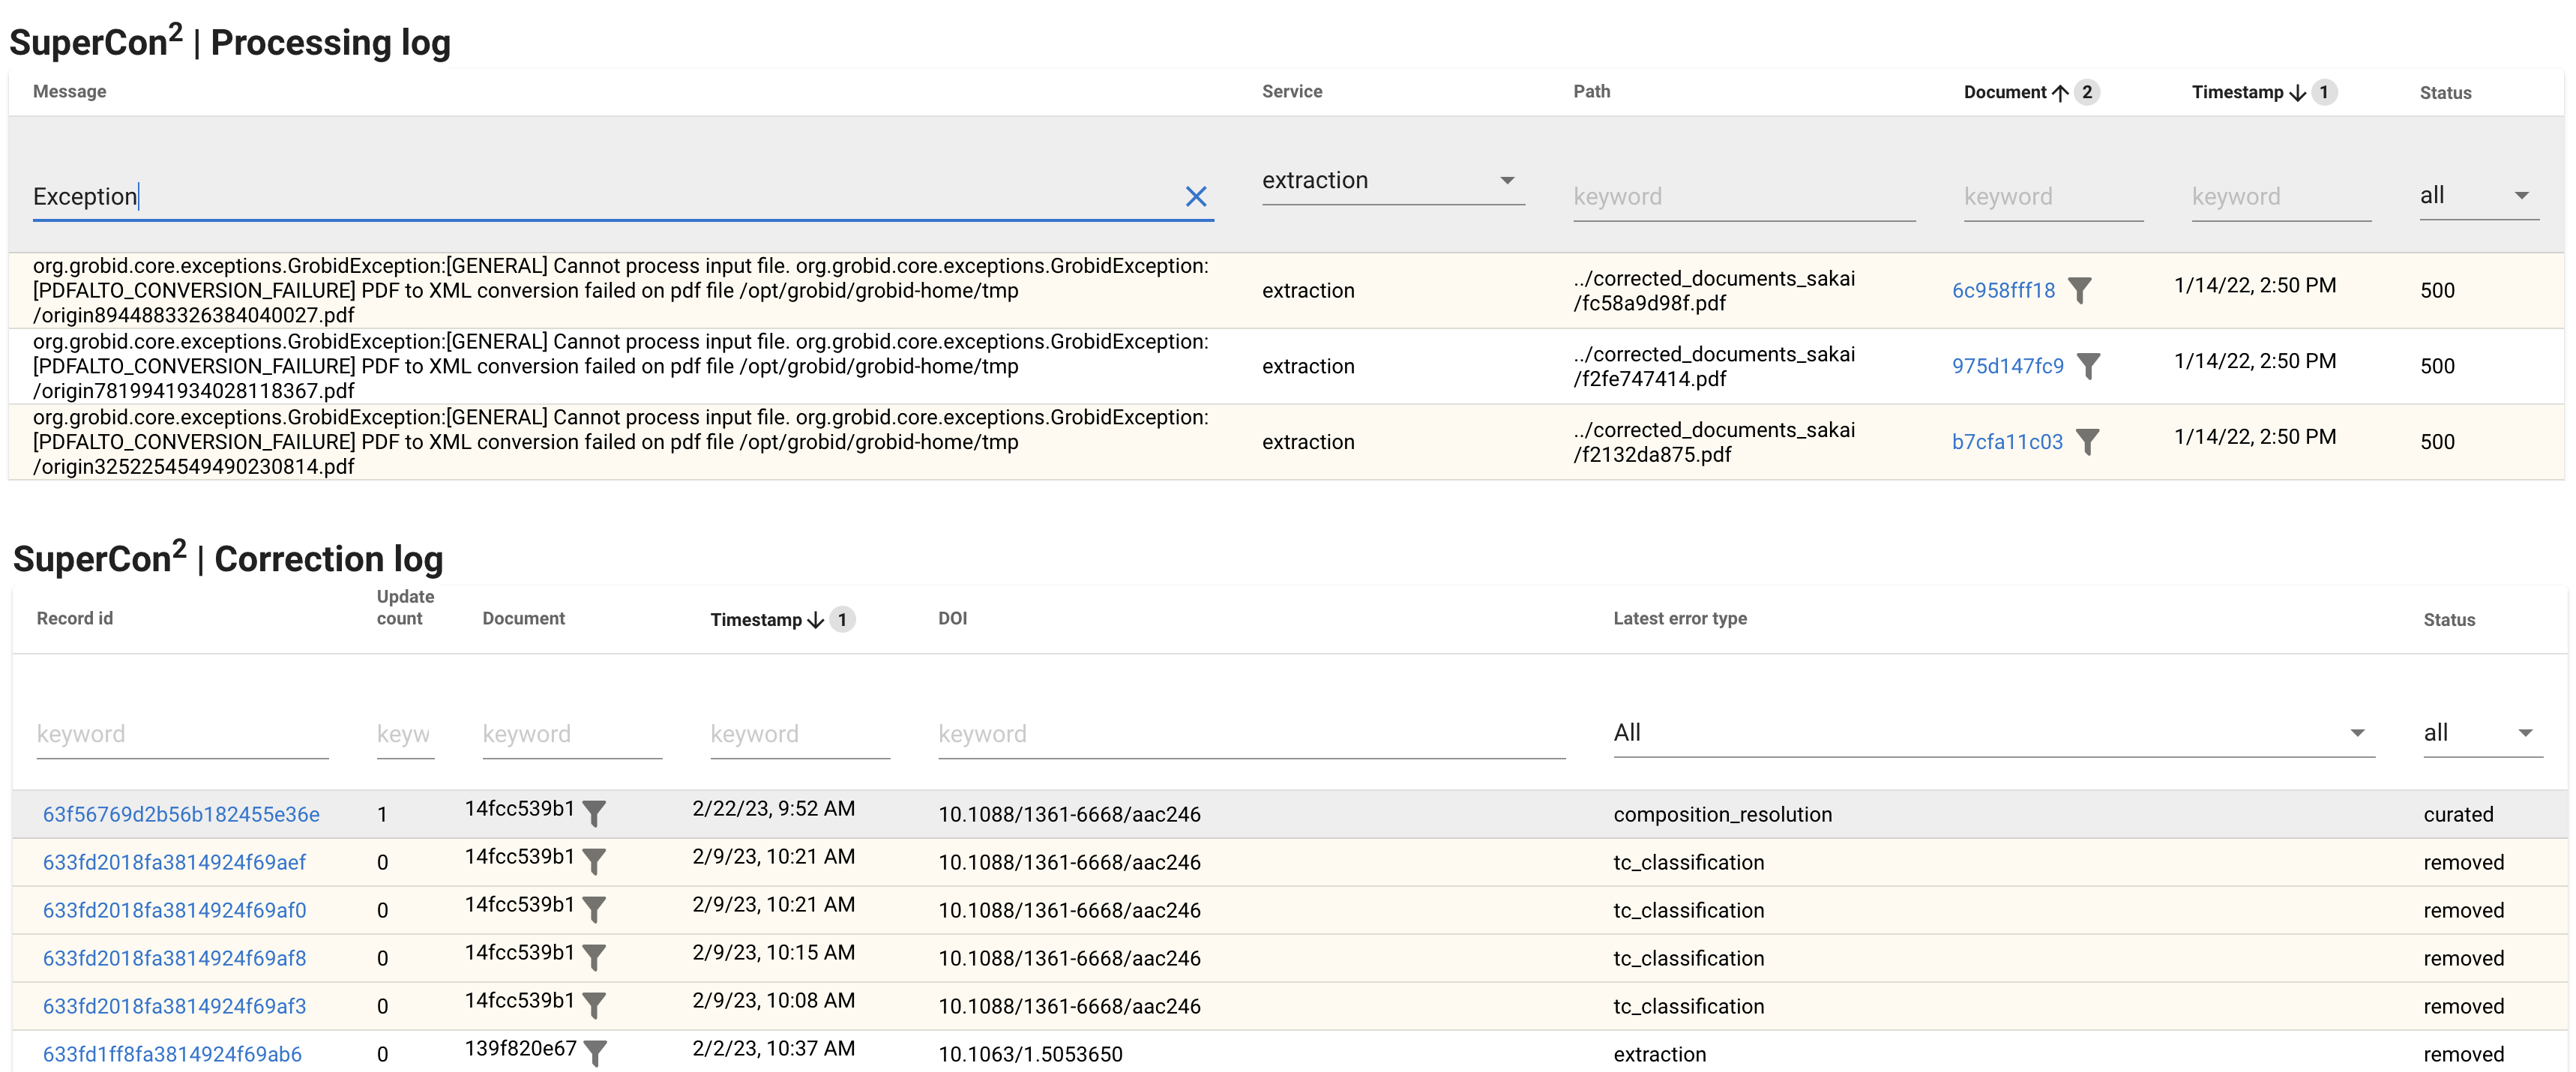
\includegraphics[width=1\textwidth]{figures/curation/processing-curation-log.png} 
  \caption{Top: \textit{Processing log}, showing the output of each ingestion operation and the outcome with the detailed error that may have occurred. Bottom: \textit{Correction log}, indicating each record, the number of updates, and the date/time of the last updates. By clicking on the ``Record id'', is possible to visualise the latest record values.}
  \label{fig:processing-curation-log}
\end{figure}

The curation log provides a view of what, when and how a record has been corrected (Figure~\ref{fig:processing-curation-log} bottom).

% \begin{figure}[htbp]
%   \centering
%   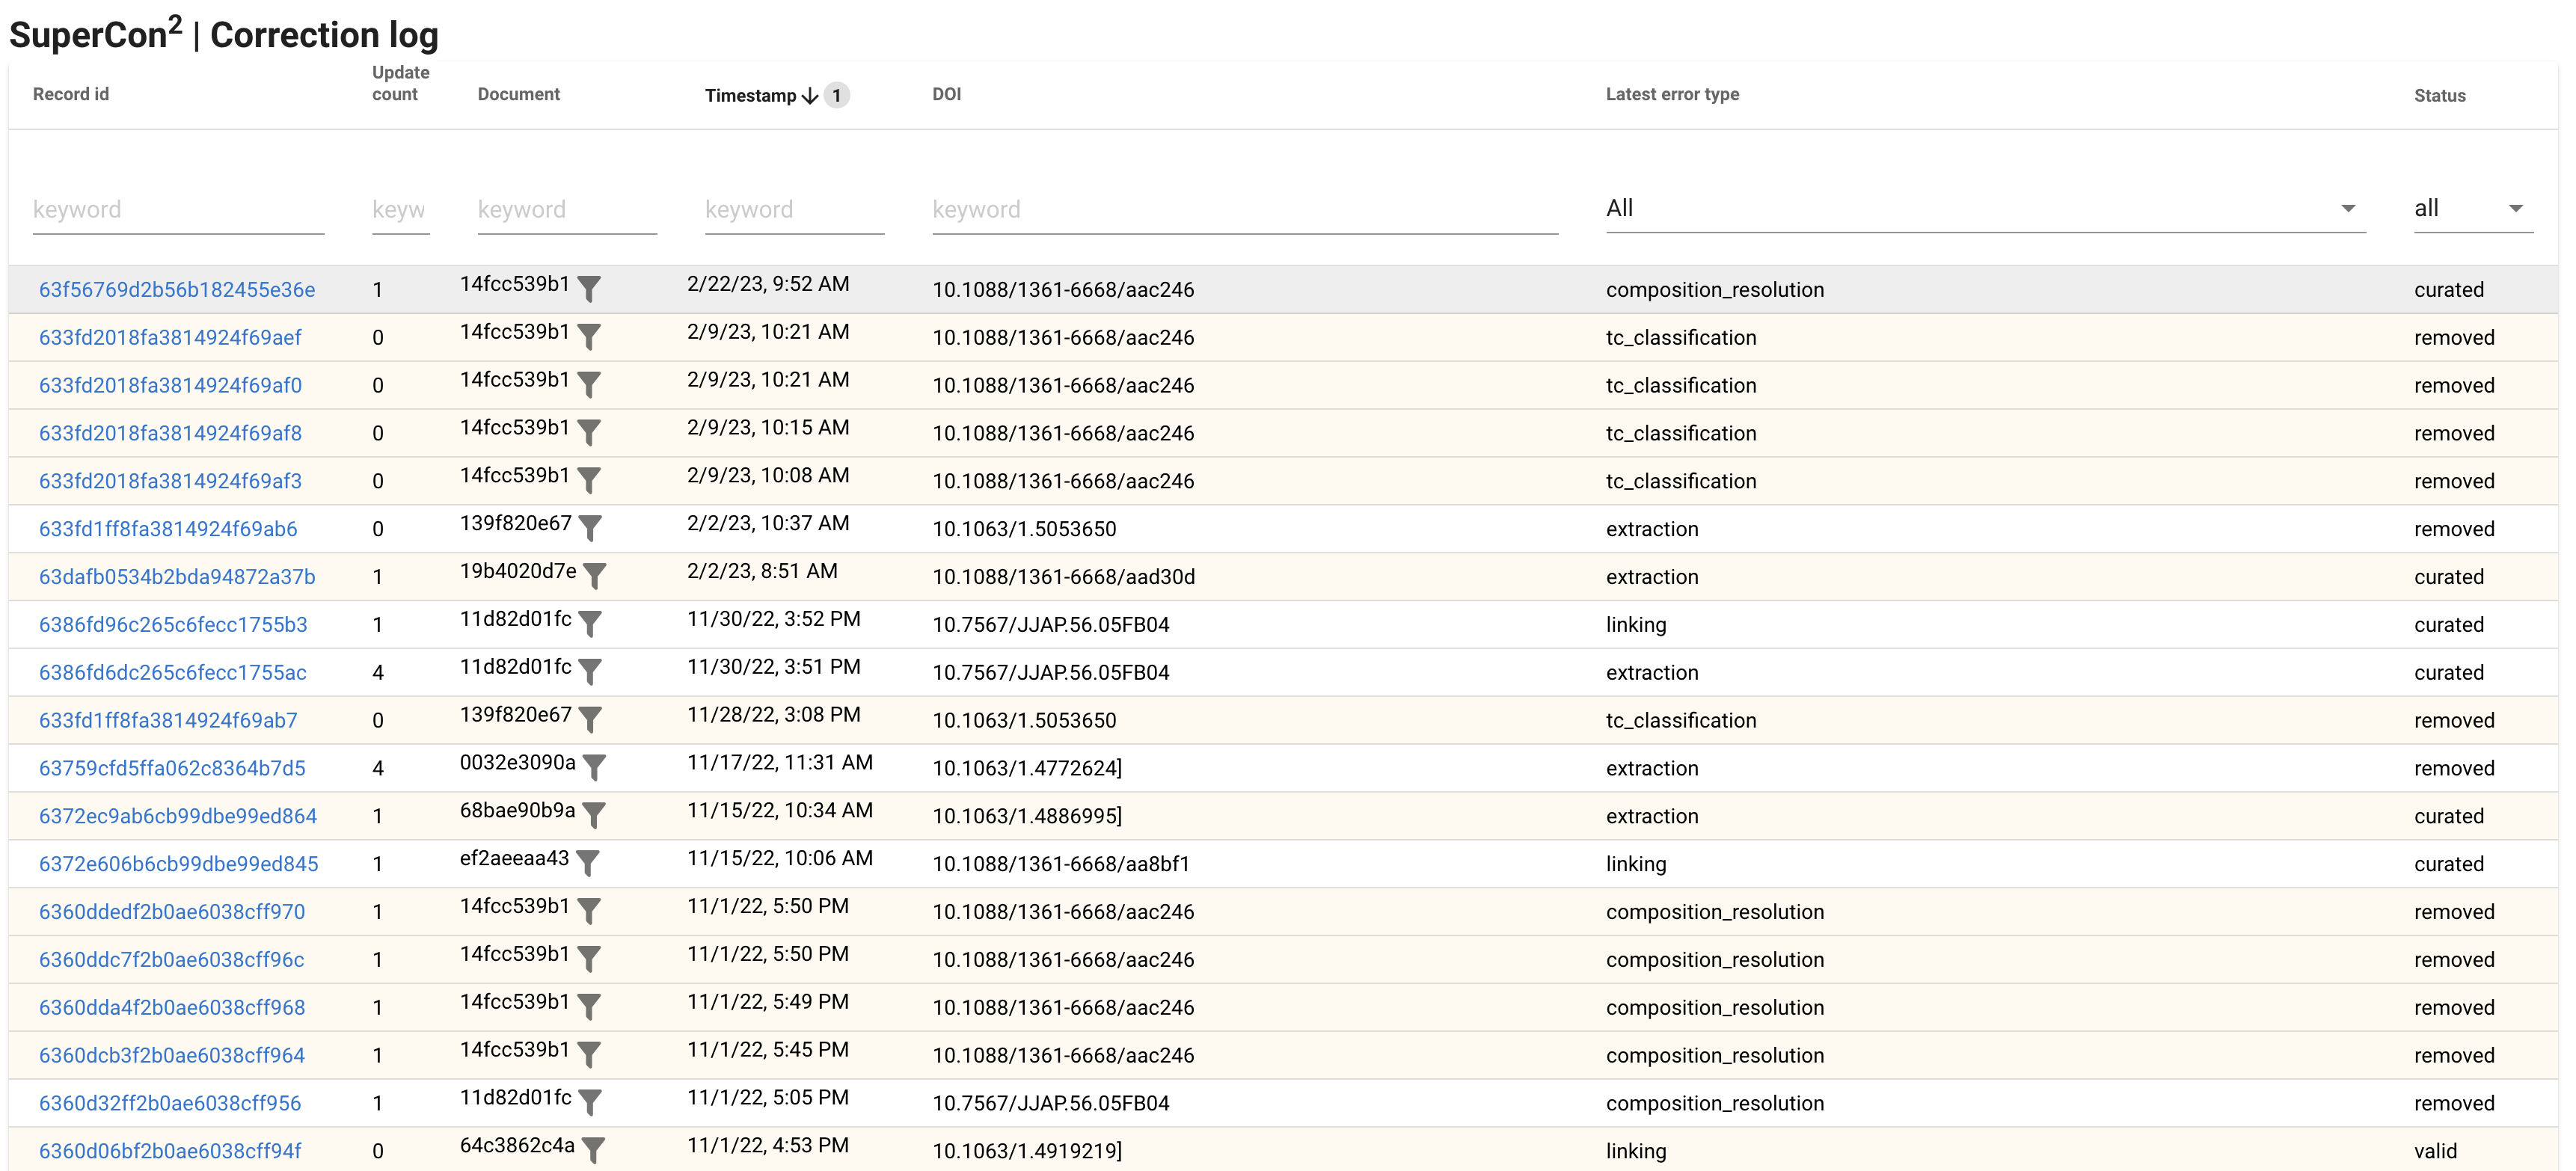
\includegraphics[width=1\textwidth]{figures/curation/curation-log} 
%   \caption{Curation log, indicating each record, the number of updates, and the date/time of the last updates. }
%   \label{fig:curation-log}
% \end{figure}

\section{Results and evaluation}
\label{sec:results-and-evaluation}

In this section, we illustrate the experiments we have run to evaluate our work. 
The evaluation is composed of three sets of results. 
The anomaly detection rejection rate (Section~\ref{subsec:anomaly-detection-evaluation}) indicates how many anomalies were rejected by curators after validation. 
Then, we demonstrate that the training data automatically selected contributed to improving the ML model with a small set of examples (Section~\ref{subsec:training-data-generation-evaluation}) 
Finally, we evaluated the quality of the data extraction using the interface (and the semi-automatic TDM process) against the classical method of reading the PDF articles and noting the experimental information in an Excel file. In Section~\ref{sec:interface-evaluation} we find out that using the interface improves the quality of the curated data by reducing missing experimental data. 


\subsection{Anomaly detection rejection rate}
\label{subsec:anomaly-detection-evaluation}

We evaluated the anomaly detection by observing the ``rejection rate'' which consists of the number of detected anomalies that were rejected by human validation. 
Running the anomaly detection on a database subset with 667 records, it found 17 anomalies in T\textsubscript{c}, 1 anomaly in applied pressure, and 16 anomalies in the chemical formulas. 
Curators examined each reported record and rejected 4 (23\%) anomalies in T\textsubscript{c}, 6 anomalies (37\%) in chemical formulas and 0 anomalies in applied pressure. 
This indicates an appropriate low rate of false positives although a study with a larger dataset might be necessary. 

\subsection{Training data generation}
\label{subsec:training-data-generation-evaluation}
We selected around 400 records in the Supercon\textsuperscript{2} Database that were marked as invalid by the anomaly detection process and we corrected them following the curation guidelines (Section~\ref{subsec:curation-guidelines}).
Then, we examined the corresponding training data corrected by the interface (Section~\ref{subsec:feedback-loop-training-data}) and obtained a set of 352 training data examples for our ML models. 
We call the obtained dataset \emph{curation} to be distinguished from the original SuperMat dataset which is referred to as \emph{base}.

We prepared our experiment using SciBERT~\cite{Beltagy2019SciBERT} that we fine-tuned for our downstream task as in~\cite{foppiano2023automatic}. 
We trained five models that we evaluated using a fixed holdout dataset from SuperMat averaging the results to smooth out the fluctuations. 
We use the DeLFT (Deep Learning For Text)~\cite{DeLFT} library for training, evaluating, and managing the prediction models.  
A model can be trained with two different strategies: 
\begin{enumerate}
    \item \emph{``from scratch''}: when the model is initialised randomly. We denote this strategy with an \emph{(s)}.
    \item \emph{``incremental''}: when the initial model weights are taken from an already existing model. We denote this strategy with an \emph{(i)}.
\end{enumerate}
The latter can be seen as a way to ``continue'' the training from a specific checkpoint.
We thus define three different training protocols: 
\begin{enumerate}
    \item \textbf{base(s)}: using the \emph{base} dataset and training from scratch (s).
    \item \textbf{(base+curation)(s)}: using both the \emph{base} and \emph{curation} datasets and training from scratch (s).
    \item \textbf{base(s)+(base+curation)(i)}: Using the \emph{base} dataset to train from scratch (s), and then continuing the training with the \emph{curation} dataset (i).
\end{enumerate}
We merge ``curation'' with the base dataset because the curation dataset is very small compared to ``base'', and we want to avoid catastrophic forgetting~\cite{overcoming-kirkpatrick-etal-2016} or overfitting.

\begin{table}[htbp]
\centering\small
\caption{F1-score from the evaluation of the fine-tuned SciBERT models. The training is performed with three different approaches. 
The \emph{base} dataset is the original dataset described in~\cite{foppiano2021supermat}, and the \emph{curation} dataset is automatically collected based on the database corrections by the interface and manually corrected. \textit{s} indicate ``training from scratch'', while \textit{i} indicate ``incremental training''. 
The evaluation is performed using the same holdout dataset from SuperMat~\cite{foppiano2021supermat}. 
The results are averaged over 5 runs or train and evaluation. }
\begin{tabular}{lrrr}
\toprule
& \textbf{base(s)} & \textbf{(base+curation)(s)} & \textbf{base(s)+(base+curation)(i)} \\ 
\midrule
Nb total examples & 16902 & 17254 & 16902(s), 17254 (i)\\ 
\midrule
\texttt{<class>}        & 70.41         & \textbf{73.02}         & 71.86 \\ 
\texttt{<material>}     & 79.37         & 80.09         & \textbf{80.37} \\ 
\texttt{<me\_method>}   & 66.72         & 66.57         & \textbf{66.95} \\ 
\texttt{<pressure>}     & 46.43         & \textbf{48.42}         & 47.23 \\ 
\texttt{<tc>}           & 80.13         & \textbf{80.92}         & 80.34 \\ 
\texttt{<tcValue>}      & 78.29         & 78.41         & \textbf{79.73} \\ 
\midrule
\textbf{All (micro avg.)} & 76.67       & 77.44         & \textbf{77.48} \\ 
\midrule
\textbf{$\Delta$ avg. w/ baseline}& -   & +0.77     & \textbf{+0.81} \\ 
\bottomrule
\end{tabular}
\label{tab:evaluation-curation-training2}
\end{table}


The trained models are then tested using a fixed holdout dataset that we designed in our previous work~\cite{foppiano2023automatic} and the evaluation scores are shown in Table~\ref{tab:evaluation-curation-training2}.

This experiment demonstrates that with only 352 examples (2\% of the SuperMat dataset) comprising 1846 additional entities (11\% of the entities from the SuperMat dataset) (Table~\ref{tab:training-support}), we obtain an improvement of F1-score from 76.67\%\footnote{In our previous work~\cite{foppiano2023automatic} we reported 77.03\% F1-score. 
There is a slight decrease in absolute scores between DeLFT 0.2.8 and DeLFT 0.3.0. 
One cause may be the use of different hyperparameters in version 0.3.0 such as batch size and learning rate.
However, the most probable cause could be the impact of using the Huggingface tokenizers library which is suffering from quality issues \url{https://github.com/kermitt2/delft/issues/150}.} to values between 77.44\% (+0.77) and 77.48\% (+0.81) for (base+curation)(s) and base(s)+(base+curation)(i), respectively. 


\begin{table}[htbp]
\centering
\small
\caption{Data support, the number of entities for each label in each of the datasets used for evaluating the ML models. The \emph{base} dataset is the original dataset described in~\cite{foppiano2021supermat}, and the \emph{curation} dataset is automatically collected based on the database corrections by the interface and manually corrected.}
\begin{tabular}{lccc}
\toprule
                        & \textbf{base}     & \textbf{base+curation}    & \textbf{$\Delta$}  \\ 
\midrule
\texttt{<class>}        & 1646              & 1732                      &  86                \\
\texttt{<material>}     & 6943              & 7580                      &  637               \\
\texttt{<me\_method>}   & 1883              & 1934                      &  51                \\
\texttt{<pressure>}     & 274               & 361                       &  87                \\
\texttt{<tc>}           & 3741              & 4269                      &  528               \\
\texttt{<tcValue>}      & 1099              & 1556                      &  457               \\
\midrule
\textbf{Total}          & 15586             & 17432                     & 1846               \\ 
\bottomrule
\end{tabular}
\label{tab:training-support}
\end{table}

% Here, the incremental approach obtained a score similar to the model trained from scratch with the extended ``base+curation'' dataset. 
% There are several hypotheses for this result, the first hypothesis is that the training dataset is not big enough for the task at hand, therefore the model requires more training time. 
% This issue could be verified by correcting all the available training data and repeating this experiment. 
% Another hypothesis that our data distribution is rather skewed (c.f. Table \ref{tab:training-support}) favours an incremental approach as the deltas in the support of the ``curation'' dataset with respect to the ``base'' dataset, somehow counters the class imbalance. 

This experiment gives interesting insight relative to the positive impact on the way we select the training data. 
However, there are some limitations: the \emph{curation} dataset is small compared to the \emph{base} dataset. This issue could be verified by correcting all the available training data, repeating this experiment, and studying the interpolation between the size of the two datasets and the obtained evaluation scores. 
A second limitation is that the hyperparameters we chose for our model, in particular, the learning rate and batch size could be still better tuned to obtain better results with the second and third training protocols.


\subsection{Data quality}
\label{sec:interface-evaluation}
We conducted an experiment to evaluate the effectiveness and accuracy of data curation using two methods: a) the user interface (\textit{interface}), and b) the ``traditional'' manual approach consisting of reading PDF documents and populating an Excel file (\textit{PDF documents}).

We selected a dataset of 15 papers, which we assigned to three curators — a senior researcher (SD), a PhD student (PS), and a master's student (MS). 
Each curator received 10 papers: half to be corrected with the \textit{interface} and half with the \textit{PDF Document} method. 
Overall, each pair of curators had 5 papers in common which they had to process using opposite methods.
For instance, if curator A receives paper 1 to be corrected with the \textit{interface}, curator B, who receives the same paper 1, will correct it with the \textit{PDF document} method.
After curation, a fourth individual manually reviewed the curated content. The raw data is available in Tables~\ref{tab:timetable-details} and~\ref{tab:curation-evaluation-detailed-results}.

\begin{table}[htpb]
\centering\small
\caption{Timetable recording the time spent for each of the 15 articles. Each row indicates the time and the event (Start, Finish) from each of the curators: Master Student (MD), PhD Student (PD), and Senior Researcher (SR). Duration is expressed in minutes.}
\scalebox{0.7}{
    \begin{tabular}{cc|cc|c}
        Time & Event & Document ID & Curator & Duration (mins) \\
        \toprule
        14:40 & Start   & 02bf1b3db9 & PS  & 0  \\
        14:49 & Finish  & 02bf1b3db9 & PS  & 9  \\
        14:53 & Start   & 00b50fc0a8 & PS  & 0  \\
        14:58 & Finish  & 00b50fc0a8 & PS  & 5  \\
        14:37 & Start   & 0aa1b3161f & MS  & 0  \\
        14:50 & Start   & 0454e07f64 & SR  & 0  \\
        14:58 & Finish  & 0454e07f64 & SR  & 8  \\
        15:01 & Start   & 02cbc58819 & PS  & 0  \\
        15:06 & Start   & 00c32076f4 & SR  & 0  \\
        15:07 & Finish  & 0aa1b3161f & MS  & 30 \\
        15:08 & Finish  & 02cbc58819 & PS  & 7  \\
        15:08 & Start   & 044939701d & PS  & 0  \\
        15:12 & Start   & 0021fd339f & MS  & 0  \\
        15:15 & Finish  & 00c32076f4 & SR  & 9  \\
        15:17 & Finish  & 044939701d & PS  & 9  \\
        15:17 & Start   & 08e1cb8f4f & PS  & 0  \\
        15:20 & Start   & 0c7d3163ea & SR  & 0  \\
        15:31 & Finish  & 08e1cb8f4f & PS  & 14 \\
        15:32 & Finish  & 0021fd339f & MS  & 20 \\
        15:32 & Start   & 039105663f & MS  & 0  \\
        15:37 & Finish  & 0c7d3163ea & SR  & 17 \\
        15:53 & Finish  & 039105663f & MS  & 21 \\
        15:55 & Start   & 02c4f00127 & MS  & 0  \\
        15:58 & Start   & 0454e07f64 & PS  & 0  \\
        16:02 & Start   & 0da5febabf & SR  & 0  \\
        16:08 & Finish  & 0454e07f64 & PS  & 10 \\
        16:09 & Finish  & 02c4f00127 & MS  & 14 \\
        16:11 & Finish  & 0da5febabf & SR  & 9  \\
        16:11 & Start   & 0012333581 & SR  & 0  \\
        16:12 & Start   & 00c32076f4 & PS  & 0  \\
        16:18 & Start   & 021c413172 & MS  & 0  \\
        16:22 & Finish  & 00c32076f4 & PS  & 10 \\
        16:23 & Start   & 0c7d3163ea & PS  & 0  \\
        16:30 & Finish  & 0012333581 & SR  & 19 \\
        16:32 & Finish  & 021c413172 & MS  & 14 \\
        16:37 & Start   & 02bf1b3db9 & MS  & 0  \\
        16:38 & Finish  & 0c7d3163ea & PS  & 15 \\
        17:32 & Finish  & 0021fd339f & SR  & 12 \\
        17:34 & Start   & 039105663f & SR  & 0  \\
        17:55 & Finish  & 039105663f & SR  & 21 \\
        17:56 & Start   & 02c4f00127 & SR  & 0  \\
        18:00 & Finish  & 02c4f00127 & SR  & 4  \\
        18:00 & Start   & 021c413172 & SR  & 0  \\
        18:09 & Finish  & 021c413172 & SR  & 9  \\
    \end{tabular}
}
\label{tab:timetable-details}
\end{table}


\begin{table}[htpb]
\centering
\small
\caption{Evaluation scores obtained for each document and method (I: Interface, P: PDF) combination. TP: True positive, FP: False positive, FN: False negative. P: Precision, R: Recall, F1: F1-score }
\label{tab:curation-evaluation-detailed-results}
\begin{tabular}{cc|c|ccc|ccc}
\textbf{Document ID} & \# \textbf{pages} & \textbf{Method} & \# \textbf{TP}	& \# \textbf{FP}	& \# \textbf{FN}	& \textbf{P}	& \textbf{R}	& \textbf{F1} \\
\toprule
\multicolumn{9}{c}{Senior Researcher (SR)}\\
\midrule
0454e07f64  & 4     & I     & 6     & 0     &   0   & 100.00    & 100.00    & 100.00 \\
00c32076f4  & 13    & P     & 8     & 0     &   0   & 100.00    & 100.00    & 100.00 \\
0c7d3163ea  & 9     & I     & 13    & 1     &   0   & 92.86     & 100.00    & 96.30 \\
0da5febabf  & 11    & P     & 8     & 0     &   1   & 100.00    & 88.89     & 94.12 \\
0012333581  & 13    & I     & 11    & 0     &   0   & 100.00    & 100.00    & 100.00 \\
0aa1b3161f  & 5     & I     & 9     & 0     &   1   & 100.00    & 90.00     & 94.74 \\
0021fd339f  & 14    & P     & 4     & 0     &   8   & 100.00    & 33.33     & 50.00 \\
039105663f  & 9     & I     & 11    & 1     &   0   & 91.67     & 100.00    & 95.65 \\
02c4f00127  & 13    & P     & 0     & 0     &   3   & 100.00    & 0.00      & 0.00 \\
021c413172  & 5     & I     & 15    & 0     &   0   & 100.00    & 100.00    & 100.00 \\
\midrule
\multicolumn{9}{c}{PhD Student (PS)}\\
\midrule
02bf1b3db9  & 7     & I     & 5     & 0     &   2   & 100.00    & 71.43     & 83.33 \\
00b50fc0a8  & 11    & P     & 2     & 0     &   7   & 100.00    & 22.22     & 36.36 \\
02cbc58819  & 4     & I     & 4     & 0     &   3   & 100.00    & 57.14     & 72.73 \\
044939701d  & 12    & P     & 4     & 0     &   2   & 100.00    & 66.67     & 80.00 \\
08e1cb8f4f  & 16    & I     & 5     & 1     &   1   & 83.33     & 85.71     & 84.51 \\
0454e07f64  & 4     & P     & 0     & 1     &   5   & 0.00      & 16.67     & 0.00 \\
00c32076f4  & 13    & I     & 8     & 0     &   0   & 100.00    & 100.00    & 100.00 \\
0c7d3163ea  & 9     & P     & 9     & 0     &   5   & 100.00    & 64.29     & 78.26 \\
0da5febabf  & 11    & I     & 9     & 0     &   0   & 100.00    & 100.00    & 100.00 \\
0012333581  & 13    & P     & 4     & 4     &   3   & 50.00     & 72.73     & 59.26 \\
\midrule
\multicolumn{9}{c}{Master Student (MS)}\\
\midrule
0aa1b3161f  & 5     & P     & 1     & 0     &   9   & 100.00    & 10.00     & 18.18 \\
0021fd339f  & 14    & I     & 12    & 3     &   3   & 80.00     & 100.00    & 88.89 \\
039105663f  & 9     & P     & 4     & 1     &   7   & 80.00     & 41.67     & 54.79 \\
02c4f00127  & 13    & I     & 3     & 1     &   1   & 75.00     & 100.00    & 85.71 \\
021c413172  & 5     & P     & 7     & 1     &   7   & 87.50     & 53.33     & 66.27 \\
02bf1b3db9  & 7     & P     & 2     & 0     &   5   & 100.00    & 28.57     & 44.44 \\
00b50fc0a8  & 11    & I     & 7     & 2     &   0   & 77.78     & 100.00    & 87.50 \\
02cbc58819  & 4     & P     & 5     & 0     &   2   & 100.00    & 71.43     & 83.33 \\
044939701d  & 12    & I     & 5     & 0     &   1   & 100.00    & 83.33     & 90.91 \\
08e1cb8f4f  & 16    & P     & 1     & 0     &   6   & 100.00    & 14.29     & 25.00 \\
\bottomrule
\end{tabular}
\end{table}

We evaluated the curation considering a double perspective: time and correctness. 
Time was calculated as the accumulated minutes required using each method. 
Correctness was assessed using standard measures such as precision, recall, and the F1-score.
Precision measures the accuracy of the extracted information, while recall assesses the ability to capture all expected information. F1-Score is a harmonic means of precision and recall. 

\begin{table}[htpb]
\centering\small
\caption{Evaluation scores (P: precision, R: recall, F1: F1-score) between the curation using the SuperCon\textsuperscript{2} interface (\textit{Interface}) and the traditional method of reading the PDF document (\textit{PDF document}). }
\begin{tabular}{lrrrr}
\toprule
    \textbf{Method}    & \textbf{P (\%)}   & \textbf{R (\%)}   & \textbf{F1 (\%)}  & \textbf{\# docs}   \\
    \midrule
    PDF document    & 87.83             & 45.61             & 52.67             & 15        \\
    Interface       & \textbf{93.38}    & \textbf{92.51}    & \textbf{92.02}    & 15        \\
    \bottomrule
\end{tabular}
\label{tab:evaluation-interface-correction}
\end{table}


\subsubsection{Discussion}
Overall, both methods required the same accumulated time: 185 minutes using the \textit{interface} and 184 minutes using the \textit{PDF Document} method.
When the experiment was carried out, not all the curators were familiar with the \textit{interface} method. Although they had access to the user documentation, they had to get acquainted with the user interface, thus the accumulated 185 minutes included such activities. 

\begin{table}[htbp]
\centering
\caption{Evaluation scores (P: precision, R: recall, F1: F1-score) aggregated by experience (MS: master student, PD: PhD student, SR: senior researcher). Each person corrected 10 documents.}
\begin{tabular}{lrrrrr}
\toprule
\textbf{Experience} & \textbf{P (\%)}   & \textbf{R (\%)}   & \textbf{F1 (\%)}  & \textbf{\#  docs} & \textbf{\# pages}\\
\midrule
MS      & 90.03             & 60.26             & 64.50           & 10  & 96    \\
PD      & 83.33             & 65.69             & 69.45           & 10  & 100   \\
SR      & \textbf{98.45}    & \textbf{81.22}    & \textbf{83.08}  & 10  & 96  \\
\bottomrule
\end{tabular}
\label{tab:accuracy-by-experience}
\end{table}

We examined the quality of the extracted data and we observed an improvement of +5.55\% in precision and a substantial +46.69\% in recall when using the \textit{interface} as compared with the \textit{PDF Document} method (Table~\ref{tab:evaluation-interface-correction}). 
The F1-score improved by 39.35\%.

The disparity in experience significantly influenced the accuracy of curation, particularly in terms of high-level skills. Senior researchers consistently achieved an average F1-Score approximately 13\% higher than other curators (see Table~\ref{tab:accuracy-by-experience}). Furthermore, we observed a modest improvement between master's students and PhD students. These findings indicate also that for large-scale projects, employing master students instead of PhD students may be a more cost-effective choice. Thus, using only a few senior researchers for the second round of validation (Section~\ref{subsec:manual_correction}).

\begin{table}[htbp]
\centering\small
\caption{Evaluation scores (P: precision, R: recall, F1: F1-score) listed by experience (MS: master student, PD: PhD student, SR: senior researcher), and method (PDF document, Interface). }
\begin{tabular}{lcrrrrr}
\toprule
\textbf{Experience} & \textbf{Method} & \textbf{P (\%)} & \textbf{R (\%)} & 
\textbf{F1 (\%)}  & \textbf{\# docs} & \textbf{\# pages}\\
\midrule
\multirow{2}{*}{MS} & PDF Document & 94.58 & 36.55 & 48.67 & 6 & 46 \\
 & Interface & 83.19 & 95.83 & 88.25 & 4 & 50 \\
\midrule
\multirow{2}{*}{PD} & PDF Document & 70.00 & 48.51 & 50.78 & 5 & 49 \\
 & Interface & 96.67 & 82.86 & 88.11 & 5 & 51\\
\midrule
\multirow{2}{*}{SR} & PDF Document & \textbf{100.00} & 55.56 & 61.03 & 4 & 51\\
 & Interface & 97.42 & \textbf{98.33} & \textbf{97.78} & 6 & 45\\
\bottomrule
\end{tabular}
\label{tab:accuracy-by-experience-method}
\end{table}

Finally, the collected data suggest that all three curators had overall more corrected results by using the interface as illustrated in Table~\ref{tab:accuracy-by-experience-method}. 

The results of this experiment confirmed that our curation interface and workflow significantly improved the quality of the extracted data, with an astonishing improvement in recall, thus preventing curators from overlooking important information.

\section{Code availability}
This work is available at \url{https://github.com/lfoppiano/supercon2}. The repository contains the code of the SuperCon\textsuperscript{2} interface, the curation workflow, and the ingestion processes for harvesting the SuperCon\textsuperscript{2} Database of materials and properties. The guidelines are accessible at \url{https://supercon2.readthedocs.io}.


\section{Conclusions}

In this contribution, we presented a semi-automatic ''staging area`` to validate efficiently new experimental records automatically collected from superconductor research articles (SuperCon\textsuperscript{2} Database~\cite{foppiano2023automatic}) before they are ingested into the existing, manually-build database of superconductors, SuperCon~\cite{ishii2023structuring}.
The system provides a curation workflow and a user interface (SuperCon\textsuperscript{2} Interface) tailored to efficiently support domain experts in data correction and validation with fast context switching and an enhanced PDF viewer.
Under the hood, the workflow ran ``anomaly detection'' to automatically identify outliers and a ``training data collector'' based on human corrections, to efficiently accumulate training data to be feedback to the ML model. 

Compared with the traditional manual approach of reading PDF documents and extracting information from an Excel file, SuperCon\textsuperscript{2} significantly improves the quality of curation by approximately 6\% and +47\% for precision and recall, respectively.
In the future, this work can be expanded to support other materials science domains such as magnetic materials, spintronics, and thermoelectric research, and to expand the evaluation to a larger dataset. 


\chapter{Conclusion}
We propose an end-to-end pipeline for extracting material information from the scientific literature to improve the efficiency and quality of materials databases.
In this work, we describe the end-to-end construction of a comprehensive TDM process to automatically extract experimental data databases. 
This work represents a novel application of information extraction in the domain of materials science. 
Our effort resulted in the creation of SuperCon\textsuperscript{2} Database (Chapter~\ref{cha:supercon2}), consisting of 40324 materials and properties records collected from 37000 articles.

In Chapter~\ref{cha:pdf_extraction} we describe the automatic system that reads PDF documents, extracts relevant information (Chapter~\ref{cha:extraction-experimental-data}) and stores them in a tabular format where each entry represents a material and its related properties (\tc, applied pressure, measurement methods, etc.) using a combination with Grobid-quantities: a general system for identification and standardisation of physical quantities and measurements, described in Chapter~\ref{cha:measurements}.
ML models have been trained and evaluated using SuperMat (Chapter~\ref{cha:supermat}), a dataset we developed with domain experts that provides annotations and relations between entities in 142 scientific documents from superconductor research.
Material expressions are carefully managed with a specific material parser that combines different methods to decompose mixed information (doping, shape, formula, name, etc.). 
In Chapter~\ref{cha:curation} we describe a staging area using the obtained "SuperCon\textsuperscript{2} Database" with machine-collected entities. Using a user interface "SuperCon\textsuperscript{2} Interface", we allow domain experts to examine and correct the data by accessing the exact location in the original PDF document decorated with the extracted information. 
Our interface significantly improves the curation quality by increasing both precision and recall by approximately 6\% and +47\%, respectively.


\newpage

\phantomsection
\addcontentsline{toc}{chapter}{Bibliography}
\bibliographystyle{unsrt}
\bibliography{references.bib}

\newpage

\phantomsection
\addcontentsline{toc}{chapter}{List of Publications}
\chapter*{List of Publications}

\section*{Refereed Journal Paper}
\begin{enumerate}
    \item  Luca Foppiano, Pedro Baptista Castro, Pedro Ortiz Suarez, Kensei Terashima, Yoshihiko Takano \& Masashi Ishii (2023) Automatic extraction of materials and properties from superconductors scientific literature, Science and Technology of Advanced Materials: Methods, 3:1, DOI: \url{https://doi.org10.1080/27660400.2022.2153633}
    \item  Luca Foppiano, Sae Dieb, Akira Suzuki, Pedro Baptista de Castro, Suguru Iwasaki, Azusa Uzuki, Miren Garbine Esparza Echevarria, Yan Meng, Kensei Terashima, Laurent Romary, Yoshihiko Takano \& Masashi Ishii (2021) SuperMat: construction of a linked annotated dataset from superconductors-related publications, Science and Technology of Advanced Materials: Methods, 1:1, 34-44, DOI: \url{https://doi.org/10.1080/27660400.2021.1918396}
    \item  Luca Foppiano, Tomoya Mato, Kensei Terashima, Pedro Ortiz Suarez, Taku Tou, Chikako Sakai, Wei-Sheng Wang, Toshiyuki Amagasa, Yoshihiko Takano \& Masashi Ishii (2023) Semi-automatic staging area for high-quality structured data extraction from scientific literature, Science and Technology of Advanced Materials: Methods, 3:1, DOI: \url{https://doi.org/10.1080/27660400.2023.2286219}
\end{enumerate}
\section*{Refereed Conference Papers}

\begin{enumerate}
    \item Luca Foppiano, Laurent Romary, Masashi Ishii, and Mikiko Tanifuji. 2019. Automatic Identification and Normalisation of Physical Measurements in Scientific Literature. In Proceedings of the ACM Symposium on Document Engineering 2019 (DocEng '19). Association for Computing Machinery, New York, NY, USA, Article 24, 1–4. \url{https://doi.org/10.1145/3342558.3345411}
\end{enumerate}




\end{document}